\providecommand{\toplevelprefix}{../..}  %
\documentclass[../../book-main.tex]{subfiles}

\begin{document}

\chapter{Learning Representations for Real-World Data}
\label{ch:applications}

\begin{quote}
\hfill    ``{\em The best theory is inspired by practice, and the best practice is inspired by theory}.''

$~$ \hfill --- Donald Knuth   
\end{quote}
\vspace{5mm}

The previous chapters have presented a systematic introduction to mathematical problems, computational frameworks, and practical algorithms associated with learning low-dimensional distributions from high-dimensional data. Although most theoretical justifications of these methods have been established for idealistic models of data such as (mixtures of) subspaces and/or Gaussians, the principles and ideas behind these computational methods are nevertheless powerful and general, and they are in fact meant to be applicable for real-world datasets and tasks. 

To help readers understand the material in this book better and learn how to apply what you have learned so far to real-world data, toward the end of the book, we provide some demonstrations and vignettes of several representative applications. Each application proposes a solution to a real-world task with a real-world dataset (such as visual data and text data), using the methods we have introduced in this book. The results presented in this chapter are meant to serve the following two purposes: 
\begin{itemize}
    \item firstly, to provide additional experimental details and empirical evidence which validate the methods presented earlier in the book, and demonstrate their significant potential in real-world contexts;
    \item secondly, to introduce the reader to certain modern empirical methods and tasks in deep learning which are not well-documented outside of research or production codebases.
\end{itemize}
However, in our honest opinion, the solutions and results given here are designed simply to verify that the methodology works. As such, there is great room for future improvement, both in engineering and theoretical understanding, to potentially improve the state-of-the-art. We will discuss some future directions in \Cref{ch:future}.  




\section{Technical Setup and Outline of the Chapter}\label{sec:experiment_setup}

In previous chapters, we alluded to different setups in which we used representation-learning techniques to process real data at scale. In this chapter, we will describe such setups in great detail. The objective of this section is to get you, the reader, to be able to reproduce any experiment discussed in this section (or indeed the book) using just the description we will give in the book, the principles introduced in previous chapters and expanded on in this chapter, and hyperparameters taken from a smattering of papers whose results are discussed in this chapter. To this end, we will \textit{precisely} describe all procedures in a detailed language, pseudocode, or mathematical notation that can be directly implemented in code. Wherever possible, we will discuss how the concrete implementations connect to the principles presented earlier in the book.

\begin{figure}
    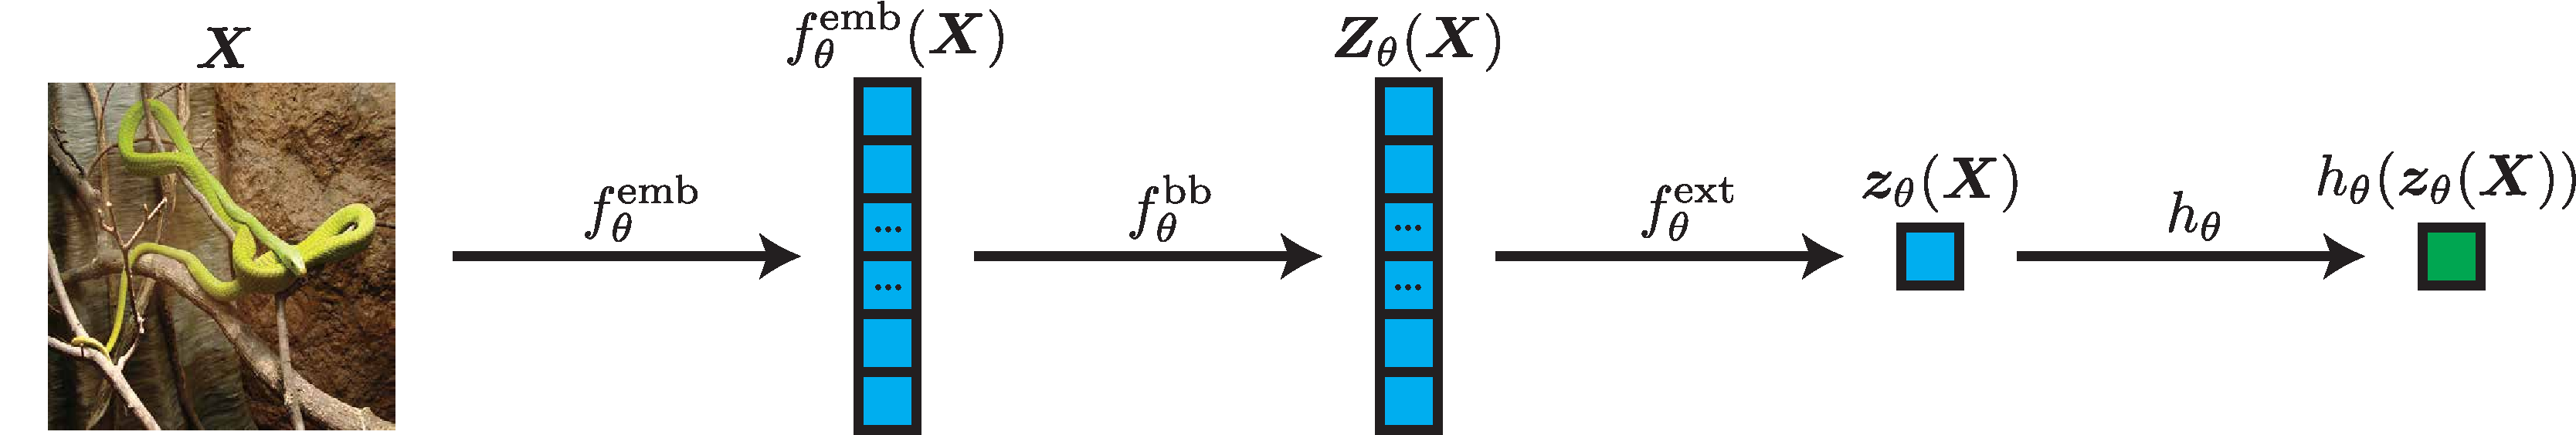
\includegraphics[width=\textwidth]{\toplevelprefix/chapters/chapter7/figs/encoder_pipeline.pdf}
    \caption{\small\textbf{A diagram of the encoder pipeline.} Data \(\vX \in \cD\) is fed through the embedding \(f_{\theta}^{\emb}\) to get a sequence in \((\R^{d})^{*}\). The embedding is fed through a backbone \(f_{\theta}^{\mathrm{bb}}\) to get features \(\vZ_{\theta}(\vX)\) for each token. We can extract an aggregate feature \(\vz_{\theta}(\vX)\) using the extraction map \(f_{\theta}^{\mathrm{ext}}\). Finally, to use the aggregate feature in downstream tasks, we can use the task-specific head \(h_{\theta}\).}
    \label{fig:overall_encoder_pipeline}
\end{figure}

\begin{figure}
    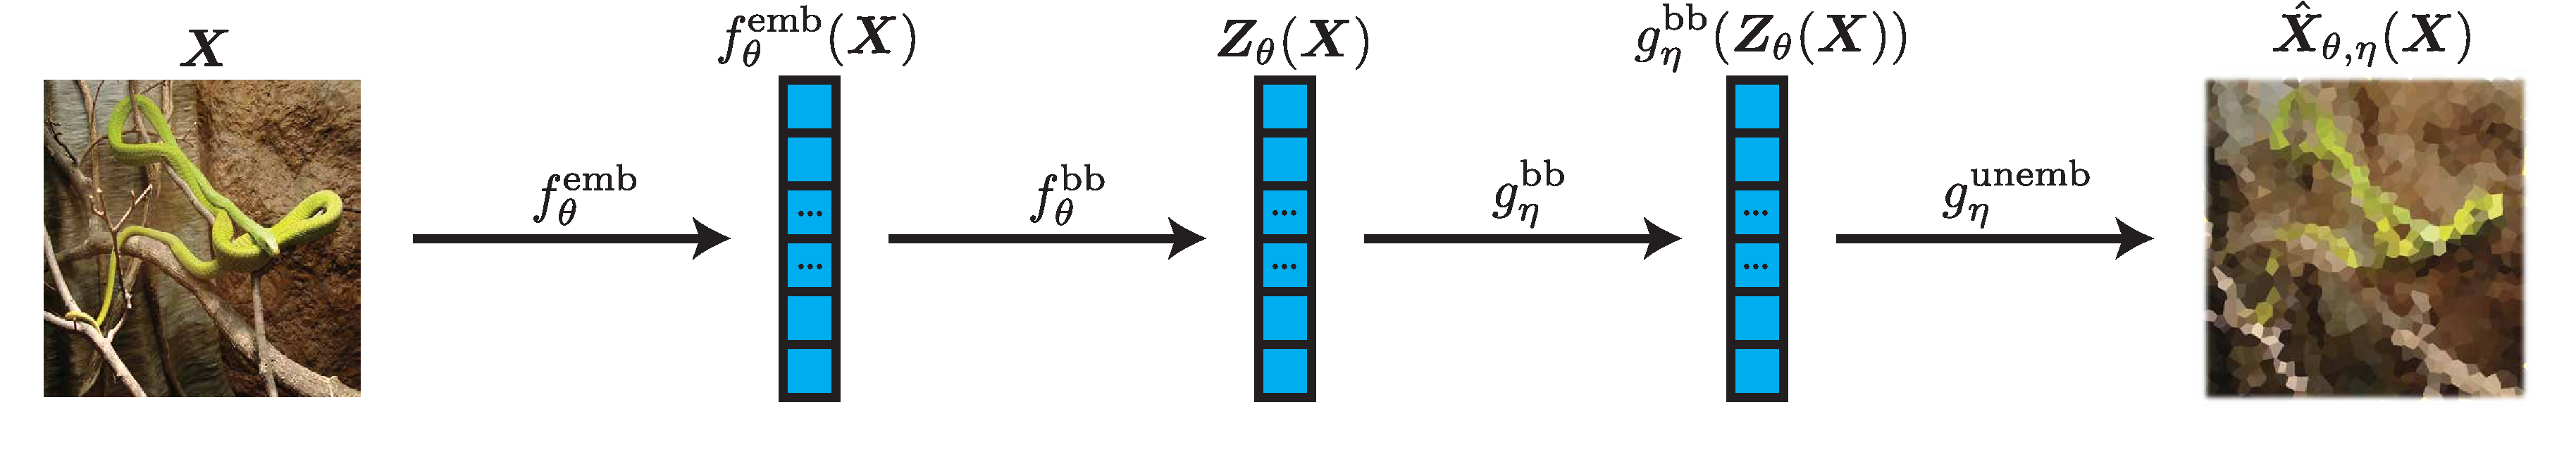
\includegraphics[width=\textwidth]{\toplevelprefix/chapters/chapter7/figs/autoencoder_pipeline.pdf}
    \caption{\small\textbf{A diagram of the autoencoder pipeline.} Data \(\vX \in \cD\) is fed through the embedding \(f_{\theta}^{\emb}\) to get a sequence in \((\R^{d})^{*}\). The embedding is fed through an encoder backbone \(f_{\theta}^{\mathrm{bb}}\) to get features \(\vZ_{\theta}(\vX)\) for each token. To decode \(\vZ_{\theta}(\vX)\), we pass it through a decoder backbone \(g_{\eta}^{\mathrm{bb}}\). To map the decoder backbone output back to data space \(\cD\), we use an \textit{unembedding} layer \(g_{\eta}^{\mathrm{unemb}}\), overall obtaining a reconstruction \(\hat{\vX}_{\theta, \eta}(\vX)\) (here stylized to be a pixelated reconstruction of the input).}
    \label{fig:overall_autoencoder_pipeline}
\end{figure}

Let us define the set of possible data as \(\cD\) (eventually this will be the set of images \(\cI\), for example, or the set of text \(\cT\)), and the set of finite sequences of tokens in \(\R^{d}\) (i.e., the set of matrices with \(d\) rows) as \((\R^{d})^{*} \doteq \bigcup_{T = 1}^{\infty}\R^{d \times T}\). In order to discuss the wealth of applications we introduce in this chapter, we first recall that in the rest of the book, we discuss two different types of model architectures.
\begin{itemize}
    \item An \textit{encoder} architecture, parameterized by \(\theta\), which is composed of several components:
    \begin{itemize}
        \item An \textit{embedding} \(f_{\theta}^{\emb} \colon \cD \to (\R^{d})^{*}\), which converts the input data \(\cD\) into a series of \textit{tokens} which are mapped into, or \textit{embedded} in, \(d\)-dimensional space. \textit{In the rest of the chapter, we will often identify tokens and embeddings with each other.}
        \item An \textit{encoder backbone} \(f_{\theta}^{\backbone} \colon (\R^{d})^{*} \to (\R^{d})^{*}\), which processes the series of embeddings using a sequence-to-sequence operation. This backbone is implemented by the network architectures discussed in the previous chapters, but we will give a more formal description as we go along.
        \item An \textit{aggregate feature extractor} \(f_{\theta}^{\ext} \colon (\R^{d})^{*} \to \R^{d}\), which extracts an aggregate representation of the whole sequence. This is used to define a single feature for the entire data sample.
        \item A \textit{task-specific head} \(h_{\theta} \colon \R^{d} \to \R^{m}\), which extracts an \(m\)-dimensional output for prediction.
    \end{itemize}
    We also define \(f_{\theta} \doteq f_{\theta}^{\backbone} \circ f_{\theta}^{\emb} \colon \cD \to (\R^{d})^{*}\). Given an input \(\vX\), we write \(\vZ_{\theta}(\vX) \doteq f_{\theta}(\vX)\) and \(\vz_{\theta}(\vX) \doteq f_{\theta}^{\ext}(\vZ_{\theta}(\vX))\). The overall pipeline is depicted in \Cref{fig:overall_encoder_pipeline}.
    \item An \textit{autoencoder} architecture, which is composed of several components:
    \begin{itemize}
        \item An \textit{embedding} \(f_{\theta}^{\emb} \colon \cD \to (\R^{d})^{*}\), which converts the input data \(\cD\) into a series of \textit{tokens} which are embedded in \(d\)-dimensional space.
        \item An \textit{encoder backbone} \(f_{\theta}^{\backbone} \colon (\R^{d})^{*} \to (\R^{d})^{*}\), which processes the series of embeddings using a sequence-to-sequence operation.
        \item A \textit{decoder backbone} \(g_{\eta}^{\backbone} \colon (\R^{d})^{*} \to (\R^{d})^{*}\), which conceptually undoes the operation of the encoder backbone.
        \item An \textit{unembedding} \(g_{\eta}^{\unemb} \colon (\R^{d})^{*} \to \cD\), which acts as an inverse of the embedding.
    \end{itemize}
    We also define \(f_{\theta} \doteq f_{\theta}^{\backbone} \circ f_{\theta}^{\emb} \colon \cD \to (\R^{d})^{*}\) and \(g_{\eta} \doteq g_{\eta}^{\unemb} \circ g_{\eta}^{\backbone} \colon (\R^{d})^{*} \to \cD\). Given an input \(\vX\), we write \(\vZ_{\theta}(\vX) \doteq f_{\theta}(\vX)\) and \(\hat{\vX}_{\theta, \eta}(\vX) \doteq g_{\eta}(\vZ_{\theta}(\vX))\). The overall pipeline is depicted in \Cref{fig:overall_autoencoder_pipeline}.
\end{itemize}

We will repeatedly use this notation many times in this chapter, so please feel free to refer back to it if something doesn't make sense. This decomposition of our networks also closely mirrors most code implementations, and you can start your coding projects by defining these networks.

In this chapter, we will discuss applications of the book's principles to contrastive learning in \Cref{sec:contrastive_learning}. This will serve as both an introduction to image data, data augmentation techniques, and the common architecture known as the transformer, \textit{as well as} a first demonstration of the drastic kinds of simplifications we can make using the demonstrated principles. We will continue with modifications to the \textit{network architecture} in \Cref{sec:image_classification,sec:clm_text}, which demonstrate the capabilities of simplified architectures for \textit{encoding} within the image and text domains. We then demonstrate simplified architectures for \textit{autoencoding} in \Cref{sec:image_completion}. %


\section{Simplified Contrastive Learning}\label{sec:contrastive_learning}

Learning high-quality and faithful representations of data is a fundamental problem in deep learning, known as \textit{self-supervised learning}. There have been many approaches proposed for this task, many of which do not evidently use the techniques and principles outlined in this manuscript. One such approach is called \textit{contrastive learning}, so named because the learning objective is (roughly speaking) about ensuring that features of ``similar'' data are similar, and features of ``dissimilar'' data are far apart. Contrastive learning solutions are often highly-engineered, empirically designed approaches. In this section, we will describe one such approach named DINO \citep{caron2021emerging}, and use the principles described in the previous chapters to drastically simplify their design decisions while improving the learned representations.

\subsection{Data}\label{sub:contrastive_learning_data}

The data that we will use to explore and simplify the DINO methodology are all 2-dimensional image data. For \textit{training}, we will use the ImageNet-1K and ImageNet-21K datasets. Each sample in the dataset is an RGB image, of varying resolution, and a label indicating the object or scene that the image contains (i.e., the \textit{class} of the image). The ImageNet-1K dataset contains 1.28M training images and 50K validation images partitioned into 1K classes. The ImageNet-21K dataset contains 14.2M training images and 21.8K classes, but the classes are not disjoint (i.e., some classes are subsets of others). Since we are doing self-supervised learning, the labels will not be used during training, only during evaluation. For \textit{evaluation}, we will use a litany of datasets. Of these, the most common is CIFAR-10. CIFAR-10 is a dataset of 60K RGB 32 \(\times\) 32 natural images partitioned into 10 classes, with a pre-established training set of 50K samples and a validation set of 10K samples. The purpose of using CIFAR-10 is to ensure that models which train on one distribution of images (ImageNet) can generalize to another distribution of images (CIFAR-10). We also refer to other similar datasets, such as CIFAR-100 (disjoint from CIFAR-10), Oxford Flowers, and Oxford Pets. Exemplars of ImageNet-1K and CIFAR-10 data are shown in \Cref{fig:in1k_cifar10_examples}. In order to increase the robustness of our model, we often apply \textit{small data augmentations} to each image during processing, such as flips, added small random noise, or random large crops; we do not include this in our notation, as each augmentation of a natural image is itself (very close to) a natural image in our dataset.

\begin{figure}
    \centering
    
    \hfill 
    \begin{subfigure}{0.3\textwidth}
        \centering 
        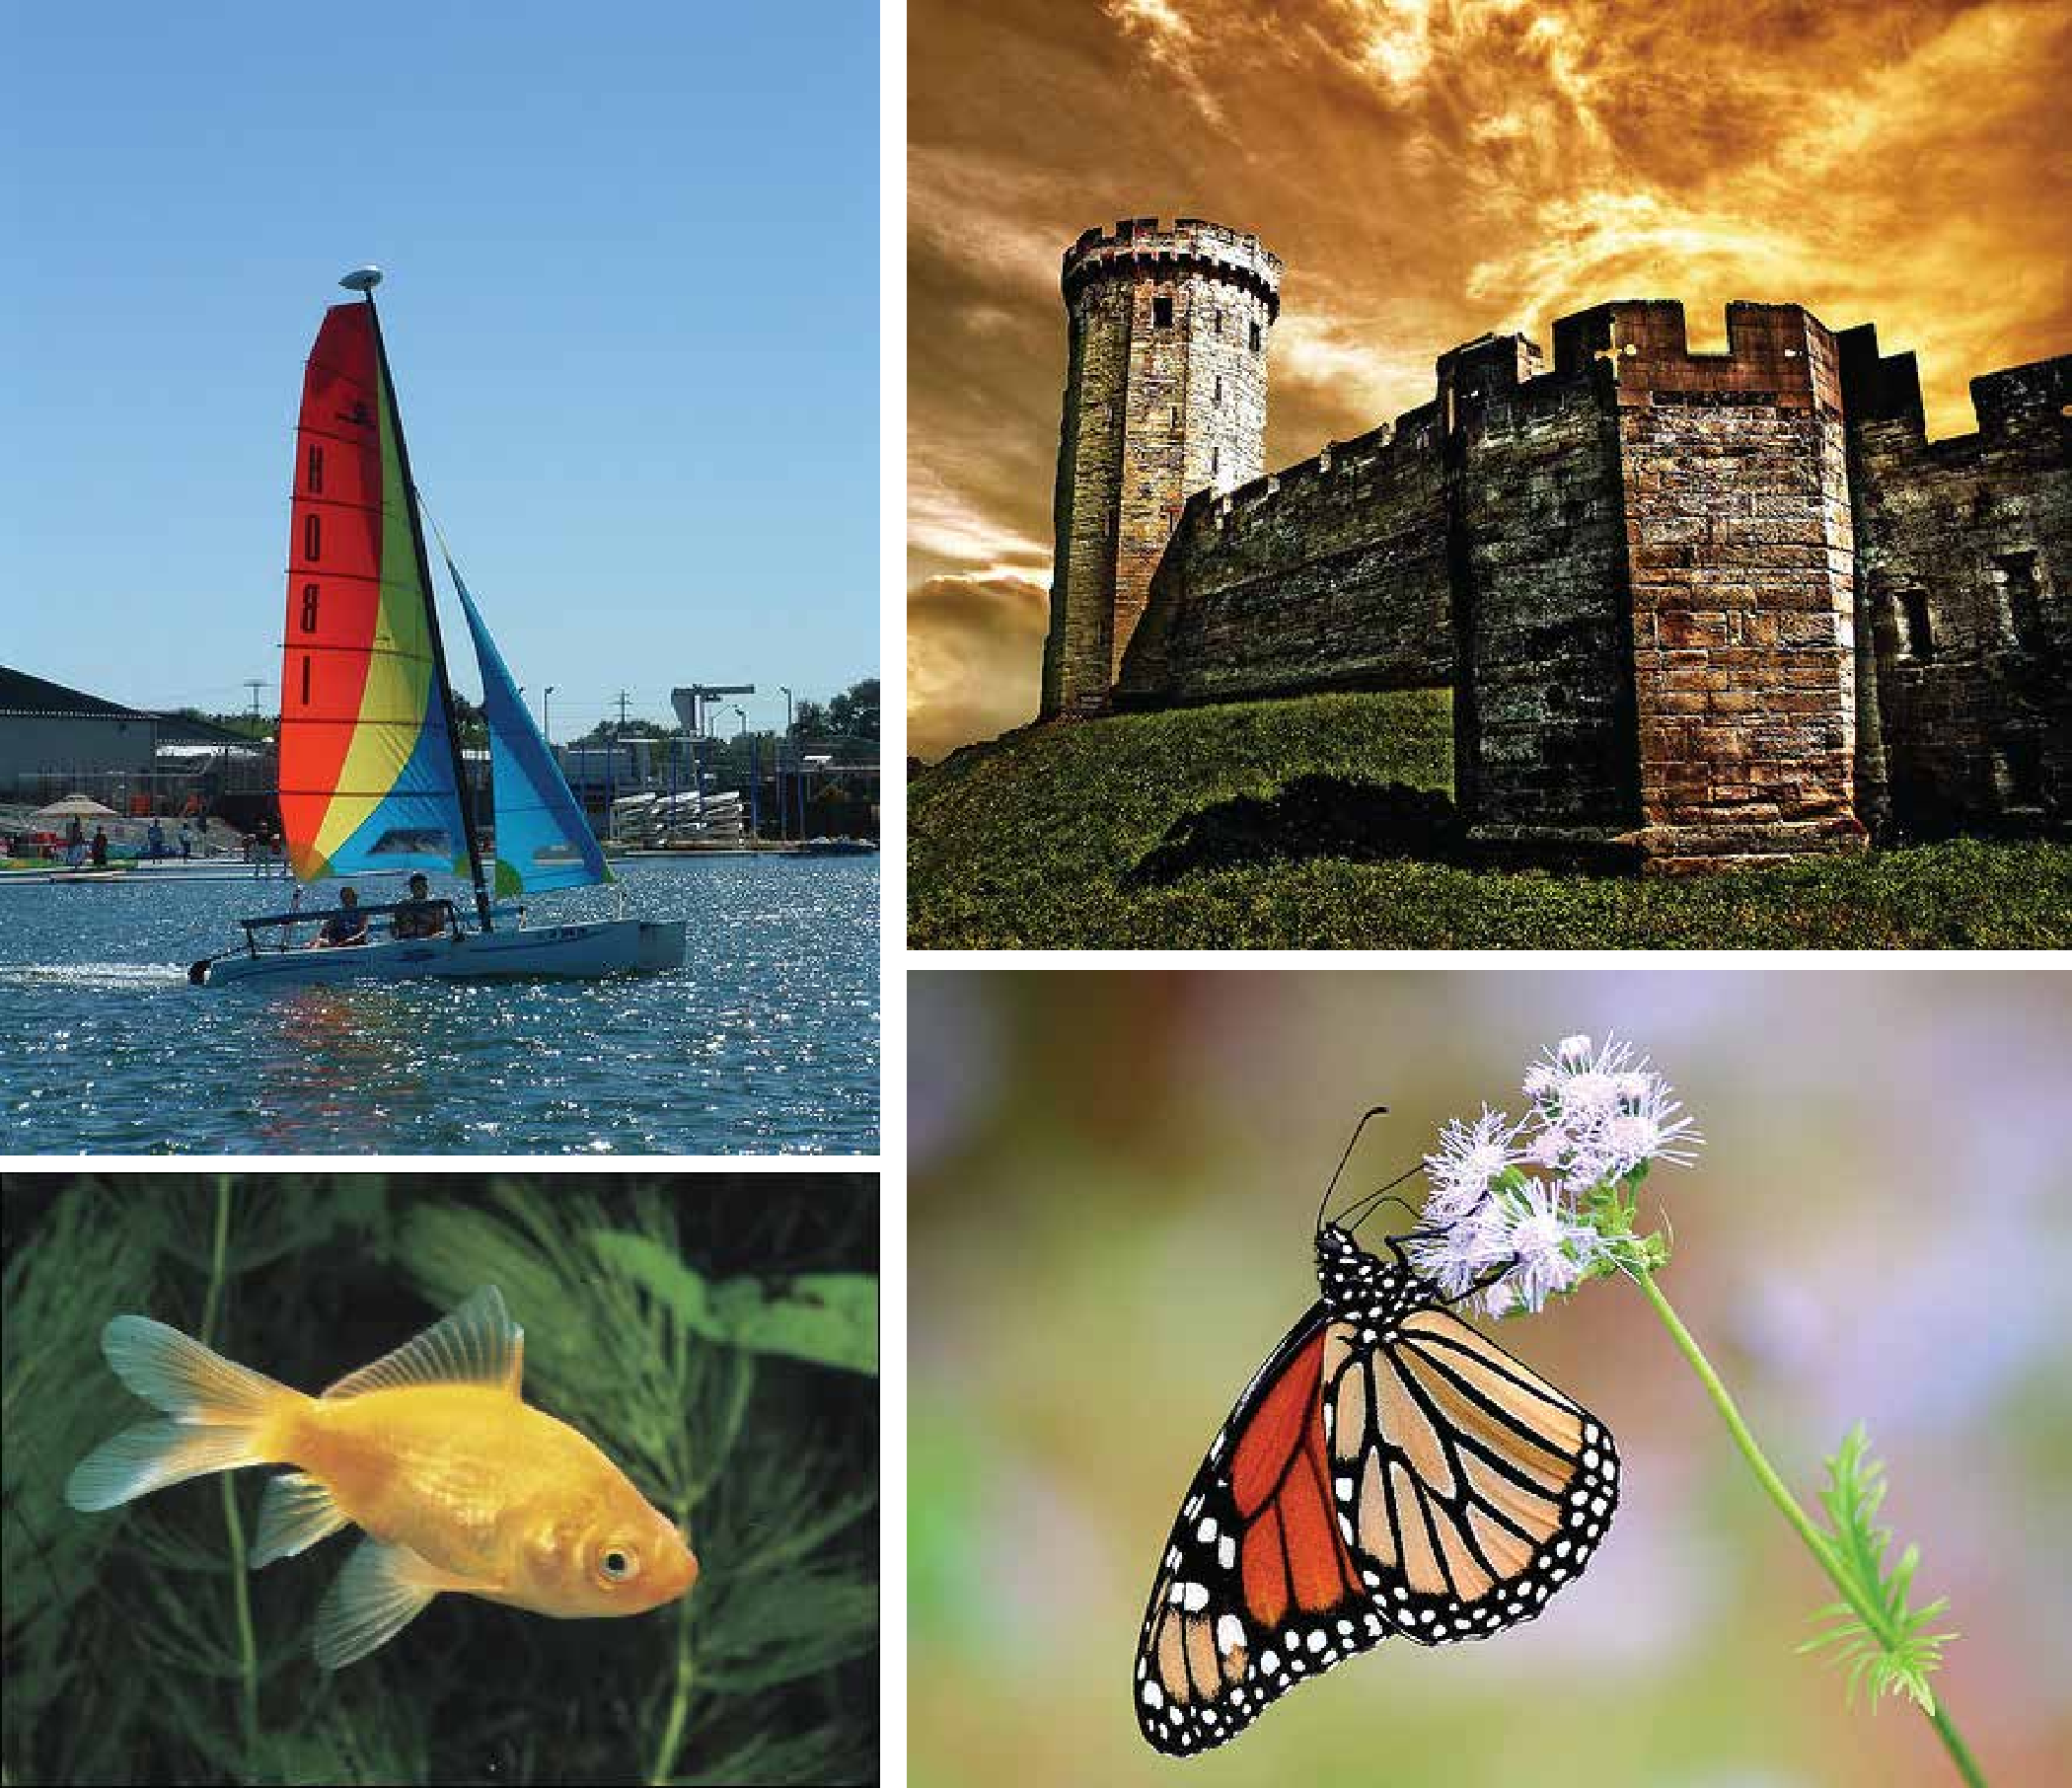
\includegraphics[width=\textwidth]{\toplevelprefix/chapters/chapter7/figs/imagenet.pdf}
        \caption{\small ImageNet-1K samples.}
    \end{subfigure}
    \hfill 
    \begin{subfigure}{0.26\textwidth}
        \centering 
        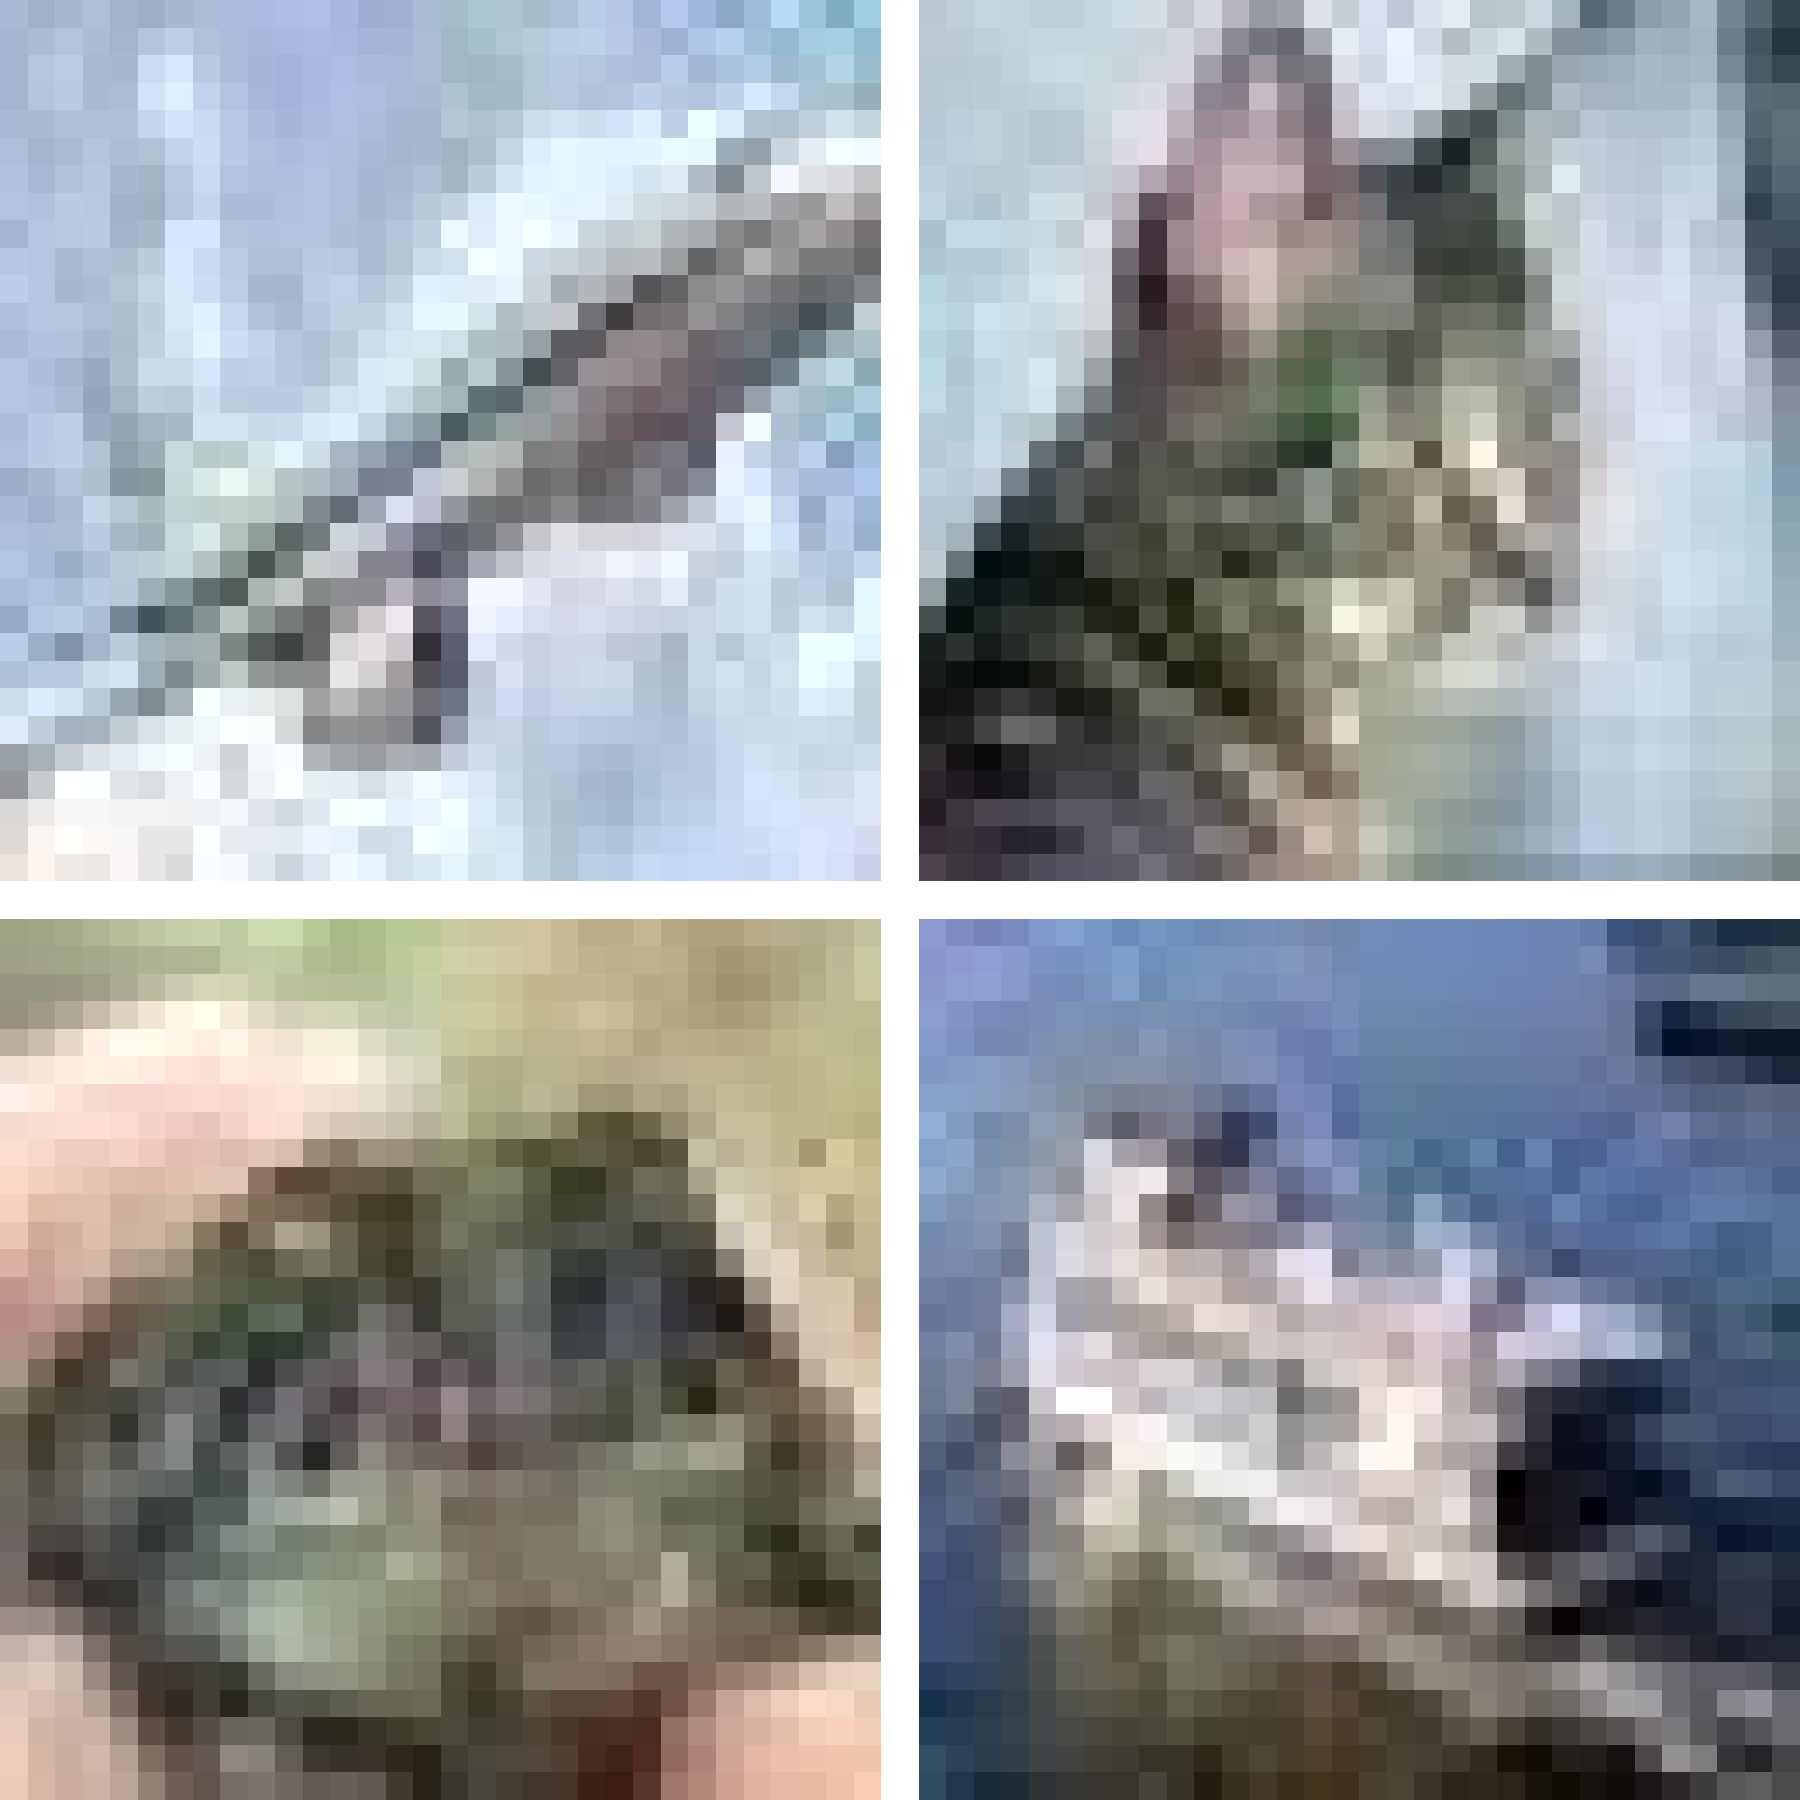
\includegraphics[width=\textwidth]{\toplevelprefix/chapters/chapter7/figs/cifar10.pdf}
        \caption{\small CIFAR10 samples.}
    \end{subfigure}
    \hfill 
    \phantom{}

    \caption{\small\textbf{Images from ImageNet-1K \textit{(left)} and CIFAR-10 \textit{(right)}.} Notice that the CIFAR-10 images are much lower resolution, generally speaking, reducing the complexity of learning that distribution.}
    \label{fig:in1k_cifar10_examples}
\end{figure}

On a slightly more formal level, our data \(\vX\) will be images; we let \(\cI\) be the set of all images. Since an image is a rectangular array of pixels, and each pixel has a color given by RGB, CMYK, or another color format, we say that an image is an element of \(\R^{c \times h \times w}\) --- here \(c\) is the number of channels (i.e., \(3\) for RGB and \(4\) for CMYK), \(h\) is the image height, and \(w\) is the image width. Consequently, the set of all images \(\cI \doteq \bigcup_{c, h, w = 1}^{\infty}\R^{c \times h \times w}\) is the set of all possible such data. Again, we will use this notation repeatedly.


\subsection{Task and Objective Function} \label{sub:contrastive_learning_objective}

Our task is to learn a good representation of the data. Contrastive learning, by and large, does this by defining what properties of the input image we wish the features to reflect, constructing images which share these properties but vary others, and setting up a loss which promotes that the features of images with shared properties are close and images with different properties are different. The naturally optimal solution to this learning problem is that the learned features preserve the desired properties of the input. However, there are many practical and empirical complications that arise in the course of training contrastive models.

In the case of DINO, the authors propose to use a methodology which produces a single feature vector for the whole image and desires the feature vector to contain ``global'' (i.e., image-level) information. Accordingly, the loss will promote that images with similar global information have similar features and images with different global information have different features.

This seems intuitive, but as previously mentioned, there are several empirical considerations, even while setting up the loss. First and foremost, how should we promote similarities and differences? The answer from DINO \citep{caron2021emerging} is\footnote{In the author's view, inexplicably...} to convert the output features into ``logits'' corresponding to some probability distribution and take their cross-entropy. More specifically, let \(\Delta_{m} \doteq \{\vx \in \R^{m} \colon x_{i} \geq 0\ \forall i \in [m], \sum_{i = 1}^{m}x_{i} = 1\}\) be the space of probability vectors in \(\R^{m}\) and define the function \(d_{\CE} \colon \R^{m} \times \R^{m} \to \R\) by
 \begin{equation}\label{eq:cross_entropy_difference}
    d_{\CE}(\vp, \vq) \doteq \CE(\vp, \vq), \quad \forall \vp, \vq \in \Delta_{m}
 \end{equation}
 where \(\CE \colon \Delta_{m} \times \Delta_{m} \to \R\) is the cross-entropy, defined as 
 \begin{equation}\label{eq:expts_def_ce}
    \CE(\vp, \vq) \doteq -\sum_{i = 1}^{m}p_{i}\log q_{i}, \quad \forall \vp = (p_{1}, \dots, p_{m}), \vq = (q_{1}, \dots, q_{m}) \in \Delta_{m}.
 \end{equation}
 Before we continue our discussion, let us build some intuition about this distance function. We have, in particular,
 \begin{align}
    \CE(\vp, \vq)
    &= -\sum_{i = 1}^{m}p_{i}\log q_{i} = \sum_{i = 1}^{m}p_{i}\log(p_{i}/q_{i})
     - \sum_{i = 1}^{m}p_{i}\log p_{i} = \KL(\vp\mmid \vq) + H(\vp)
 \end{align}
 where \(\KL \colon \Delta_{m} \times \Delta_{m} \to \R\) is the KL divergence, defined as 
 \begin{equation}
    \KL(\vp\mmid \vq) \doteq \sum_{i = 1}^{m}p_{i}\log(p_{i}/q_{i}),
 \end{equation}
 and \(H \colon \Delta_{m} \to \R\) is the entropy of a random variable. Note
 that \(\KL(\vp\mmid \vq)\) is minimized if and only if \(\vp = \vq\). So minimizing \(d_{\CE}\) does two things: it makes \(\vp = \vq\), and it makes \(\vp\) and \(\vq\) have minimal entropy (i.e., vectors with \(1\) in one component and \(0\) elsewhere --- these are called \textit{one-hot vectors}). Overall, the goal of this objective is not \textit{just} to match \(\vp\) and \(\vq\) but also to shape them in a certain way to make them low-entropy. Keep this in mind when we discuss the formulation.

The next question is, how should we obtain samples with similar global information? The answer from DINO (as well as nearly all contrastive learning) is \textit{data augmentation} --- from each sample, make several correlated samples which share the desired properties. In the DINO case, we use different crops or \textit{views} of the input image. Recall that we model an image as an element of the set \(\cI\). In this notation, a view is a function \(v \colon \cI \to \cI\). In the DINO case, the view is a \textit{random resized crop}: it takes a randomly chosen rectangular crop of the image (which has a fixed percentage \(p_{v} \in [0, 1]\) of the total area of the image), resizes it proportionally so that the \textit{shorter edge} is \(S_{\rsz}\) pixels long, then resizes it to a fixed shape \((C, S_{v}, S_{v})\) where \(S_{v} \geq 1\) is the size of the view and \(C\) is the number of channels in the original image. 

\begin{figure}
    \centering 
    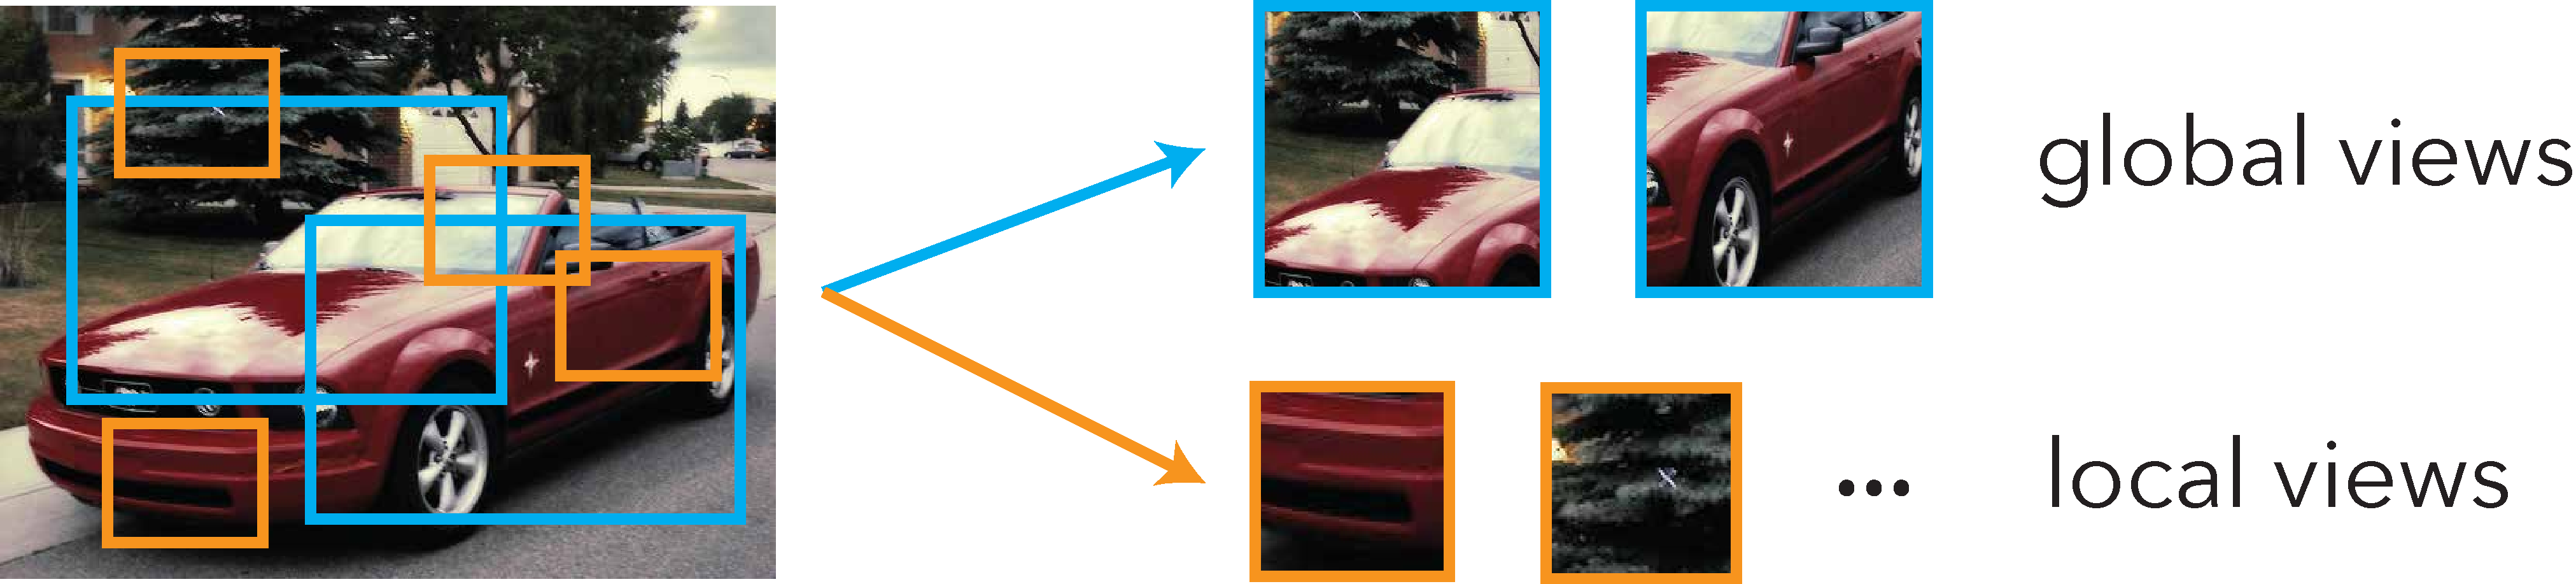
\includegraphics[width=0.7\textwidth]{\toplevelprefix/chapters/chapter7/figs/global_local_views.pdf}
    \caption{\textbf{Local and global views in DINO.} Local views and global views take a rectangular crop of the input image and resize it to a square shape, which is then input into the network for processing.}
    \label{fig:dino_local_global_views}
\end{figure}

There are two types of views we want to use, depicted in \Cref{fig:dino_local_global_views}: 
\begin{itemize}
    \item \textit{global views}, which are random resized crops with area percentage parameter \(p_{\glo} \in [0, 1]\) and output shape \((C, S_{\glo}, S_{\glo})\);
    \item \textit{local views}, which are random resized crops with area percentage parameter \(p_{\loc} \in [0, 1]\) and output shape \((C, S_{\loc}, S_{\loc})\). Here \(p_{\loc} < p_{\glo}\) and \(S_{\loc} < S_{\glo}\).
\end{itemize}

DINO desires that the aggregate features \(\vz_{\theta}(\vX_{v}) \doteq (f_{\theta}^{\ext} \circ f_{\theta})(\vX_{v})\) of all views \(\vX_{v} \doteq v(\vX)\) of an input image \(\vX\) be consistent with each other. DINO does this by using a \textit{``DINO head''}\footnote{Note that \(h_{\vW, \vmu}\) is the task-specific head, which in \Cref{sec:experiment_setup} is parameterized only by \(\theta\) as opposed to any specific parameters, but since we use two invocations of \(h\) with different values of the second parameter, we keep the specified notation.} \(h_{\vW, \vmu}\), parameterized by a matrix \(\vW \in \R^{s \times d}\) and a vector \(\vmu \in \R^{s}\), to extract a probability vector \(\vp_{\theta, \vW, \vmu}(\vX_{v}) \doteq h_{\vW, \vmu}(\vz_{\theta}(\vX_{v}))\) from the aggregate feature \(\vz_{\theta}(\vX_{v})\), using the following simple recipe:
\begin{equation}
    h_{\vW, \vmu}(\vz) \doteq \softmax([\vW\vz - \vmu]/\tau), \qquad \forall \vz \in \R^{d},
\end{equation}
where the \(\softmax \colon \R^{s} \to \Delta_{s}\) function is defined by 
\begin{equation}
    \softmax\rp{\mat{x_{1} \\ \vdots \\ x_{s}}} \doteq \frac{1}{\sum_{i = 1}^{s}e^{x_{i}}}\mat{e^{x_{1}} \\ \vdots \\ e^{x_{s}}}
\end{equation}
and \(\tau > 0\) is a ``temperature'' parameter which controls the entropy of the softmax's output.

In particular, DINO minimizes the difference between the probability vector \(\vp_{\theta, \vW, \vmu}(\vX_{g}) \doteq h_{\vW, \vmu}(\vz_{\theta}(\vX_{g}))\) for each global view \(\vX_{g} \doteq v_{g}(\vX)\) and the probability vector \(\vp_{\theta, \vW}(\vX_{c}) \doteq h_{\vW, \vzero_{m}}(\vz_{\theta}(\vX_{c}))\) for each view \(\vX_{c} \doteq v_{c}(\vX)\). Here, \(v_{c}\) can \textit{either} be a local view or a global view. We will discuss the implementation of \(f_{\theta}\) and \(f_{\theta}^{\ext}\) shortly in \Cref{sub:contrastive_learning_architecture}. Overall, DINO solves the problem
 \begin{equation}\label{eq:dino_loss}
     \min_{\theta, \vW, \vmu}\cL_{\dino}(\theta, \vW, \vmu) \qquad \text{where} \qquad \cL_{\dino}(\theta, \vW, \vmu) \doteq \Ex[d_{\CE}(\vp_{\theta, \vW, \vmu}(\vX_{g}), \vp_{\theta, \vW}(\vX_{c}))],
\end{equation}
where the expectation is over data \(\vX\), global views \(v_{g}\), and other views \(v_{c}\).

In this specific case, however, if you try to implement \eqref{eq:dino_loss} and optimize it on a real network, it is very likely that you will run into a problem: after running a few iterations of the learning algorithm, the feature mapping \(f_{\theta}^{\ext} \circ f_{\theta}\) will \textit{become the constant function}! This certainly optimizes the above loss since it minimizes the distance between features of different views of the same image. But we obviously do not want to learn this solution. 

Actually avoiding collapse is a very common consideration in contrastive learning. So how do we do it in this case? The solution from DINO, again, is empirically designed, and carefully tunes the optimization of the parameter \(\vmu\) (which is updated using all samples in the batch) and a ``temperature'' hyperparameter \(\tau\) which is part of the implementation of \(h_{\vW, \vmu}\) and discussed in \Cref{sub:contrastive_learning_architecture}. Given a certain special set of hyperparameters that work well, this is indeed enough to ensure non-collapse of the representation. However, outside of this special configuration, training models to converge is difficult, and the training is highly unstable. 

To amend this state of affairs, let us discuss simplifications to the formulation. First, instead of computing a probability vector using a learned transformation \(h_{\vW, \vmu}\) of the aggregate features \(\vz_{\theta}\), we can \textit{directly use the aggregate representation}, ignoring the task-specific head (or equivalently, setting it to the identity mapping). But now we need a way to compare the vectors directly. Using our hypothesis from \Cref{ch:representation} that good representations should have Euclidean (subspace) geometry, a much more natural measure of difference is the \textit{squared \(\ell^{2}\) distance} \(d_{\ell^{2}} \colon \R^{d} \times \R^{d} \to \R\), defined as 
\begin{equation}\label{eq:cosine_similarity}
    d_{\ell^{2}}(\vx, \vy) \doteq \frac{1}{2}\norm{\vx - \vy}_{2}^{2}, \qquad  \forall \vx, \vy \in \R^{d}.
\end{equation}
This distance-based score is even more efficient to compute than the cross-entropy score. Thus, \(d_{\ell^{2}}\) takes the place of \(d_{\CE}\) in our simplification. 

Before, collapse was avoided by using tricks to update \(\vmu\) and \(\tau\). In our simplification, if we compare the features within the representation space instead of converting them to probabilities, we do not have either of these parameters and so must consider a different way to avoid collapse. To do this, we return to the fundamentals. The basic idea of avoiding collapse is that in order to make sure that all samples do not return the same exact same features, we need different samples to have different features. In other words, we would like the \textit{covariance} of the features to be \textit{large} in some sense. But from \Cref{ch:compression,ch:representation}, we already have a quantity which measures the size of the covariance matrix. Namely, we use the straightforward (population-level) \textit{Gaussian coding rate} \(R\) to ensure that the features of global views of different images, which have different global information, are well-separated and not collapsed (hence expanded). The overall modified loss \(\cL_{\simdino}\) becomes:
\begin{equation}\label{eq:simdino_loss}
    \cL_{\simdino}(\theta) \doteq \Ex[d_{\ell^{2}}(\vz_{\theta}(\vX_{g}),
    \vz_{\theta}(\vX_{c}))] - \frac{\gamma}{2}\log\det\rp{\vI + \frac{d}{\eps^{2}}\Cov(\vz_{\theta}(\vX_{g}))},
\end{equation}
where \(\eps > 0\) is fixed and the appropriate expectations are, as before, taken over data \(\vX\), global view \(v_{g}\), and other (local or global) view \(v_{c}\). The loss in \eqref{eq:simdino_loss} is the loss used for the simplified DINO (``SimDINO''). As we will see, when properly implemented, it works at least as well as the original DINO.

\subsection{Architecture: Vision Transformer}\label{sub:contrastive_learning_architecture}

For the architecture, we use a standard vision transformer. Here is how such an architecture works formally in the context of image data. Recall from \Cref{sec:experiment_setup} that there are four components to an encoder architecture, namely an embedding, a backbone, a feature extractor, and a task-specific head. We discuss these four parts presently.

\begin{figure}
    \centering 
    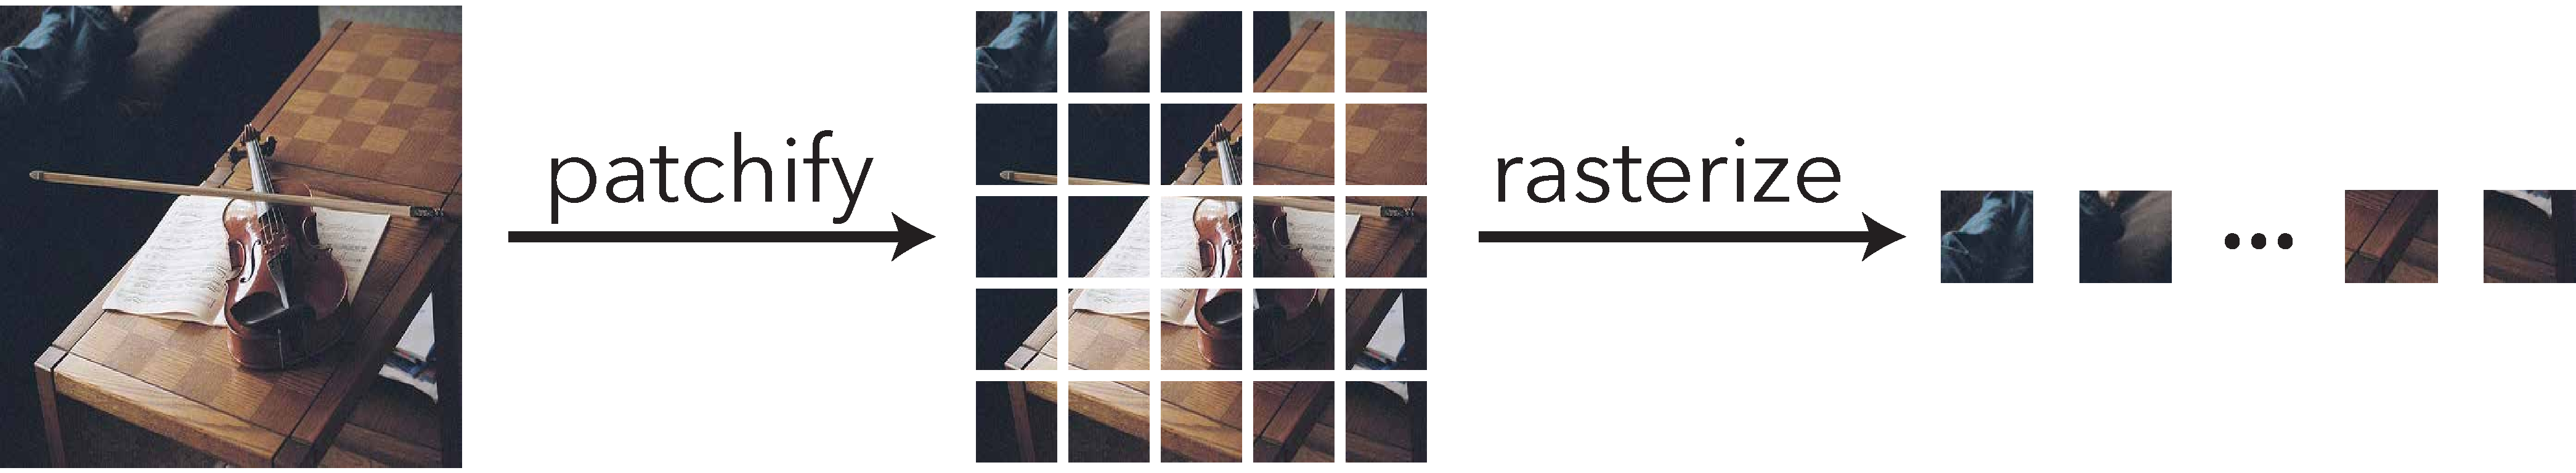
\includegraphics[width=0.8\textwidth]{\toplevelprefix/chapters/chapter7/figs/patchify.pdf}
    \caption{\small\textbf{An example of an image turned into \(5 \times 5\) square patches, which are placed in raster order.} Each patch is of the same size, and the grid of patches is of shape \((N_{H}, N_{W}) = (5, 5)\). The grid of patches is then unrolled into a sequence of length \(5 \times 5 = 25\) in raster order.}
    \label{fig:patchify_rasterize}
\end{figure}

\begin{figure}
    \centering 
    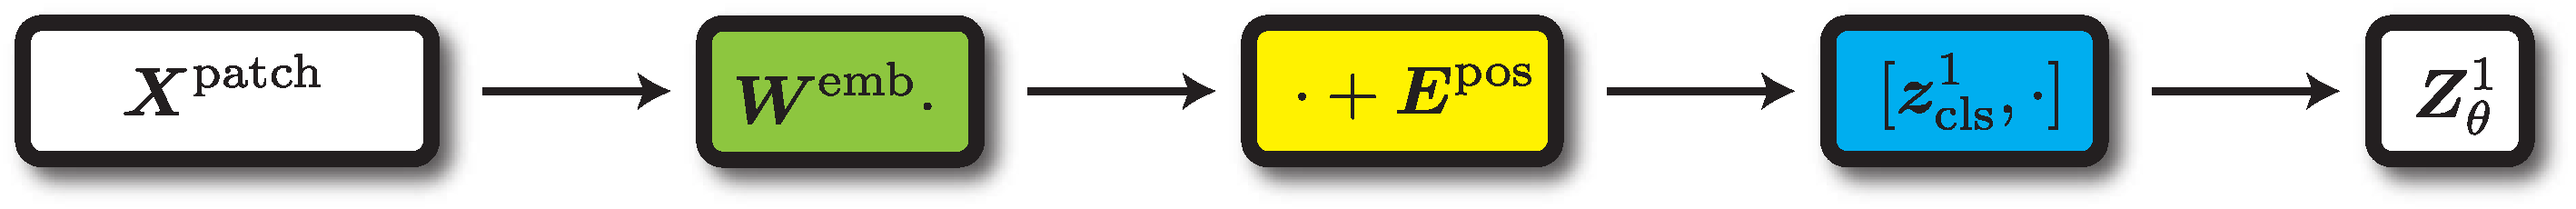
\includegraphics[width=\textwidth]{\toplevelprefix/chapters/chapter7/figs/transformer_embedding.pdf}
    \caption{\small\textbf{The transformer embedding pipeline.} Given a sequence of unrolled patches in raster order \(\vX^{\patch}\), each unrolled patch is linearly projected into the feature space, and equipped with an (additive) positional encoding and an additional token known as the class token. The output is the first-layer-input feature \(\vZ_{\theta}^{1}(\vX) = f_{\theta}^{\emb}(\vX)\).}
    \label{fig:transformer_embedding}
\end{figure}

\paragraph{Embedding.} Given image data \(\vX \in \cI\), we embed it as a sequence of tokens in \(\R^{d}\) using the map \(f_{\theta}^{\emb}\), as follows. The first two steps are depicted in \Cref{fig:patchify_rasterize}, and the latter two are depicted in \Cref{fig:transformer_embedding}.
\begin{enumerate}
    \item First, we turn the image data \(\vX\) into a sequence of patches of shape \((C, P_{H}, P_{W})\) where \(P_{H}\) and \(P_{W}\) are the patch dimensions. We assume that \(P_{H}\) and \(P_{W}\) evenly divide the height and width of \(\vX\), respectively (in the notation of \Cref{sub:contrastive_learning_objective} we assume that \(P_{H}\) and \(P_{W}\) evenly divide \(S_{\loc}\) and \(S_{\glo}\)). Let the resulting grid of patches have \(N_{H}\) rows and \(N_{W}\) columns.
    \item We unroll each patch into a vector of length \(D \doteq CP_{H}P_{W}\). There are \(N \doteq N_{H}N_{W}\) patch vectors, which we place in ``raster order'' (top left \(\to\) top right \(\to\) bottom left \(\to\) bottom right) into a matrix \(\vX^{\patch} \in \R^{D \times N}\), where \(\vX^{\patch} \doteq f^{\patch}(\vX)\). Notice that \(D\) depends only on the patch size and number of channels. Since the latter quantity is normally constant among samples in the same dataset, \(D\) is the same for all images in the dataset, while \(N\) is different for larger and smaller images.
    \item We then perform the following operation on \(\vX^{\patch} \in \R^{D \times N}\) to project it to \(\R^{d \times n}\) where \(n \doteq N + 1\):
    \begin{equation}
        \vX^{\patch} \mapsto [\vz_{\cls}^{1}, \vW^{\emb}\vX] + \vE^{\pos}.
    \end{equation}
    Here we have three trainable parameters \(\vW^{\emb}\), \(\vz_{\cls}^{1}\), and \(\vE^{\pos}\) whose purpose is as follows:
    \begin{itemize}
        \item \(\vW^{\emb} \in \R^{d \times D}\) is a matrix which projects each patch vector to a token feature.
        \item \(\vz_{\cls}^{1} \in \R^{d}\) is a so-called \textit{class token} or \textit{register token}. The class token heuristically holds global information of the whole data and is used for downstream tasks. In the framework of compressive deep networks from \Cref{ch:representation}, we expect that the class token is projected onto the same subspaces as the salient or semantically relevant tokens during the progression of the forward pass.
        \item \(\vE^{\pos} \in \R^{d \times N}\) is a so-called \textit{positional encoding} which distinguishes tokens of different patches from each other. That is, token features should have positional information, so that the overall map \(f^{\pre}\) is not invariant to permutations of the patches, and \(\vE^{\pos}\) inserts this positional information. 
        \begin{itemize}
            \item In this DINO case, where the transformer receives differently-sized images, we learn a positional encoding for the largest size received during training, and interpolate to get the positional encodings for smaller-sized inputs.
        \end{itemize}
    \end{itemize}
\end{enumerate}
Thus, in the end we have 
\begin{equation}\label{eq:definition_of_embedding_module}
    f_{\theta}^{\emb}(\vX) \doteq \mat{\vz_{\cls}^{1}, \vW^{\emb}f^{\patch}(\vX) + \vE^{\pos}}.
\end{equation}
All parameters \(\vz_{\cls}^{1}, \vW^{\emb}, \vE^{\pos}\) are contained in the parameter set \(\theta\).

\begin{figure}
    \centering 
    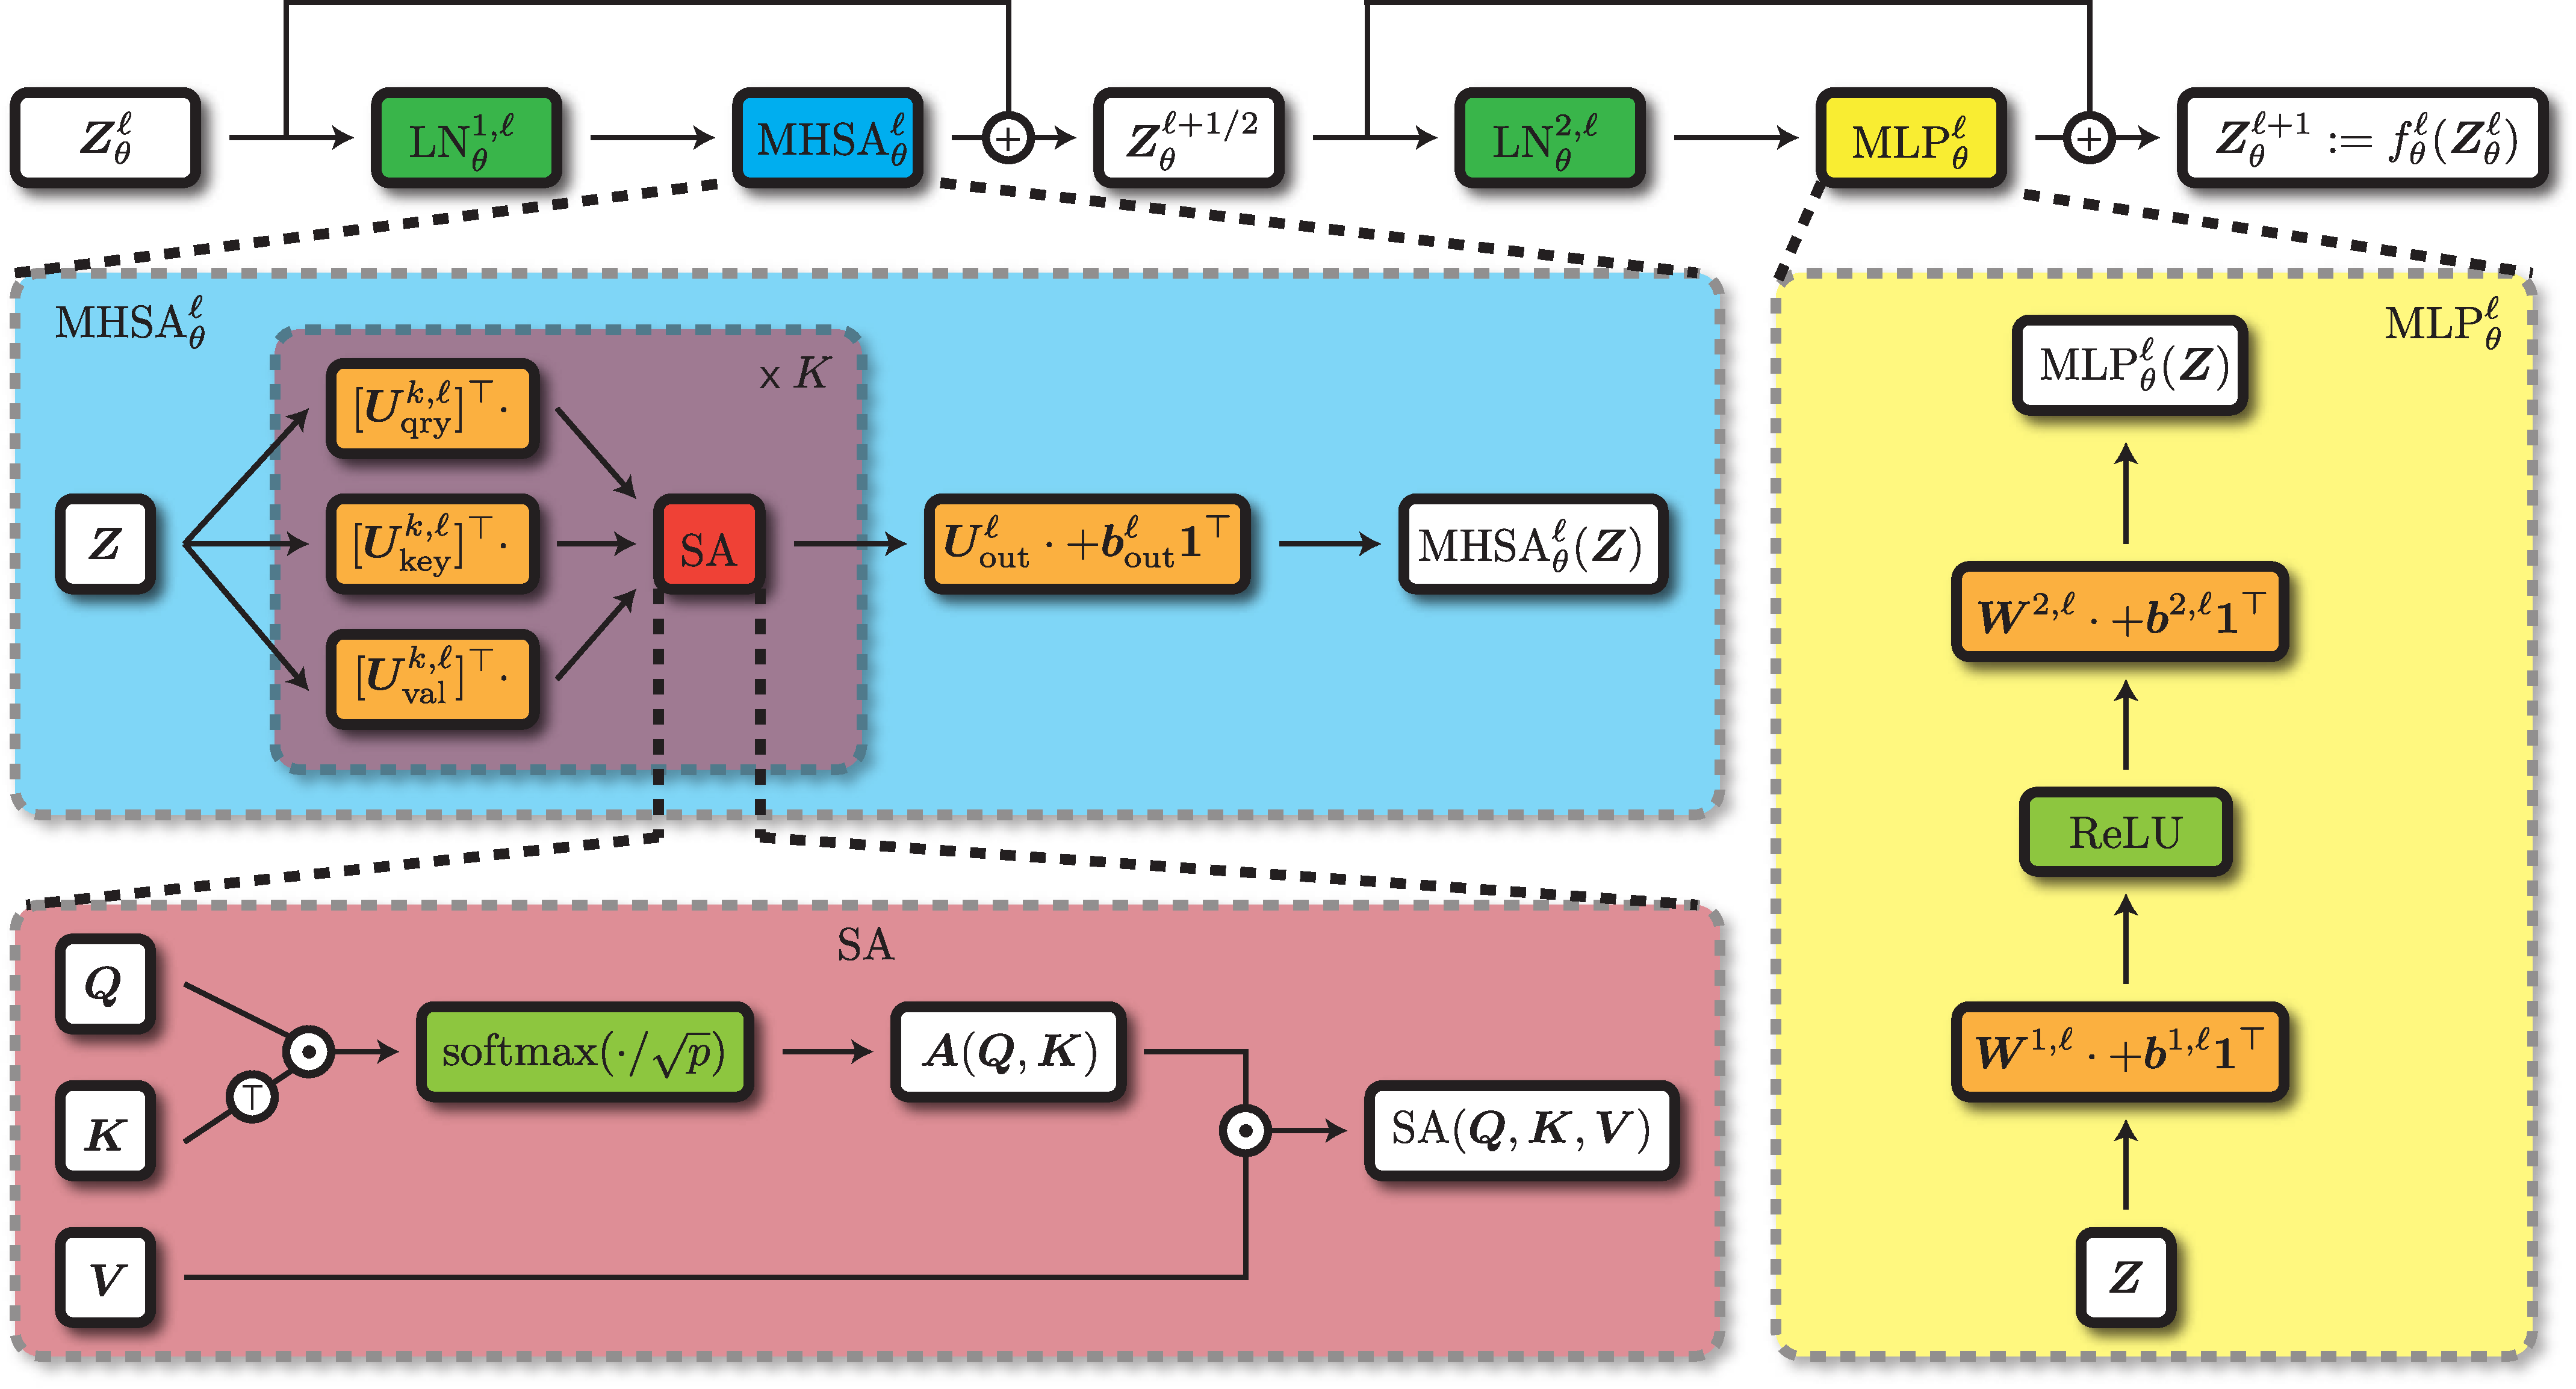
\includegraphics[width=\textwidth]{\toplevelprefix/chapters/chapter7/figs/transformer_backbone.pdf}
    \caption{\small\textbf{One layer \(f_{\theta}^{\ell}\) of the transformer backbone.} The input features go through layer-normalization, multi-head self-attention, and multi-layer perceptron blocks in sequence to form the output features of the layer.}
    \label{fig:transformer_backbone}
\end{figure}

\paragraph{Backbone.} Given a sequence of embeddings \(\vZ_{\theta}^{1}(\vX) \doteq f_{\theta}^{\emb}(\vX) \in (\R^{d})^{*}\), we process it using the backbone map \(f_{\theta}^{\backbone}\) as follows and as depicted in \Cref{fig:transformer_backbone}. The function \(f_{\theta}^{\backbone}\) is composed of \(L\) \textit{layers} \(f_{\theta}^{\ell}\), i.e.,
\begin{equation}
    f_{\theta}^{\backbone} = f_{\theta}^{L} \circ \cdots \circ f_{\theta}^{1}.
\end{equation}
 The layer \(f_{\theta}^{\ell}\) has the following implementation:
\begin{align}\label{eq:vit-res-block}
    \vZ_{\theta}^{\ell + 1/2}(\vX)
    &= \vZ_{\theta}^{\ell}(\vX) + \MHSA_{\theta}^{\ell}(\LN_{\theta}^{1, \ell}(\vZ_{\theta}^{\ell}(\vX))) \\ 
    \vZ_{\theta}^{\ell + 1}(\vX)
    &= \vZ_{\theta}^{\ell + 1/2}(\vX) + \MLP_{\theta}^{\ell}(\LN_{\theta}^{2, \ell}(\vZ_{\theta}^{\ell + 1/2}(\vX)))
\end{align}
and \(f_{\theta}^{\ell}\) is defined such that \(f_{\theta}^{\ell}(\vZ_{\theta}^{\ell}(\vX)) \doteq \vZ_{\theta}^{\ell + 1}(\vX)\). Here we have used some operators, such as \(\MHSA_{\theta}^{\ell}, \MLP_{\theta}^{\ell}\) and \(\LN_{\theta}^{i, \ell}\) that are defined as follows:
\begin{itemize}
    \item The \(\MHSA_{\theta}^{\ell}\) operator is multi-head-self-attention, the predecessor of the multi-head subspace self-attention (cf \Cref{ch:representation}). The formulation is as follows:
    \begin{align}
        \MHSA_{\theta}^{\ell}(\vZ) \label{eq:mhsa}
        &\doteq \vU_{\out}^{\ell}\mat{\SA([\vU_{\query}^{1, \ell}]^{\top}\vZ, [\vU_{\attnkey}^{1, \ell}]^{\top}\vZ, [\vU_{\val}^{1, \ell}]^{\top}\vZ) \\ \vdots \\ \SA([\vU_{\query}^{K, \ell}]^{\top}\vZ, [\vU_{\attnkey}^{K, \ell}]^{\top}\vZ, [\vU_{\val}^{K, \ell}]^{\top}\vZ)} + \vb_{\out}^{\ell}\vone_{n}^{\top}, \\
        \label{eq:self_attention}
        \text{where} \qquad \SA(\vQ, \vK, \vV)
        &\doteq \vV \underbrace{\softmax\rp{\frac{\vK^{\top}\vQ}{\sqrt{p}}}}_{\doteq \vA(\vQ, \vK)}
    \end{align}
    where \(p\) is a positive integer, \(\vU_{\query}^{k, \ell}, \vU_{\attnkey}^{k, \ell}, \vU_{\val}^{k, \ell} \in \R^{d \times p}\), \(\vU_{\out}^{\ell} \in \R^{d \times Kp}\), and \(\vb_{\out}^{\ell} \in \R^{d}\) are trainable parameters contained in the parameter set \(\theta\), and the \(\softmax\) is defined column-wise as 
    \begin{align}
        \softmax(\vM) 
        &\doteq \mat{\softmax(\vm_{1}) & \cdots & \softmax(\vm_{p})}, \\ 
        \forall \vM 
        &= \mat{\vm_{1}, \dots, \vm_{p}} \in \R^{n \times p}.
    \end{align}
    In practice, the dimensions are usually picked such that \(Kp = d\). The terms 
    \begin{equation}
        \label{eq:attention_map}
        \vA_{\theta}^{k, \ell}(\vZ) \doteq \vA([\vU_{\query}^{k, \ell}]^{\top}\vZ, [\vU_{\attnkey}^{k, \ell}]^{\top}\vZ), \qquad \SA_{\theta}^{k, \ell}(\vZ) \doteq \SA([\vU_{\query}^{k, \ell}]^{\top}\vZ, [\vU_{\attnkey}^{k, \ell}]^{\top}\vZ, [\vU_{\val}^{k, \ell}]^{\top}\vZ)
    \end{equation}
    are also known as the \textit{\(k\)th attention map} and \textit{\(k\)th attention head output} at layer \(\ell\), respectively. Furthermore, the operation \(\SA(\vQ, \vK, \vV)\) can be computed extremely efficiently using specialized software such as FlashAttention \citep{shah2025flashattention}.
    \item The \(\MLP_{\theta}^{\ell}\) is a two-layer perceptron, a regular nonlinearity used in deep networks, and has the form 
    \begin{equation}
        \MLP_{\theta}^{\ell}(\vZ) \doteq \vW_{\down}^{\ell}\ReLU(\vW_{\up}^{\ell}\vZ + \vb_{\up}^{\ell}\vone_{n}^{\top}) + \vb_{\down}^{\ell}\vone_{n}^{\top}
    \end{equation}
    where \(\vW_{\up}^{\ell} \in \R^{q \times d}, \vW_{\down}^{\ell} \in \R^{d \times q}, \vb_{\up}^{\ell} \in \R^{q}, \vb_{\down}^{\ell} \in \R^{d}\) are trainable parameters also contained in the parameter set \(\theta\), and \(\ReLU\) is the element-wise ReLU nonlinearity, i.e., \(\ReLU(\vM)_{ij} = \max\{M_{ij}, 0\}\). 
    \item Each layer-norm \(\LN_{\theta}^{i, \ell}\) for \(i \in \{1, 2\}\) is a standard normalization, which applies column-wise to each token feature independently:
    \begin{equation}
        \LN_{\theta}^{i, \ell}(\vZ) = \LN_{\theta}^{i, \ell}(\mat{\vz_{1}, \dots, \vz_{n}}) = \mat{\LN_{\theta}^{i, \ell}(\vz_{1}), \dots, \LN_{\theta}^{i, \ell}(\vz_{n})}
    \end{equation}
    and has the form 
    \begin{equation}
        \LN_{\theta}^{i, \ell}(\vz) = \frac{\vz
        - \operatorname{mean}(\vz)\vone_{d}}{\norm{\vz
        - \operatorname{mean}(\vz)\vone_{d}}_{2}} \hada \valpha^{i, \ell} + \vbeta^{i, \ell} \qquad \text{where} \qquad \operatorname{mean}(\vz) = \frac{1}{d}\vone_{d}^{\top}\vz
    \end{equation}
    where \(\hada\) denotes element-wise multiplication, and \(\valpha^{i, \ell}, \vbeta^{i, \ell} \in \R^{d}\) are trainable parameters contained in the parameter set \(\theta\). The layer-norm operator serves as a sort of normalization on each token, where the scale of each token afterwards is learnable and shared amongst all tokens. 
\end{itemize}

The transformer is one of the most popular neural network architectures in history, powering applications in almost all fields of deep learning. 

\paragraph{Feature extractor.} We use a post-processing step \(f_{\theta}^{\ext}\) which extracts the \textit{class token feature}, which (recall) is the feature meant to contain aggregate information about the input image, and applies an MLP and normalization to it. Namely, we have 
\begin{equation}
    \vz_{\theta}(\vX) \doteq f_{\theta}^{\ext}(\vZ_{\theta}(\vX)) = f_{\theta}^{\ext}([\vz_{\theta}^{1}(\vX), \dots, \vz_{\theta}^{n}(\vX)]) \doteq \frac{\MLP_{\theta}^{\ext}(\vz_{\theta}^{1}(\vX))}{\norm{\MLP_{\theta}^{\ext}(\vz_{\theta}^{1}(\vX))}_{2}}.
\end{equation} 

\paragraph{Task-specific (``DINO'') head.} For DINO, we use the task-specific DINO head \(h_{\vW, \vmu}\). For SimDINO, we use \textit{no} task-specific head \textit{at all}, as previously described.

\subsection{Optimization Strategy}\label{sub:contrastive_learning_optimization}

\begin{figure}
    \centering 
    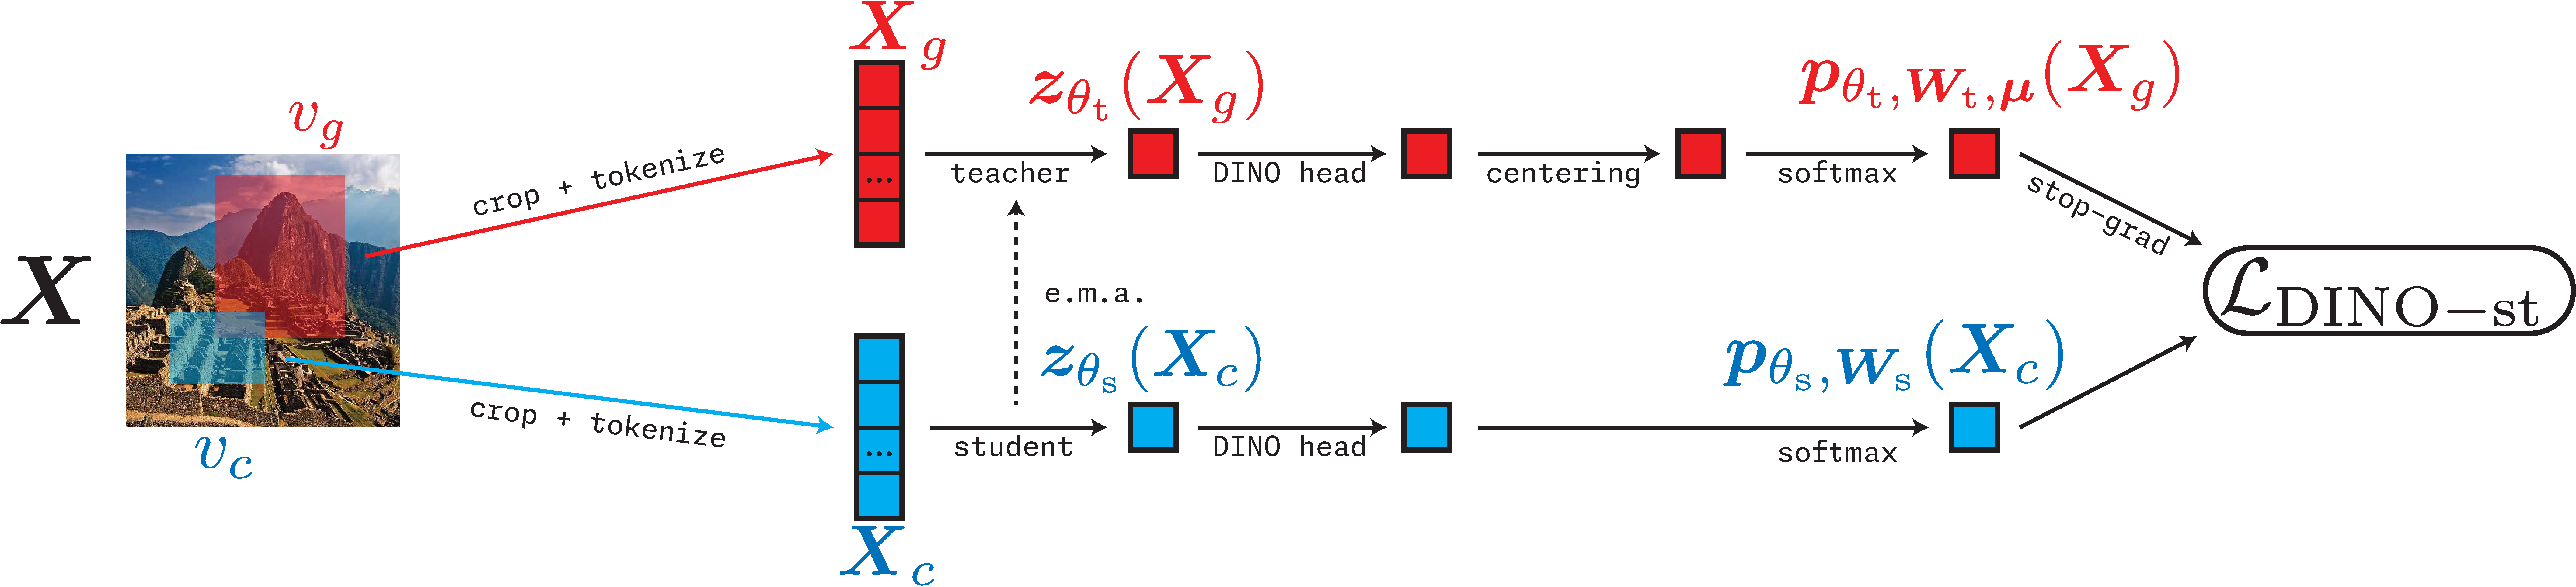
\includegraphics[width=\textwidth]{\toplevelprefix/chapters/chapter7/figs/dino_pipeline.pdf}
    \caption{\small \textbf{The DINO pipeline.} Student features and teacher features are computed for each input. The objective attempts to align the student features with the teacher features by projecting both sets of features into a high-dimensional probability simplex and computing a cross-entropy loss. Notably, because of the ``stop-grad'', the gradient is only computed w.r.t.~the \textit{student parameters' outputs}.}
    \label{fig:dino_pipeline}
\end{figure}

\paragraph{Optimizing DINO.} We have a loss function and an architecture, so we now discuss the optimization strategy. The optimization strategy for DINO uses \textit{two sets of weights for the same architecture}: \textit{student} weights \(\theta_{\student}\) and \textit{teacher} weights \(\theta_{\teacher}\). These correspond to two different neural networks, called the teacher network and student network, with the same architecture. The teacher network encodes all global views, while the student network encodes all ``other'' views. The goal of the loss is to distill teacher outputs into the student model. Namely, we train on the loss \(\cL_{\dino{}-\student\teacher}\):
\begin{equation}\label{eq:dino_loss_teacherstudent}
    \cL_{\dino{}-\student\teacher}(\theta_{\student}, \theta_{\teacher}, \vW_{\student}, \vW_{\teacher}, \vmu) \doteq \Ex[d_{\CE}(\vp_{\theta_{\teacher}, \vW_{\teacher}, \vmu}(\vX_{g}), \vp_{\theta_{\student}, \vW_{\student}}(\vX_{c}))].
\end{equation}
Now, we can fully describe the overall pipeline of DINO, depicted in \Cref{fig:dino_pipeline}.

While it is easy to reason about \eqref{eq:dino_loss_teacherstudent}, it is impossible in practice to implement optimization algorithms such as gradient descent with a loss given by \(\cL_{\dino{}-\student\teacher}\). This is because the expectations in the loss are impossible to evaluate, much less to take the gradient of. In this extremely frequent case, we approximate the expectation via finite samples. That is, at each timestep \(k\) we:
\begin{itemize}
    \item Subsample \(B\) data points from our dataset \(\{\vX_{1}^{(k)}, \dots, \vX_{B}^{(k)}\} \subset \cI\).
    \item For each data point \(\vX_{b}^{(k)}\), sample \(M_{\glo}\) global views \(v_{b, g}^{(k), i}\) and \(M_{\loc}\) local views \(v_{b, \ell}^{(k), i}\). Apply the views to \(\vX_{b}^{(k)}\) to obtain \(\vX_{b, g}^{(k), i} \doteq v_{b, g}^{(k), i}(\vX_{b}^{(k)})\) and \(\vX_{b, \ell}^{(k), i} \doteq v_{b, \ell}^{(k), i}(\vX_{b}^{(k)})\).
    \item For each \textit{local} view \(\vX_{b, \ell}^{(k), i}\), compute the following quantities:
    \begin{equation}
        \vz_{\theta_{\student}}(\vX_{b, \ell}^{(k), i}) \doteq (f_{\theta_{\student}}^{\ext} \circ f_{\theta_{\student}})(\vX_{b, \ell}^{(k), i}), \qquad \vp_{\theta_{\student}, \vW_{\student}}(\vX_{b, \ell}^{(k), i}) \doteq h_{\vW_{\student}, \vzero_{m}}(\vz_{\theta_{\student}}(\vX_{b, \ell}^{(k), i}(\theta)))
    \end{equation}
    and for each \textit{global} view \(\vX_{b, g}^{(k), i}\), compute the following quantities (by an abuse of notation):
    \begin{align}
        &\vz_{\theta_{\student}}(\vX_{b, g}^{(k), i}) \doteq (f_{\theta_{\student}}^{\ext} \circ f_{\theta_{\student}})(\vX_{b, g}^{(k), i}), \qquad \vp_{\theta_{\student}, \vW_{\student}}(\vX_{b, g}^{(k), i}) \doteq h_{\vW_{\student}, \vzero_{m}}(\vz_{\theta_{\student}}(\vX_{b, g}^{(k), i})), \\
        &\vz_{\theta_{\teacher}}(\vX_{b, g}^{(k), i}) \doteq (f_{\theta_{\teacher}}^{\ext} \circ f_{\theta_{\teacher}})(\vX_{b, g}^{(k), i}), \qquad \vp_{\theta_{\teacher}, \vW_{\teacher}, \vmu}(\vX_{b, g}^{(k), i}) \doteq h_{\vW_{\teacher}, \vmu}(\vZ_{\theta_{\teacher}}(\vX_{b, g}^{(k), i})).
    \end{align}
    \item Compute the \textit{surrogate, approximate loss} \(\hat{\cL}_{\dino-\student\teacher}^{(k)}\), defined as follows: 
    \begin{align}\label{eq:dino_loss_teacherstudent_empirical}
        &\hat{\cL}_{\dino{}-\student\teacher}^{(k)}(\theta_{\student}, \theta_{\teacher}, \vW_{\student}, \vW_{\teacher}, \vmu) \doteq
        \frac{1}{BM_{\glo}(M_{\glo} + M_{\loc} - 1)}\sum_{b = 1}^{B}\sum_{i = 1}^{M_{\glo}}\\
        &\Bigg[\sum_{j = 1}^{M_{\loc}}d_{\CE}(\vp_{\theta_{\teacher}, \vW_{\teacher}, \vmu}(\vX_{b, g}^{(k), i}), \vp_{\theta_{\student}, \vW_{\student}}(\vX_{b, \ell}^{(k), j})) + \sum_{\substack{j = 1 \\ j \neq i}}^{M_{\glo}}d_{\CE}(\vp_{\theta_{\teacher}, \vW_{\teacher}, \vmu}(\vX_{b, g}^{(k), i}), \vp_{\theta_{\student}, \vW_{\student}}(\vX_{b, g}^{(k), j}))\Bigg]\nonumber
    \end{align}
    as well as its gradients with respect to \(\theta_{\student}\) and \(\vW_{\student}\), which should be computed under the assumption that \(\theta_{\teacher}\), \(\vW_{\teacher}\), and \(\vmu\) are constants --- namely that they are \textit{detached from the computational graph} and not dependent on \(\theta_{\student}\) and \(\vW_{\student}\).
    \item Update the student parameters \(\theta_{\student}\) and \(\vW_{\student}\) via an iterative gradient-based optimization algorithm, and update \(\theta_{\teacher}\), \(\vW_{\teacher}\), and \(\vmu\) via exponential moving averages with decay parameters \(\nu^{(k)}\), \(\nu^{(k)}\), and \(\rho^{(k)}\) respectively, i.e., 
    \begin{align}
        (\theta_{\student}^{(k + 1)}, \vW_{\student}^{(k + 1)})
        &= \textsc{OptUpdate}^{(k)}(\theta_{\student}^{(k)}, \vW_{\student}^{(k)}; \nabla_{(\theta_{\student}, \vW_{\student})}\hat{\cL}_{\dino-\student\teacher}^{(k)}) \\
        \theta_{\teacher}^{(k + 1)}
        &= \nu^{(k)}\theta_{\teacher}^{(k)} + (1 - \nu^{(k)})\theta_{\student}^{(k + 1)} \\
        \vW_{\teacher}^{(k + 1)}
        &= \nu^{(k)}\vW_{\teacher}^{(k)} + (1 - \nu^{(k)})\vW_{\student}^{(k + 1)} \\
        \vmu^{(k + 1)}
        &= \rho^{(k)}\vmu^{(k)} + (1 - \rho^{(k)})\cdot\frac{1}{BM_{\glo}}\sum_{b = 1}^{B}\sum_{i = 1}^{M_{\glo}}\vW^{(k)}\vz_{\theta_{\teacher}}(\vX_{b, g}^{(k), i}),
    \end{align}
    For example, if the chosen optimization algorithm were stochastic gradient descent, we would have the update \(\theta_{\student}^{(k + 1)} \doteq \theta_{\student}^{(k)} - \delta^{(k)}\nabla_{\theta_{\student}}\hat{\cL}_{\dino{}-\student\teacher}^{(k)}\), and so on.
\end{itemize}
Notice that the optimization procedure is rather irregular: although all four parameters change at each iteration, only two of them are directly updated from a gradient-based method. The other two are updated from exponential moving averages, and indeed treated as constants when computing any gradients. After training, we discard the student weights and use the teacher weights for our trained network \(f\), as this exponentially moving average has been empirically shown to stabilize the resulting model (this idea is known as Polyak averaging or iterate averaging). 

The way that \(\nu\) and \(\rho\) change over the optimization trajectory (i.e., the functions \(k \mapsto \nu^{(k)}\) and \(k \mapsto \rho^{(k)}\)) are hyperparameters or design decisions, with \(\nu^{(1)} < 1\) and \(\lim_{k \to \infty}\nu^{(k)} = 1\) usually, and similar for \(\rho\). The temperature hyperparameter \(\tau\), used in the DINO head \(h_{\vW, \vmu}\), also changes over the optimization trajectory (though this dependence is not explicitly notated).

Using the surrogate (``empirical'') loss transforms our intractable optimization problem, as in optimizing the loss in \eqref{eq:dino_loss_teacherstudent}, into a tractable stochastic optimization problem which is run to train essentially every deep learning model in the world. This conversion is extremely natural once you have seen some examples, and we will hopefully give these examples throughout the chapter. 

\begin{figure}
    \centering 
    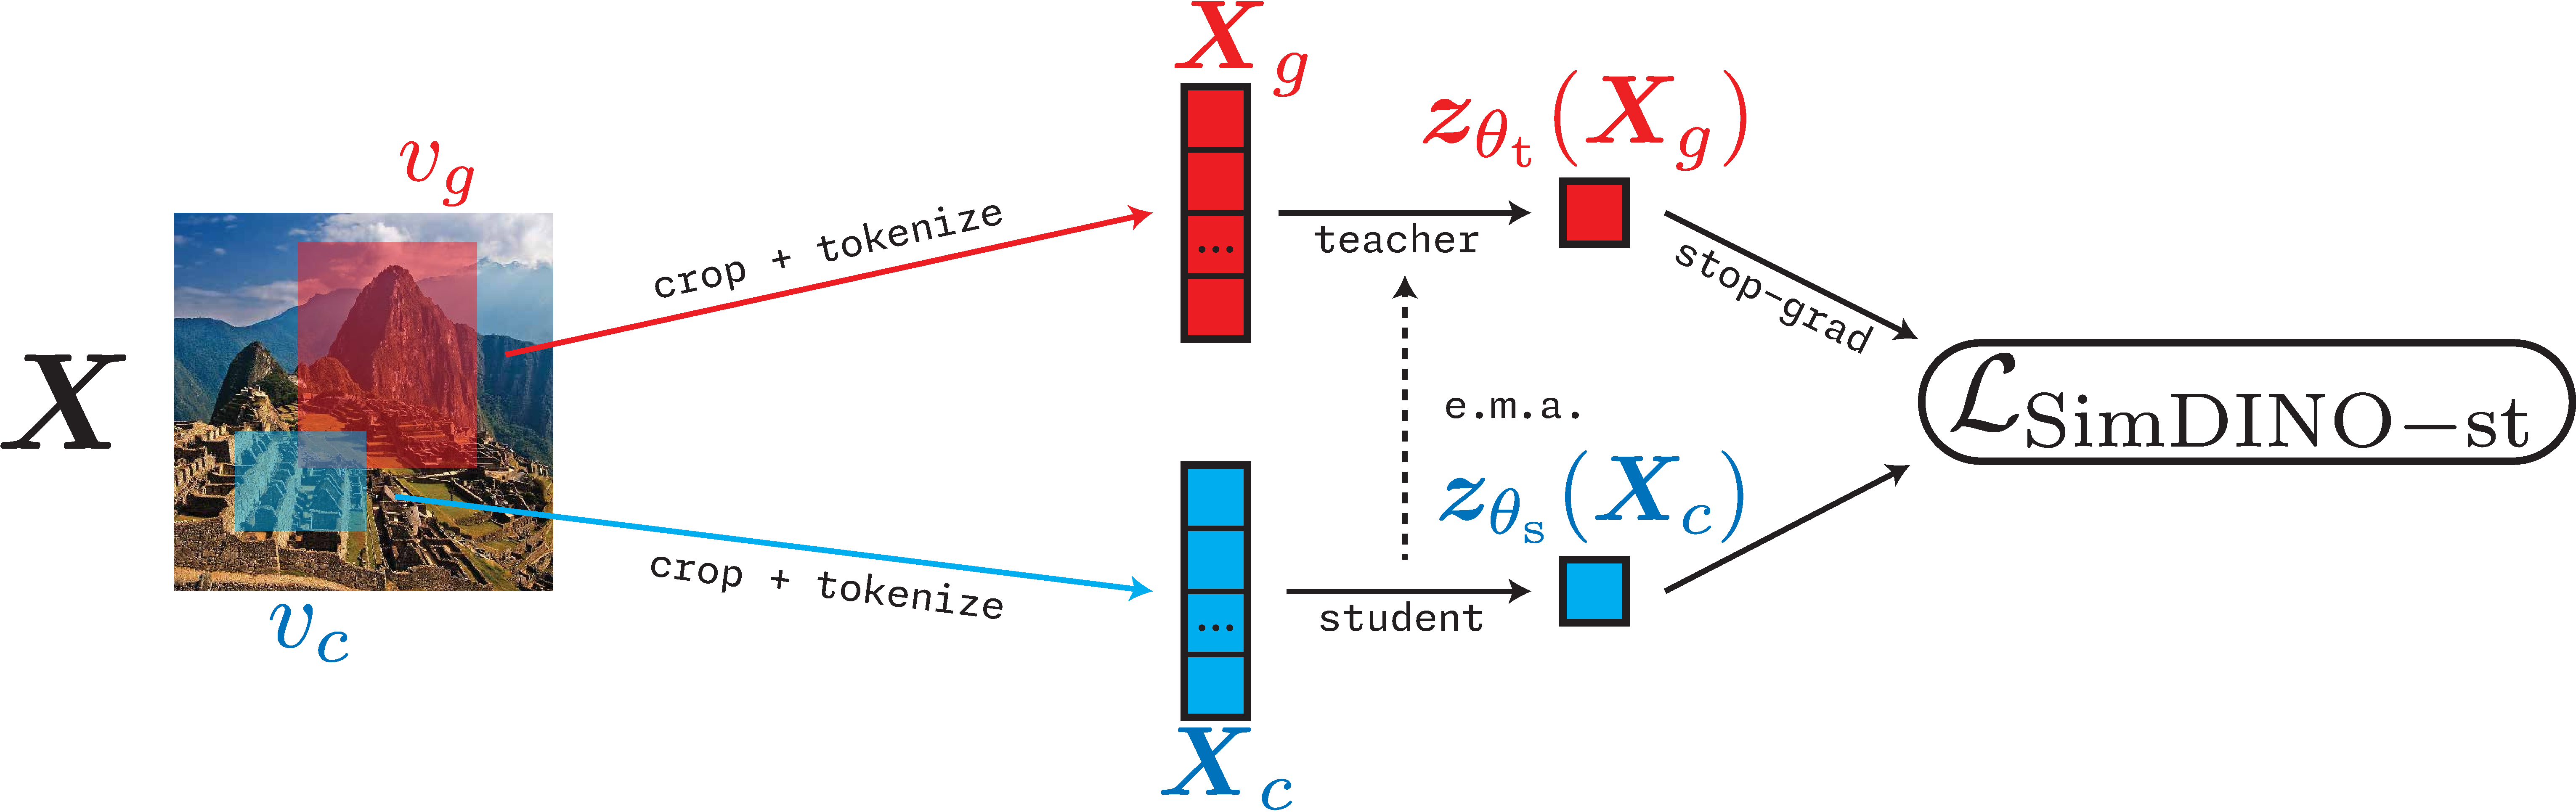
\includegraphics[width=0.7\textwidth]{\toplevelprefix/chapters/chapter7/figs/simdino_pipeline.pdf}
    \caption{\small\textbf{The SimDINO pipeline.} Here, in contrast to the DINO pipeline in \Cref{fig:dino_pipeline}, the loss is computed directly on the features without need of further manipulation. This shaves off several large matrices' worth of parameters and simplifies the pipeline, simultaneously making it more stable to train.}\label{fig:simdino_pipeline}
\end{figure}

\paragraph{Optimizing SimDINO.} The simplified DINO population-level objective is very similar in spirit but much simpler in execution, i.e.,
\begin{equation}\label{eq:simdino_loss_teacherstudent}
    \cL_{\simdino-\student\teacher}(\theta_{\student}, \theta_{\teacher}) \doteq
    \Ex\rs{d_{\ell^{2}}(\vz_{\theta_{\teacher}}(\vX_{g}),
    \vz_{\theta_{\student}}(\vX_{c}))} - \frac{\gamma}{2}\log\det\rp{\vI + \frac{d}{\eps^{2}}\Cov(\vz_{\theta_{\student}}(\vX_{g})))}.
\end{equation}
Thus, as elaborated in \Cref{fig:simdino_pipeline}, the SimDINO pipeline is strictly simpler than the DINO pipeline. We can use a simpler version of the DINO training pipeline to optimize SimDINO. At each timestep \(k\), we:
\begin{itemize}
    \item Subsample \(B\) data points from our dataset \(\{\vX_{1}^{(k)}, \dots, \vX_{B}^{(k)}\} \subset \cI\).
    \item For each data point \(\vX_{b}^{(k)}\), sample \(M_{\glo}\) global views \(v_{b, g}^{(k), i}\) and \(M_{\loc}\) local views \(v_{b, \ell}^{(k), i}\). Apply the views to \(\vX_{b}^{(k)}\) to obtain \(\vX_{b, g}^{(k), i} \doteq v_{b, g}^{(k), i}(\vX_{b}^{(k)})\) and \(\vX_{b, \ell}^{(k), i} \doteq v_{b, \ell}^{(k), i}(\vX_{b}^{(k)})\).
    \item For each \textit{local} view \(\vX_{b, \ell}^{(k), i}\) compute \(\vz_{\theta_{\student}}(\vX_{b, \ell}^{(k), i}) \doteq (f_{\theta_{\student}}^{\ext} \circ f_{\theta_{\student}})(\vX_{b, \ell}^{(k), i})\). For each \textit{global} view \(\vX_{b, g}^{(k), i}\) compute \(\vz_{\theta_{\student}}(\vX_{b, g}^{(k), i}) \doteq (f_{\theta_{\student}}^{\ext} \circ f_{\theta_{\student}})(\vX_{b, g}^{(k), i})\) and \(\vz_{\theta_{\teacher}}(\vX_{b, g}^{(k), i}) \doteq (f_{\theta_{\teacher}}^{\ext} \circ f_{\theta_{\teacher}})(\vX_{b, g}^{(k), i})\).
    \item Compute the \textit{surrogate, approximate loss} \(\hat{\cL}_{\simdino-\student\teacher}^{(k)}\), defined as follows: 
    \begin{align}\label{eq:simdino_loss_teacherstudent_empirical}
        &\hat{\cL}_{\simdino{}-\student\teacher}^{(k)}(\theta_{\student}, \theta_{\teacher}) \doteq
        \frac{1}{BM_{\glo}(M_{\glo} + M_{\loc} - 1)}\sum_{b = 1}^{B}\sum_{i = 1}^{M_{\glo}}\Bigg[\sum_{j = 1}^{M_{\loc}}d_{\ell^{2}}(\vz_{\theta_{\teacher}}(\vX_{b, g}^{(k), i}), \vz_{\theta_{\student}}(\vX_{b, \ell}^{(k), j})) \\ 
        &\qquad \qquad + \sum_{j = 1}^{M_{\glo}}d_{\ell^{2}}(\vz_{\theta_{\teacher}}(\vX_{b, g}^{(k), i}), \vz_{\theta_{\student}}(\vX_{b, g}^{(k), j}))\Bigg] - \frac{\gamma}{M_{\glo}}\sum_{i = 1}^{M_{\glo}}R_{\eps}([\vz_{\theta_{\student}}(\vX_{1, g}^{(k), i}), \dots, \vz_{\theta_{\student}}(\vX_{B, g}^{(k), i})])\nonumber
    \end{align}
    where \(R_{\eps}\) is the Gaussian coding rate estimated on finite samples, described in \Cref{ch:representation}. The gradient of \(\hat{\cL}_{\simdino-\student\teacher}^{(k)}\) with respect to \(\theta_{\student}\) should (again) be computed, under the assumption that \(\theta_{\teacher}\) is constant.
    \item Update the student parameters \(\theta_{\student}\) via an iterative gradient-based optimization algorithm, and update \(\theta_{\teacher}\) via an exponential moving average with decay parameter \(\nu^{(k)}\), i.e., 
    \begin{align}
        \theta_{\student}^{(k + 1)}
        &= \textsc{OptUpdate}^{(k)}(\theta_{\student}^{(k)}; \nabla_{\theta_{\student}}\hat{\cL}_{\simdino-\student\teacher}^{(k)}) \\
        \theta_{\teacher}^{(k + 1)}
        &= \nu^{(k)}\theta_{\teacher}^{(k)} + (1 - \nu^{(k)})\theta_{\student}^{(k + 1)}.
    \end{align}
\end{itemize}
Again, we re-iterate that the gradient is only taken w.r.t.~\(\theta_{\student}\), treating \(\theta_{\teacher}\) as a constant. Here, note that while the choice of \(\nu\) is still a design decision, the hyperparameters \(\rho\) and \(\tau\) are removed.


\subsection{Evaluation Methodology}\label{sub:contrastive_learning_evals}
There are several ways to evaluate a trained transformer model. We highlight two in this section. Let us define the \textit{center crop} view \(v_{\cc} \colon \cI \to \cI\) which is a \textit{deterministic resized crop}:
\begin{itemize}
    \item it resizes the image so that the shortest edge is of size \(S_{\rsz}\) (similar to random resized crops with area percentage parameter \(1\));
    \item then it takes the \textit{center} \(S_{\cc} \times S_{\cc}\) crop;
\end{itemize}
so that the final shape is \((C, S_{\cc}, S_{\cc})\). Notice that the view \(v_{\cc}\) is completely deterministic given an input. For an input \(\vX\), we write \(\vX_{\cc} \doteq v_{\cc}(\vX)\). Here \(S_{\cc} \leq S_{\rsz}\).


\paragraph{Linear probing.}

The first, and most architecture-agnostic, way to evaluate an encoder model \(\vX \mapsto \vz_{\theta}(\vX)\) is to employ \textit{linear probing}. Linear probing is, in a sentence, running logistic regression on the aggregate features computed by the encoder. This tells us how much semantic information exists in the representations, as well as how easily this information can be extracted. (That is: to what extent do the features of images with different semantics live on different subspaces of the feature space?)

More formally, let us suppose that we want to evaluate the quality and faithfulness of the features of the encoder on image-label data \((\vX, \vy)\), where there are \(N_{\cls}\) classes and \(\vy \in \{0, 1\}^{N_{\cls}}\) is a ``one-hot encoding'' (namely, zeros in all positions except a \(1\) in the \(i\)th position if \(\vX\) is in the \(i\)th class). One way to do this is to solve the logistic regression problem 
\begin{equation}\label{eq:linear_probing}
    \min_{\vW \in \R^{N_{\cls} \times d}}\Ex[\CE(\vy, \vW \vz_{\theta}(\vX_{\cc}))].
\end{equation}
More practically, if we have labeled data \(\{(\vX_{b}, \vy_{b})\}_{b = 1}^{B}\), we can solve the \textit{empirical} logistic regression problem (akin to \eqref{eq:dino_loss_teacherstudent} vs.~\eqref{eq:dino_loss_teacherstudent_empirical}) given by 
\begin{equation}\label{eq:linear_probing_empirical}
    \min_{\vW \in \R^{N_{\cls} \times d}}\frac{1}{B}\sum_{b = 1}^{B}\CE(\vy_{b}, \vW \vz_{\theta}(\vX_{b, \cc})).
\end{equation}
This problem is a convex optimization problem in \(\vW\), and thus can be solved efficiently via (stochastic) gradient descent or a litany of other algorithms. This linear probe, together with the encoder, may be used as a classifier, and we can evaluate the classification accuracy. The usual practice is to train the model first on a large dataset (such as ImageNet-1K), then train the linear probe on a dataset (such as the training dataset of CIFAR-10), and evaluate it on a third (``holdout'') dataset which is drawn from the same distribution as the second one (such as the evaluation dataset of CIFAR-10).

\paragraph{\(k\)-nearest neighbors.}  We can also evaluate the performance of the features on classification tasks \textit{without needing to explicitly train a classifier} by using the \(k\)-nearest neighbor algorithm to get an average predicted label. Namely, given a dataset \(\{\vz_{b}\}_{b = 1}^{B} \subseteq \R^{d}\), define the \(k\)-nearest neighbors of another point \(\vz \in \R^{d}\) as \(\operatorname{NN}_{k}(\vz, \{\vz_{b}\}_{b = 1}^{B})\). Using this notation, we can compute the predicted label \(\hat{\vy}_{\theta}(\vX \mid \{(\vX_{b}, \vy_{b})\}_{b = 1}^{B})\) as 
\begin{equation}
    \hat{\vy}_{\theta}(\vX \mid \{(\vX_{b}, \vy_{b})\}_{b = 1}^{B}) = \vone(i^{\star}) \quad \text{where} \quad i^{\star} \doteq \argmax_{i \in [Q]}\sum_{b = 1}^{B}\vy_{b}\indvar[\vz_{\theta}(\vX_{\cc, b}) \in \operatorname{NN}_{k}(\vz_{\theta}(\vX_{\cc}))].
\end{equation}
Here, \(\vone(i) \in \Delta_{N_{\cls}}\) is (by an abuse of notation, cf.~indicator variables) the one-hot probability vector supported at \(i\), i.e., \(1\) in the \(i\)th coordinate and \(0\) elsewhere. That is, this procedure takes the most common label among the \(k\) nearest points in feature space. The \(k\)-nearest neighbor classification accuracy is just the accuracy of this predicted label, namely,
\begin{equation}
    \Ex_{\vX, \vy}[\indvar(\hat{\vy}_{\theta}(\vX \mid \{(\vX_{b}, \vy_{b})\}_{b = 1}^{B}) = \vy)]
\end{equation}
or more commonly its corresponding empirical version, where \((\vX, \vy)\) ranges over a finite dataset (\textit{not} the existing samples \((\vX_{b}, \vy_{b})\) which are used for the \(k\) neighbors).

\paragraph{Fidelity of the attention maps.}

Another way to check the performance of the representations, for a transformer-based encoder, is to examine the fidelity of the attention maps \(\vA^{L, k} \in \R^{n \times n}\) as defined in \Cref{eq:attention_map}, at the last layer \(L\), and given by the following pipeline:
\begin{align}
    \vX \mapsto \cdots \mapsto \vZ^{L - 1} = [\underbrace{\vz_{1}^{L - 1}}_{\text{class token}}, \underbrace{\vz_{2}^{L - 1} \dots, \vz_{n}^{L - 1}}_{\text{patch tokens}}] \mapsto \vA^{k, L} = \mat{\vA_{1, 1}^{k, L} & \vA_{1, 2:}^{k, L} \\ \vA_{2:, 1}^{k, L} & \vA_{2:, 2:}^{k, L}}.
\end{align}
In particular, we examine what the attention maps for a given input reveal about the salient objects in the input image, i.e., which parts of the image provide the most globally-relevant information to the class token. One particular way to do this is to examine the component of the attention map where the class token is extracted as the query and removed from the value matrix, i.e., \(\vA_{2:, 1}^{k, L} \in \R^{1 \times (n - 1)} = \R^{1 \times N}\) or its transpose \(\va^{k, L} = (\vA_{2:, 1}^{k, L})^{\top} \in \R^{N}\). Notice that this vector \(\va^{k, L}\), which we label as the ``\textit{saliency vector} at the \(k\)th attention head at layer \(L\),'' has a value for every patch, \(1, \dots, N\), and we use this value to describe how relevant each patch is toward the global information. In particular for visualization's sake we create a new image where each patch is replaced by its corresponding value in the saliency vector, showcasing the contribution of each patch; we call this image the ``\textit{saliency map} at the \(k\)th attention head at layer \(L\)''. To visualize the total relevance of each patch toward the global information across all heads, we can average the saliency vector, i.e., \(\tilde{\va}^{L} \doteq \frac{1}{K}\sum_{k = 1}^{K}\va^{k, L}\) and expand into the \textit{average saliency map}. The average saliency maps should highlight the relevant parts of the input image.


\paragraph{Object detection and segmentation.}

We can evaluate how the representations capture the fine-grained (i.e., smaller or more detailed) properties of the input by using them for \textit{semantic segmentation}. Roughly, this means that we use the features to construct bounding boxes for all objects in the input. There are several ways to do this, and several ways to score the resulting bounding boxes compared to ground truth. Each combination of methods corresponds to a particular segmentation metric. We do not formally describe them here as they are not particularly insightful, but the DINO paper \citep{caron2021emerging} and DINOv2 paper \citep{oquab2023dinov2} contain references to all metrics that are used in practice.

\subsection{Experimental Setup and Results} \label{sub:contrastive_learning_experiment_results}

Since SimDINO is directly built upon DINO, we compare the optimal settings for DINO as given by their original paper \citep{caron2021emerging} with the same settings applied to SimDINO for a fair comparison. 

\paragraph{Objective function.} We use \(10\) local views (i.e., \(M_{\loc} = 10\)) of resolution \(96 \times 96\) (i.e., \(S_{\loc} = 96\)) and \(2\) global views (i.e., \(M_{\glo} = 2\)) of resolution \(224 \times 224\) (i.e., \(S_{\glo} = 224\)) for all experiments. The corresponding portions of the original images cropped for local and global views are \(p_{\loc} \in [\frac{1}{20}, \frac{3}{10}]\) and \(p_{\glo} \in [\frac{3}{10}, 1]\) (chosen randomly per-view). The smaller edge size within the resized crops is \(S_{\rsz} = 256\), and the center crop (evaluation) view edge size is \(S_{\cc} = 224\). All of these settings apply to both DINO and SimDINO.

\paragraph{Model architecture.} For all inputs, we set the patch size to be \(16 \times 16\) (namely, \(P_{H} = P_{W} = 16\)). We use the small, base, and large models of the ViT \citep{dosovitskiy2020image} architecture as the embedding and backbone. The feature extractor is a three-layer MLP with a hidden size of \(2048\) and an output dimension of \(256\), followed by an \(\ell^{2}\)-normalization, as specified in \Cref{sub:contrastive_learning_architecture}. For DINO architectures (i.e., not SimDINO architectures), the DINO head \(\vW\) is a matrix in \(\R^{65536 \times 256}\), and the parameter \(\vmu\) is a vector in \(\R^{65536}\). 

\paragraph{Datasets and optimization.} For pre-training, both our DINO reproduction and SimDINO use the ImageNet-1K dataset across all methods. We use AdamW \citep{Loshchilov2017DecoupledWD} as the optimizer, which is a very standard choice. We follow the following hyperparameter recommendations:
\begin{itemize}
    \item The batch size is \(B = 1024\).
    \item The learning rate (for AdamW and the student model) has ``base'' value \(2 \times 10^{-3}\). In the first \(10\) epochs the learning rate linearly increases from \(0\) to the base value (i.e., at the \(i\)th epoch the learning rate is \((i/10) \cdot 2 \times 10^{-3}\), for \(1 \leq i \leq 10\)). Then over the next \(90\) epochs the learning rate decays via a so-called \textit{cosine schedule} back down to \(0\). The definition of a cosine schedule is given in many places, including \href{https://pytorch.org/docs/stable/generated/torch.optim.lr_scheduler.CosineAnnealingLR.html}{PyTorch documentation}, and it is commonly used when training deep vision models.
    \item The weight decay (the W in AdamW) follows a cosine schedule from 0.04 to \(0.4\) over training.
    \item The EMA rate \(\nu\) follows a cosine schedule from \(0.996\) to \(1.0\) over training. Specifically for DINO, the centering EMA rate \(\rho\) is fixed at \(0.9\).
    \item Specifically for DINO, the teacher temperature \(\tau_{\teacher}\) is fixed at \(0.1\), while the student temperature \(\tau_{\student}\) linearly increases from \(0.04\) to \(0.07\) during the first \(30\) epochs and is fixed at \(0.07\) thereafter.
\end{itemize}
We use some (essentially information-preserving) data augmentations, such as flips, color jittering, Gaussian blur, and solarization, for each seen image during training, before taking the local and global views. The exact hyperparameters governing these are not listed here, but are referenced in the DINO paper \citep{caron2021emerging}.

For linear probing, the linear probe is usually trained using the AdamW optimizer with learning rate \(2 \times 10^{-4}\), weight decay \(0.01\), and batch size \(512\), but these are often modified on a case-by-case basis to minimize the loss.


\begin{table}
    \centering
    \begin{tabular}{@{}lcccc@{}} %
        \toprule
        Method & Model & Epochs & 20-NN & Linear Probing 
        \\
        \midrule 
        DINO & ViT-B & 100 & 72.9 & 76.3 \\
        SimDINO & ViT-B & 100 & \bf 74.9 & \bf 77.3 \\
        DINO & ViT-L & 100 & -- & -- \\
        SimDINO & ViT-L & 100 & \bf 75.6 & \bf 77.4 \\
        \midrule
        \color{gray} SwAV & \color{gray} ViT-S & \color{gray} 800 & \color{gray} 66.3 & \color{gray} 73.5 \\
        \color{gray} MoCov3 & \color{gray} ViT-B & \color{gray} 300  & \color{gray} -- & \color{gray} 76.7 \\
        \bottomrule
    \end{tabular}
    \caption{\small\textbf{Classification performance} on hold-out test data for DINO and SimDINO, using both \(k\)-nearest neighbor accuracy (\(k = 20\)) and linear probing. At the same number of iterations (\(100\)), SimDINO is clearly better in terms of performance, and is more stable (the DINO training running on ViT-L backbone with the provided settings has very unstable optimization and obtains NaN loss in short order). We also compare to other standout methods, namely SwAV and MoCov3, which DINO was built on.}
    \label{tab:dino_imagenet_linear_probing}
\end{table}

\begin{figure}
    \centering 
    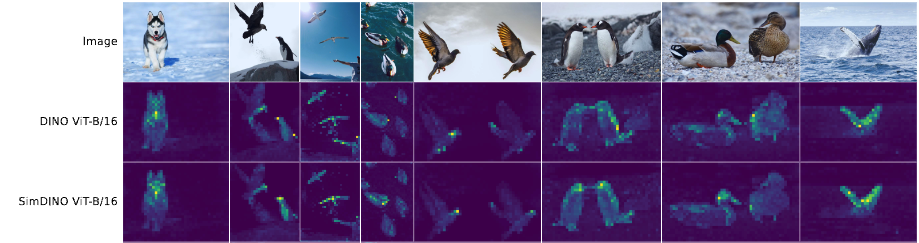
\includegraphics[width=\textwidth]{\toplevelprefix/chapters/chapter7/figs/dino_attention_maps.png}
    \caption{\small\textbf{A qualitative comparison of saliency maps} generated by DINO \textit{(middle row)} and by SimDINO \textit{(bottom row)}. For each image, we compute and display the average saliency map in the last layer \(L\). The saliency maps are similar across models, meaning that all models converge to a similar notion of what objects are important. Note that although \(X_{\evaluation}\) is a square image, it is interpolated back into rectangular shape to make this visualization.}
    \label{fig:dino_attention_maps_saliency}
\end{figure}

\begin{table}
    \centering 
    \begin{tabular}{@{}llcccccccc@{}}
        \toprule
         &  & \multicolumn{3}{c}{Detection $\uparrow$} &  \multicolumn{3}{c}{Segmentation $\uparrow$} \\ 
        Method & Model & AP$_{50}$  & AP$_{75}$ & AP & AP$_{50}$ & AP$_{75}$ & AP  \\ 
        \midrule
        SimDINO &ViT-L/16 &\bf 5.4 &1.9 &2.4 &4.5 &1.4 &1.9 \\
        SimDINO &ViT-B/16 &5.2 & \bf 2.0 & \bf 2.5 & \bf4.7 & \bf 1.5 & \bf 2.0 \\
        DINO &ViT-B/16 &3.9 &1.5 &1.8 &3.1 &1.0 &1.4 \\
        \midrule
        \color{gray} DINO & \color{gray} ViT-B/8 & \color{gray}5.1 & \color{gray}2.3 & \color{gray}2.5 & \color{gray}4.1 & \color{gray}1.3 & \color{gray}1.8 \\
        \bottomrule
    \end{tabular}
    \caption{\small\textbf{Segmentation performance} of pre-trained DINO and SimDINO models on COCO val2017 \citep{lin2014microsoft}, a segmentation dataset which contains object location metadata. We do not train on COCO, merely using the pre-trained embedding and backbone, and the bounding boxes are extracted from the features via a method called MaskCut \citep{wang2023cut}. Nevertheless, SimDINO surpasses DINO at object detection and segmentation under fair comparison, and even surpasses DINO with smaller patch size (side length \(8\) instead of \(16\)). Smaller patch sizes are known to help performance, especially with detection and segmentation tasks, so this result is quite surprising and encouraging.}
    \label{tab:dino_segmentation}
\end{table}

\paragraph{Evaluation results.} In terms of downstream classification performance, we obtain the performance in \Cref{tab:dino_imagenet_linear_probing}. We observe that the performance of SimDINO is much higher than that of DINO under fair comparison. Also, it is much more stable: the prescribed settings of DINO cannot train a ViT-L(arge) model. On the other hand, \Cref{fig:dino_attention_maps_saliency} shows visualizations of the average saliency maps in DINO and our simplified DINO, observing that the saliency maps look quite similar across models, indicating that the models learn features which are at least as good at capturing fine-grained details. The segmentation and object detection performances in \Cref{tab:dino_segmentation} confirm this claim quantitatively, where SimDINO features show substantive improvement over those of DINO.



\section{Image Classification}\label{sec:image_classification}

In the previous section, we simplified an overly complex learning objective using our intuition about representation learning through the lens of compression. However, many of the most popular learning procedures are incredibly simple. In these cases, it is difficult to further simplify the objective. Thus, in this and future sections, we will focus on principled ways to modify the \textit{deep network architectures} for a variety of tasks.

Let us first start with arguably the most classical task in machine learning: \textit{image classification}, which is often used as a standard task to evaluate pattern recognition algorithms or deep network architectures. From our discussion of white-box architectures in \Cref{ch:representation}, we only need a semantically meaningful task to learn good representations with white-box architectures. We will validate this idea in this section.

First, the dataset stays largely the same as \Cref{sub:contrastive_learning_data}. Both the training and test data consist of labeled images, i.e., image-label pairs \((\vX, \vy) \in \R^{C \times H \times W} \times \{0, 1\}^{N_{\cls}}\). We still apply various data augmentations (e.g., flips, Gaussian blurring, solarization, etc.) to each sample in each new batch. 

\subsection{Task and Objective} \label{sub:image_classification_objective}

Unlike before, our task is not just to learn a good representation of the data, but also to simultaneously build a classifier. Formally, we have labeled data pairs \((\vX, \vy)\), where \(\vy \in \{0, 1\}^{N_{\cls}}\) is a one-hot vector denoting the class membership of \(\vX\). We consider a deterministic \textit{center crop view} \(v_{\cc}\) of the input data \(\vX\) (cf \Cref{sub:contrastive_learning_objective}). We want to jointly train a feature mapping \((f_{\theta}, f_{\theta}^{\ext})\) and a \textit{classification head} \(h_{\theta}\), defined as follows:
\begin{equation}
    h_{\theta}(\vz) \doteq \softmax(\vW^{\head}\vz + \vb^{\head}), \qquad  \forall \vz \in \R^{d}
\end{equation}
where \((\vW^{\head}, \vb^{\head}) \in \R^{N_{\cls} \times d} \times \R^{N_{\cls}}\) are trainable parameters in the parameter set \(\theta\), such that the map \(\vX_{\cc} \mapsto \vp_{\theta}(\vX_{\cc}) \doteq h_{\theta}(\vz_{\theta}(\vX_{\cc}))\) predicts a smoothed label for the view \(\vX_{\cc} = v_{\cc}(\vX)\) of the input \(\vX\). The learning problem attempts to minimize the distance between \(\vp_{\theta}\) and \(\vy\) measured through cross-entropy:
\begin{equation}\label{eq:classification_ce_loss}
    \min_{\theta}\bc{\cL_{\CE}(\theta) \doteq \Ex[\CE(\vy, \vp_{\theta}(\vX_{\cc}))]}.
\end{equation}


\subsection{The CRATE Architecture}\label{sub:image_classification_architecture}

The architecture that we use is the CRATE architecture, described in some detail in \Cref{ch:representation}. The overall setup is similar to that of the regular transformer in \Cref{sub:contrastive_learning_architecture}, with a few changes. While the embedding step is the same as both DINO and SimDINO in \Cref{sub:contrastive_learning_architecture}, the feature extraction step is the same as SimDINO in \Cref{sub:contrastive_learning_architecture} as it just extracts the feature corresponding to the class token, and the classification head is described in \Cref{sub:image_classification_objective}, the backbone architecture is different. Each layer takes the form
\begin{align}\label{eq:CARTE updates}
    \vZ_{\theta}^{\ell + 1/2}(\vX)
    &= \vZ_{\theta}^{\ell}(\vX) + \MSSA_{\theta}^{\ell}(\LN_{\theta}^{1, \ell}(\vZ_{\theta}^{\ell}(\vX))), \\ 
    \vZ_{\theta}^{\ell + 1}(\vX)
    &= \ISTA_{\theta}^{\ell}(\LN_{\theta}^{2, \ell}(\vZ_{\theta}^{\ell + 1/2}(\vX))),
\end{align}
where the \(\MSSA_{\theta}^{\ell}\) and \(\ISTA_{\theta}^{\ell}\) blocks are as described in \Cref{ch:representation}, namely:
\begin{itemize}
    \item The \(\MSSA\) operator is multi-head-subspace-self-attention, defined as follows:
    \begin{equation}
        \MSSA_{\theta}^{\ell}(\vZ) \doteq \vU_{\out}^{\ell}\mat{\SA([\vU^{1, \ell}]^{\top}\vZ, [\vU^{1, \ell}]^{\top}\vZ, [\vU^{1, \ell}]^{\top}\vZ)\\ \vdots \\ \SA([\vU^{K, \ell}]^{\top}\vZ, [\vU^{K, \ell}]^{\top}\vZ, [\vU^{1, \ell}]^{\top}\vZ)} + \vb_{\out}^{\ell}\vone_{n}^{\top}
    \end{equation}
    where \(\vU^{k, \ell} \in \R^{d \times p}\), \(\vU_{\out}^{\ell} \in \R^{d \times Kp}\), and \(\vb_{\out}^{\ell} \in \R^{d}\) are trainable parameters belonging to the parameter set \(\theta\), and (recall) the self-attention operator \(\SA\) is defined in \eqref{eq:self_attention}.
    \item The \(\ISTA\) operator is the iterative-shrinkage-thresholding-algorithm operator, defined as follows:
    \begin{equation}
        \ISTA_{\theta}^{\ell}(\vZ) \doteq \ReLU(\vZ - \beta (\vD^{\ell})^{\top}(\vD^{\ell}\vZ - \vZ) + \beta\lambda \vone_{d}\vone_{n}^{\top}),
    \end{equation}
    so named because the map \(\vX \mapsto \ReLU(\vX - \beta \vD^{\top}(\vD\vX - \vZ) + \beta  \lambda \vone_{d}\vone_{n}^{\top})\) is one step of the well-established ISTA algorithm to find an element-wise non-negative sparse representation for \(\vZ\) with respect to the complete dictionary \(\vD\) (cf \Cref{sec:dictionary_learning}).
\end{itemize}

We call this architecture CRATE, and a layer of the backbone is depicted in \Cref{fig:crate_backbone}. CRATE models, on top of being interpretable, are generally also highly performant and parameter-efficient. 

\subsection{Optimization} \label{sub:image_classification_optimization}

We train our classifier using a simple end-to-end stochastic optimization procedure, where we subsample data and views, compute the average loss and its gradient over these samples, and use an optimization algorithm to change the parameters. At each timestep \(k\), we:
\begin{itemize}
    \item Subsample \(B\) different labeled samples \(\{(\vX_{b}^{(k)}, \vy_{b}^{(k)})\}_{b = 1}^{B} \subseteq \cI \times \{0, 1\}^{N_{\cls}}\).
    \item For each labeled sample \((\vX_{b}^{(k)}, \vy_{b}^{(k)})\), compute the central crop view \(v_{b, \cc}^{(k)}\) and apply it to \(\vX_{b}^{(k)}\) to get \(\vX_{b, \cc}^{(k)} \doteq v_{b, \cc}^{(k)}(\vX_{b}^{(k)})\).
    \item Compute the predictions \(\vp_{\theta}(\vX_{b, \cc}^{(k)}) \doteq (h_{\theta} \circ f_{\theta}^{\ext} \circ f_{\theta})(\vX_{b, \cc}^{(k)})\).
    \item Form the surrogate stochastic loss 
    \begin{equation}
        \hat{\cL}_{\CE}^{(k)}(\theta) \doteq \frac{1}{B}\sum_{b = 1}^{B}\CE(\vy_{b}^{(k)}, \vp_{\theta}(\vX_{b, \cc}^{(k)})).
    \end{equation}
    \item Compute one step of an optimization algorithm on \(\theta\), giving the following iteration:
    \begin{equation}
        \theta^{(k + 1)} \doteq \textsc{OptUpdate}^{(k)}(\theta^{(k)}; \nabla_{\theta}\hat{\cL}_{\CE}^{(k)}).
    \end{equation}
\end{itemize}


\subsection{Evaluation Methodology} \label{sub:image_classification_evals}

We use the same evaluation procedure as \Cref{sub:contrastive_learning_evals}. To summarize, for all evaluations (as well as training) we use a center crop view \(v_{\cc}\) which reshapes the input image and takes a large central crop of size \((C, S_{\cc}, S_{\cc})\) where \(C\) is the number of channels in the input image. We can then do linear probing, attention map visualization, and detection/segmentation benchmarks, given the output of this view.

\subsection{Experimental Setup and Results}\label{sub:image_classification_experiments}

Since CRATE is directly based on the transformer, we compare the optimal settings for ViT as given by \cite{dosovitskiy2020image,touvron2020training} with the same settings applied to CRATE for a fair comparison.

\paragraph{Model architecture.} The center crop resizes the whole image so that the shorter edge is of size \(256\) (i.e., \(S_{\rsz} = 256\)) before taking a center crop of size \(224 \times 224\) (i.e., \(S_{\cc} = 224\)), both in evaluation and training. We take patch size \(16\) (i.e., \(P_{H} = P_{W} = 16\)). We use the tiny, small, base, and large models of the ViT \cite{dosovitskiy2020image} architecture as the embedding and backbone, swapping out the MHSA and MLP components for MSSA and ISTA, respectively, using the same number of heads and head dimension in the case of MSSA, and therefore reducing the number of training parameters drastically. For CRATE, we set \((\beta, \lambda) = (1, 0.1)\).

\paragraph{Datasets and optimization.} For pre-training, we use the ImageNet-1K dataset. We use the LION optimizer \citep{chen2024symbolic} to pre-train both our ViT replication as well as CRATE. We set the base learning rate as \(2.4 \times 10^{-4}\), the weight decay as \(0.5\), and batch size as \(B = 2048\). Our learning rate schedule increases the learning rate linearly to the base learning rate over the first \(5\) epochs, and decreases to \(0\) using a cosine schedule over the next \(145\) epochs (training all models for \(150\) epochs each). For pre-training, we apply a usual regime of data augmentations (flips, Gaussian blurs, solarization, etc.) to the image data, and also add small noise to the labels (this is called \textit{label smoothing} \citep{muller2019does}).

For linear probing, we use several evaluation datasets such as CIFAR10, Oxford-Flowers, and Oxford-IIT-Pets. We use the AdamW optimizer to train the linear probe, using learning rate \(5 \times 10^{-5}\), weight decay \(0.01\), and batch size \(B = 256\). We also apply the aforementioned data augmentations to the image data.

\begin{table}
    \centering
    \begin{tabular}{@{}lcccc|cc@{}}
    \toprule
    \textbf{Model} & CRATE-T  &  CRATE-S & CRATE-B & CRATE-L & { \color{gray} ViT-T} &  { \color{gray}ViT-S } \\ 
    \midrule
    \midrule
     \# parameters & 6.09M & 13.12M & 22.80M & 77.64M & { \color{gray} 5.72M} & { \color{gray} 22.05M} \\
    \midrule
     ImageNet-1K & 66.7 & 69.2 & 70.8 & 71.3 & { \color{gray} 71.5} & { \color{gray} 72.4} \\
     ImageNet-1K ReaL & 74.0 & 76.0 & 76.5 & 77.4 & { \color{gray} 78.3 } & { \color{gray} 78.4} \\
     CIFAR10 & 95.5 & 96.0 & 96.8 & 97.2 & { \color{gray} 96.6} & { \color{gray} 97.2} \\
     CIFAR100 & 78.9 & 81.0 & 82.7 & 83.6 & { \color{gray} 81.8} & { \color{gray} 83.2}\\
     Oxford Flowers-102 & 84.6 & 87.1 & 88.7 & 88.3 & { \color{gray} 85.1} & { \color{gray} 88.5}\\
     Oxford-IIIT-Pets & 81.4 & 84.9 & 85.3 & 87.4 & { \color{gray} 88.5} & { \color{gray} 88.6} \\
     \bottomrule
    \end{tabular}
    \caption{\small \textbf{Linear probing classification accuracy of CRATE and ViT} on various datasets with different model sizes when the backbone is pre-trained for classification on ImageNet-1K. We observe that given the same model configuration, CRATE has comparable classification performance with a simpler, more principled, and more parameter-efficient design.}
    \label{tab:crate_classification_linear_probing}
\end{table}

\begin{figure}[t]
    \centering
    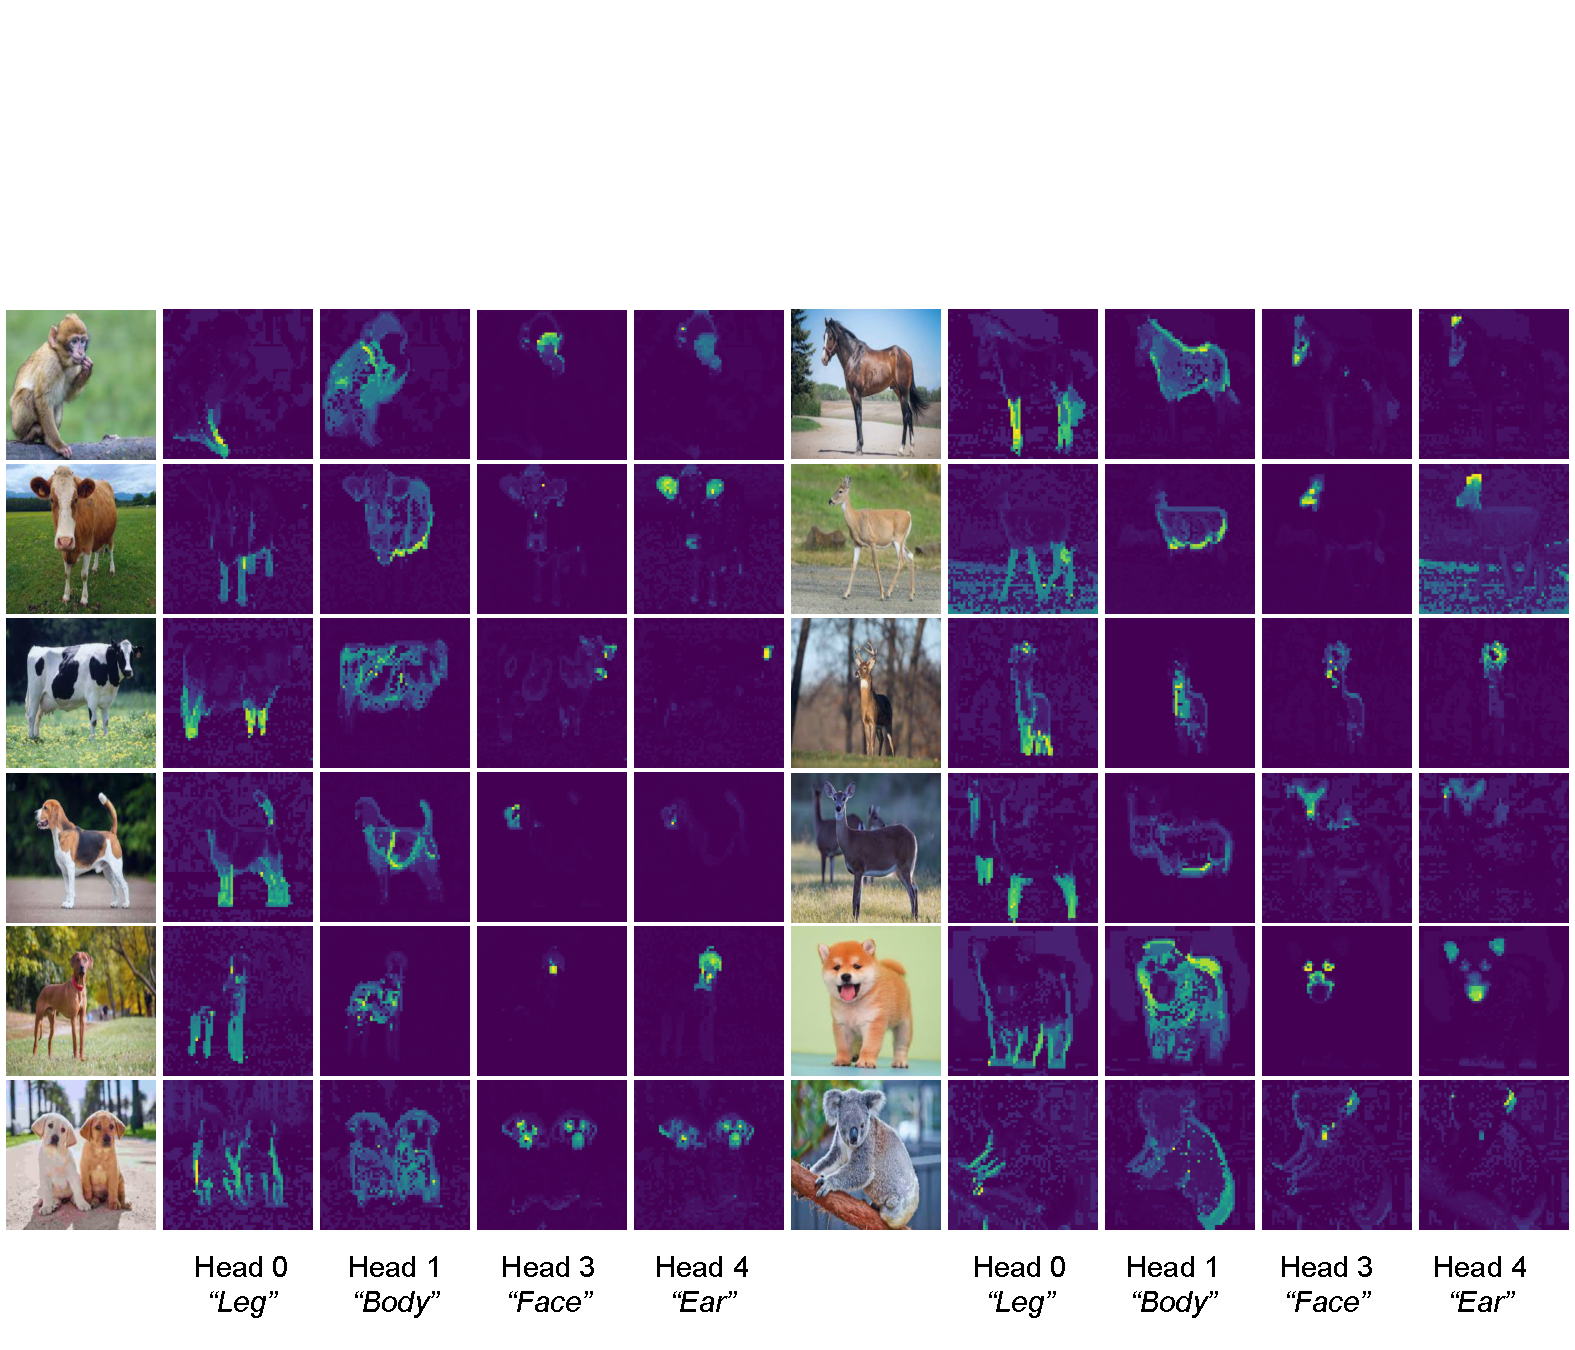
\includegraphics[width=0.8\textwidth]{\toplevelprefix/chapters/chapter7/figs/crate_semantic_heads.pdf}
    \caption{\small\textbf{Interpretable saliency maps in CRATE} with patch size \(8\). When given images with similar properties (perhaps but not necessarily from the same class), the saliency maps corresponding to different attention heads in the last layer each highlight a specific property. One can observe that the average saliency map (not included) then highlights all relevant objects in the image, showing that it uses all fine-grained details of the input image for classification. This is the \textit{first} machine learning system to do this, to the authors' knowledge, much less automatically without training on any segmentation data.}
    \label{fig:crate_semantic_heads}
\end{figure}

\begin{table}
    \centering
    \begin{tabular}{@{}lcccccccc@{}}
    \toprule
     &  \multicolumn{3}{c}{Detection (\(\uparrow\))} &  \multicolumn{3}{c}{Segmentation (\(\uparrow\))} \\ 
    Model & AP$_{50}$ & AP$_{75}$ & AP & AP$_{50}$ & AP$_{75}$ & AP  \\ 
    \midrule
    CRATE-S/8 & \textbf{2.9} & \textbf{1.0} & 1.1 & 1.8 & \textbf{0.7} & 0.8 \\
    CRATE-B/8 & \textbf{2.9} & \textbf{1.0} & \textbf{1.3} & \textbf{2.2} & \textbf{0.7} & \textbf{1.0} \\
    ViT-S/8 & 0.1& 0.1 & 0.0 & 0.0 & 0.0 & 0.0 \\
    ViT-B/8 & 0.8 & 0.2 & 0.4 & 0.7 & 0.5 & 0.4 \\
    \bottomrule
    \end{tabular}
    \caption{\small \textbf{Object detection and fine-grained segmentation via MaskCut on COCO {val2017}~\citep{lin2014microsoft}}. Here all models are trained with patch size \(8\) instead of \(16\). CRATE conclusively performs better than the ViT at detection and segmentation metrics when both are trained using supervised classification.}
    \label{tab:crate_detection_segmentation}
\end{table}


\paragraph{Experiment results.} 

\Cref{tab:crate_classification_linear_probing} demonstrates that CRATE models achieve parity or improvement compared to the popular Vision Transformer (ViT) architecture at similar parameter counts, at least in terms of the linear separability of their features with respect to different classes. In terms of attention map fidelity, \Cref{fig:crate_semantic_heads} demonstrates a truly extraordinary result: without needing to train on any segmentation or object detection data, \textit{not only} do the saliency maps effectively capture all relevant parts of the input image, the saliency maps \textit{self-organize} to each correspond to a discrete set of concepts, even across samples and classes! This is the first system to do this, to the authors' knowledge, and it can do this without using any extra data except for the image classification data. \Cref{tab:crate_detection_segmentation} confirms these qualitative insights quantitatively, showing significant improvement over ViTs trained in the same supervised classification setup.

\section{Causal Language Modeling}\label{sec:clm_text}

We now study \textit{causal language modeling}, a method for training large language models (LLMs). This is the same setup used to train, among many others, GPT-2 and many other language models. 

\subsection{Data} \label{sub:clm_text_data}

The data we will use to investigate the performance of CRATE for language tasks will be OpenWebText (OWT)~\cite{Gokaslan2019OpenWeb}, an open-source reproduction of the unreleased WebText dataset used by OpenAI to train GPT2. Each sample in OWT is a web document, typically sourced from high-quality web pages, blogs, articles, or online discussions, that is written in well-formed natural language. The OpenWebText dataset contains around 8.01M documents of varying lengths, totaling around 41.70GB of text. For evaluation, we will use several datasets, such as WikiText~\cite{merity2016pointer}\footnote{For WikiText2 and WikiText103~\cite{merity2016pointer}, the test splits are the same, so we merge them as a single dataset referred to as WikiText.}, LAMBADA~\cite{paperno2016lambadadatasetwordprediction}\footnote{To obtain the accuracy on the LAMBADA dataset, we use greedy decoding.}, and PTB~\cite{marcus-etal-1993-building}. PTB and OWT are generally easier compared to other datasets. PTB focuses on simpler journalistic text, ideal for traditional language modeling, while OWT is diverse and informal, covering various topics but with less complexity in language structure or long-range dependencies. WikiText, with its formal structure and domain-specific content, requires a more complex understanding than OWT but remains manageable. LAMBADA is the most challenging, as it involves long-range dependencies, requiring the model to grasp broader contextual information to complete sentences accurately. 

On a more formal level, our data \(\vX\) will be text, or strings of characters; we let \(\cT\) be the set of all strings.

\subsection{Task and Objective} \label{sub:clm_text_objective}

For causal language modeling pre-training, the idea is that we want to \textit{train the model to output human-like text}. The most popular way to do this by far is to use a two-stage training process:\footnote{Modern language model training has several additional training steps which demand different data distributions and algorithm approaches. However, training a model to merely mimic human writing only requires these few presented steps.} 
\begin{itemize}
    \item \textit{First}, we wish to \textit{learn} a way to optimally encode documents as a sequence of basic (``building block'') strings, called \textit{tokens}. This is called \textit{tokenization}, and we build a \textit{tokenizer}.
    \item \textit{Second}, we wish to \textit{learn} a way to \textit{predict the distribution of a token given all previous tokens}. This is called \textit{next-token prediction}, and we build a \textit{language model}.
\end{itemize}
 This procedure actually dates back to Markov, who first noticed that natural language could be modeled by the eponymous Markov chain structure \citep{markov2006example} given an appropriate tokenization, and then to Shannon, who proposed doing this exact language modeling setup with a character-level tokenizer (i.e., each character is a token) and so-called ``\(n\)-gram'' (i.e., an explicit look-up table, calculated from training data, for the distribution of a token given the \(n\) previous tokens) in place of the language model \citep{Shannon-1948}.\footnote{A recent study \citep{liu2024infini} scaling up \(n\)-gram models has shown that they are able to model text reasonably well for large \(n\), but of course the memory required to store such a lookup table is of order \(V^{n}\) and hence completely intractable.}

\subsubsection{Training a Tokenizer}

To build a tokenizer amounts to building a vocabulary \(\cV\), which is a set of tokens and has some pre-specified size \(V\). There are several methods to do this. One popular algorithm is known as Byte Pair Encoding (BPE), which can be described as:
\begin{itemize}
    \item Start with a list of all unique characters in your training data, and their frequencies. Ensure that there are fewer than \(V\) such characters, and add each character as a separate string (``token'') to the vocabulary along with its frequency.
    \item Until there are \(V\) tokens in the vocabulary:
    \begin{itemize}
        \item Construct a token by taking the two most frequent existing tokens and merging them.
        \item Compute this token's frequency in the dataset.
        \item Add it to the vocabulary (along with its frequency).
    \end{itemize} 
    \item At this point, the frequency information is no longer needed and can be discarded.
\end{itemize}
The overall process of BPE is in \Cref{fig:BPE}. Note that this procedure is a modification of a classical information-theoretic compression procedure for \textit{learning a lossless encoding} of bytestream data (such as text), and as such, one can interpret it as finding an optimal lossless compression of the data. Notice that this is possible because (unlike images), the data here are fundamentally discrete and noise-free.
\begin{figure}
    \centering
    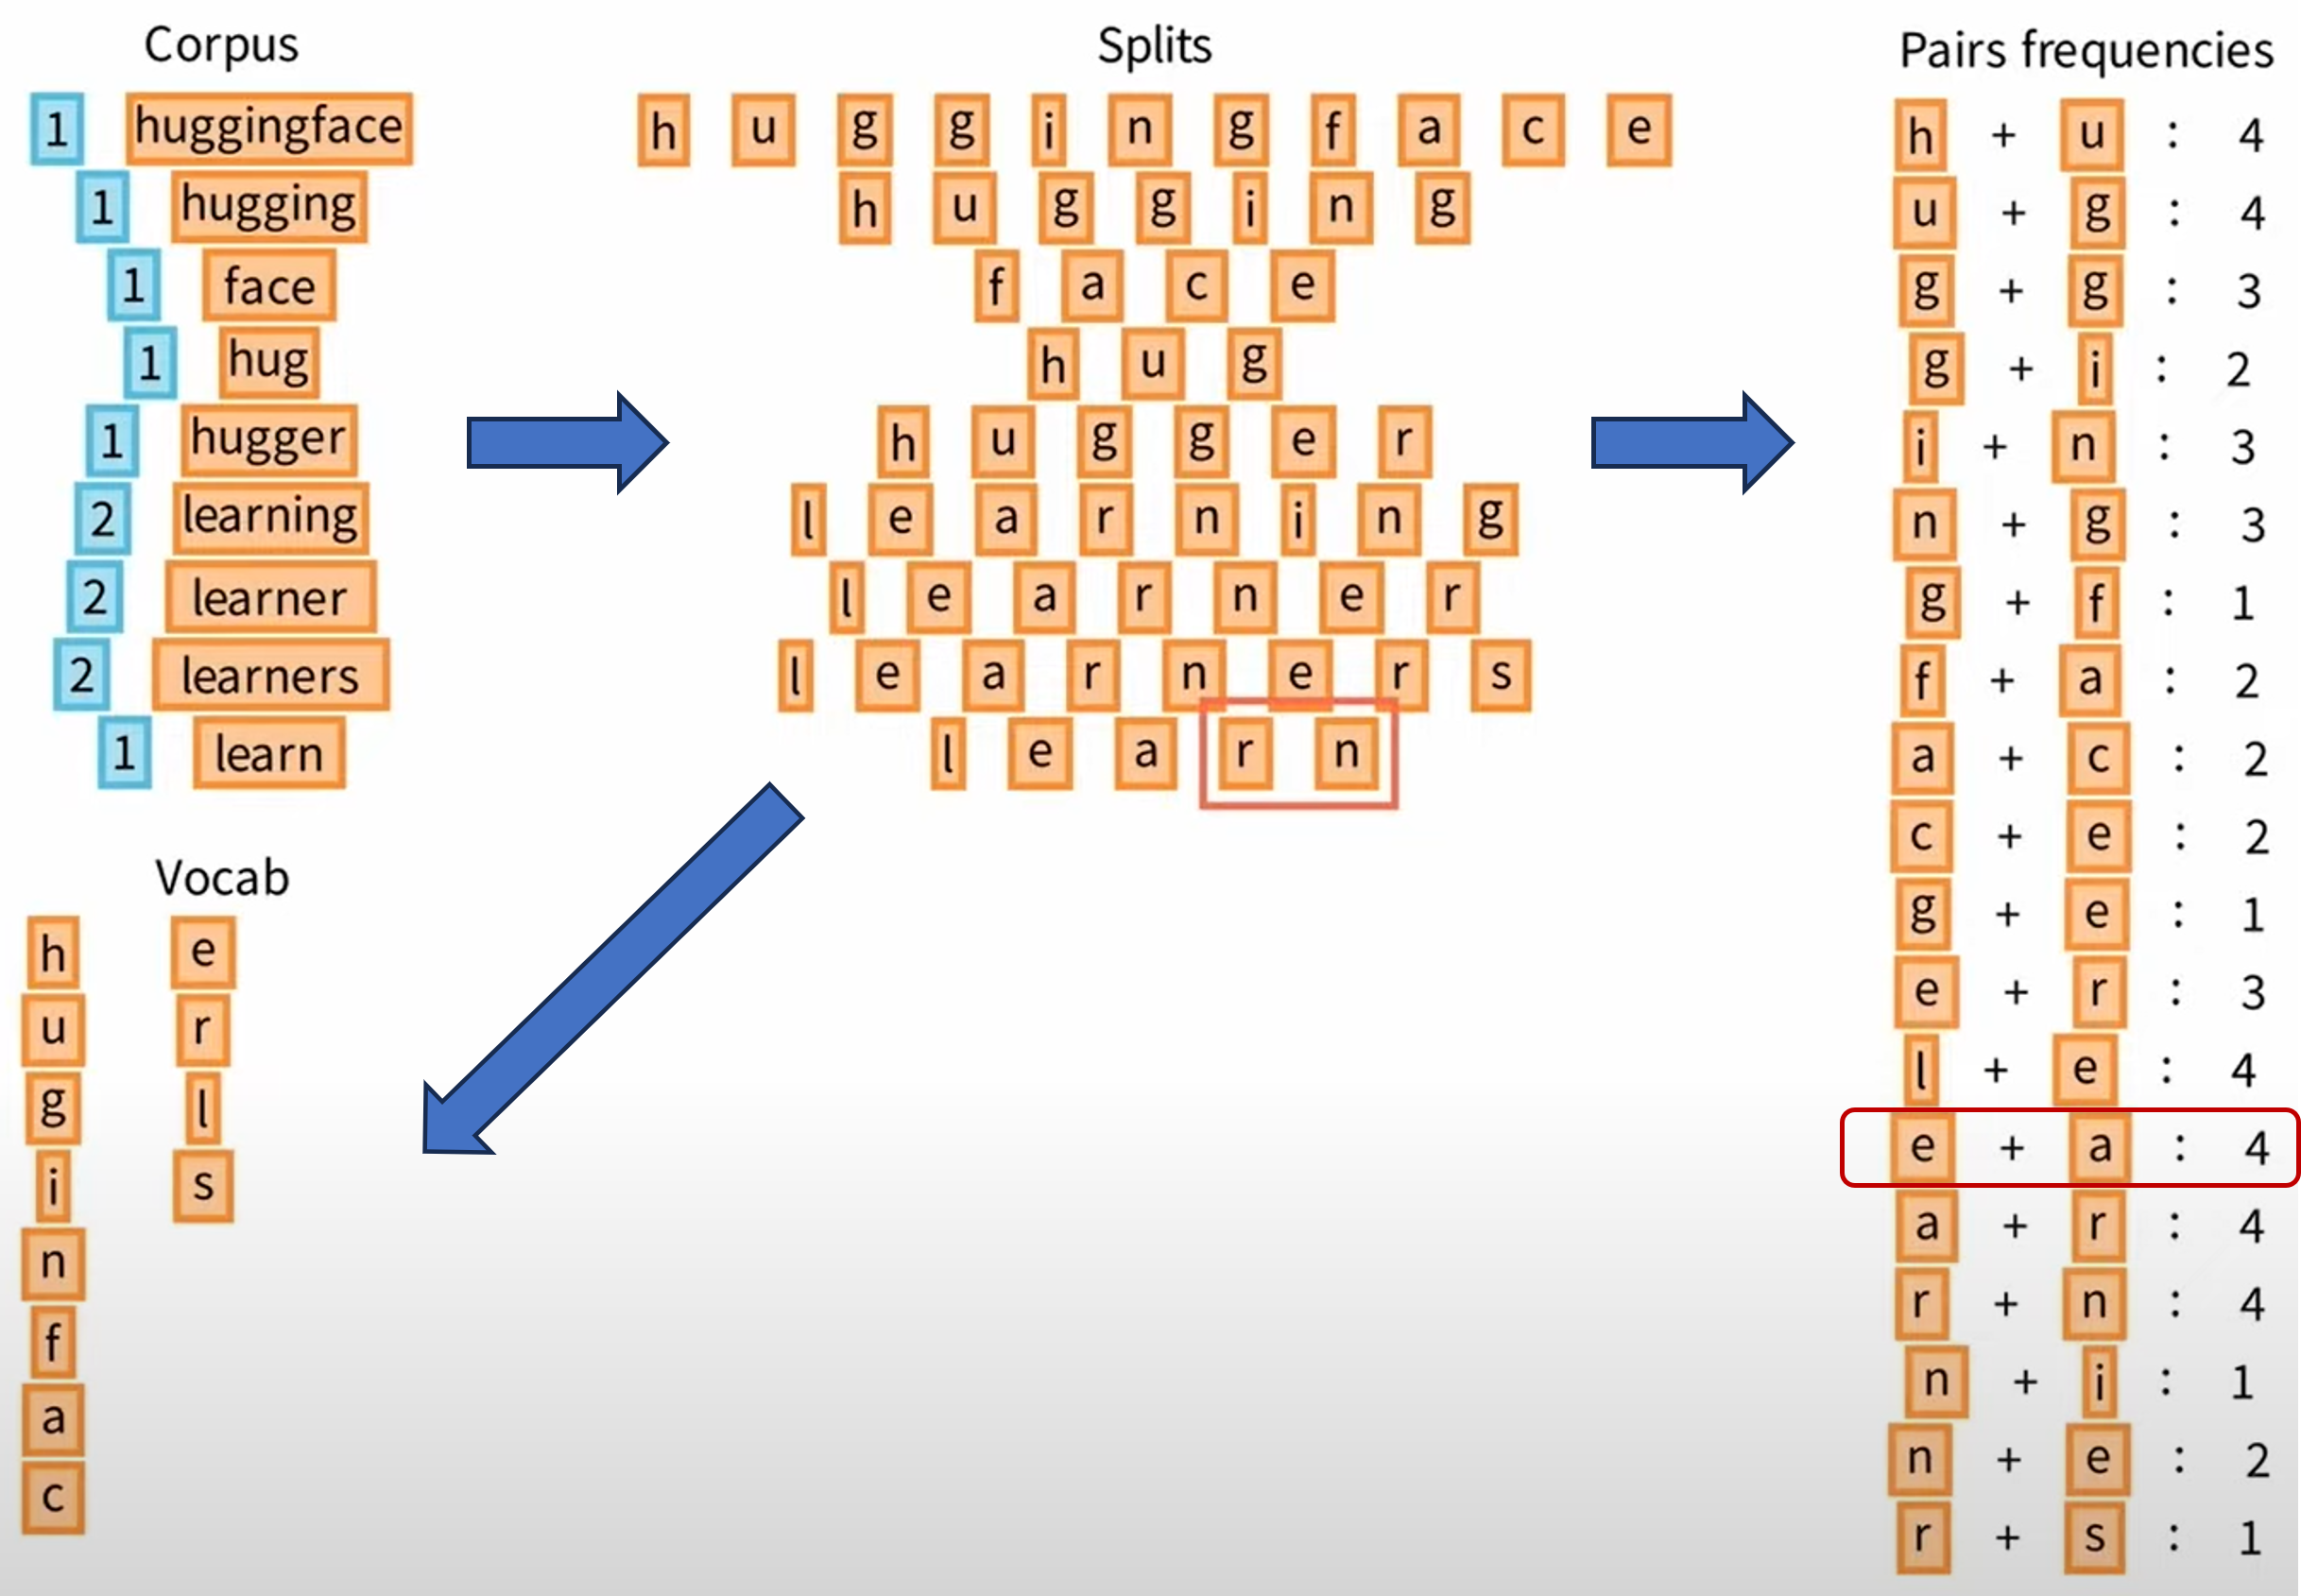
\includegraphics[width=0.45\textwidth]{\toplevelprefix/chapters/chapter7/figs/BPE1.png}\hspace{0.6in} 
    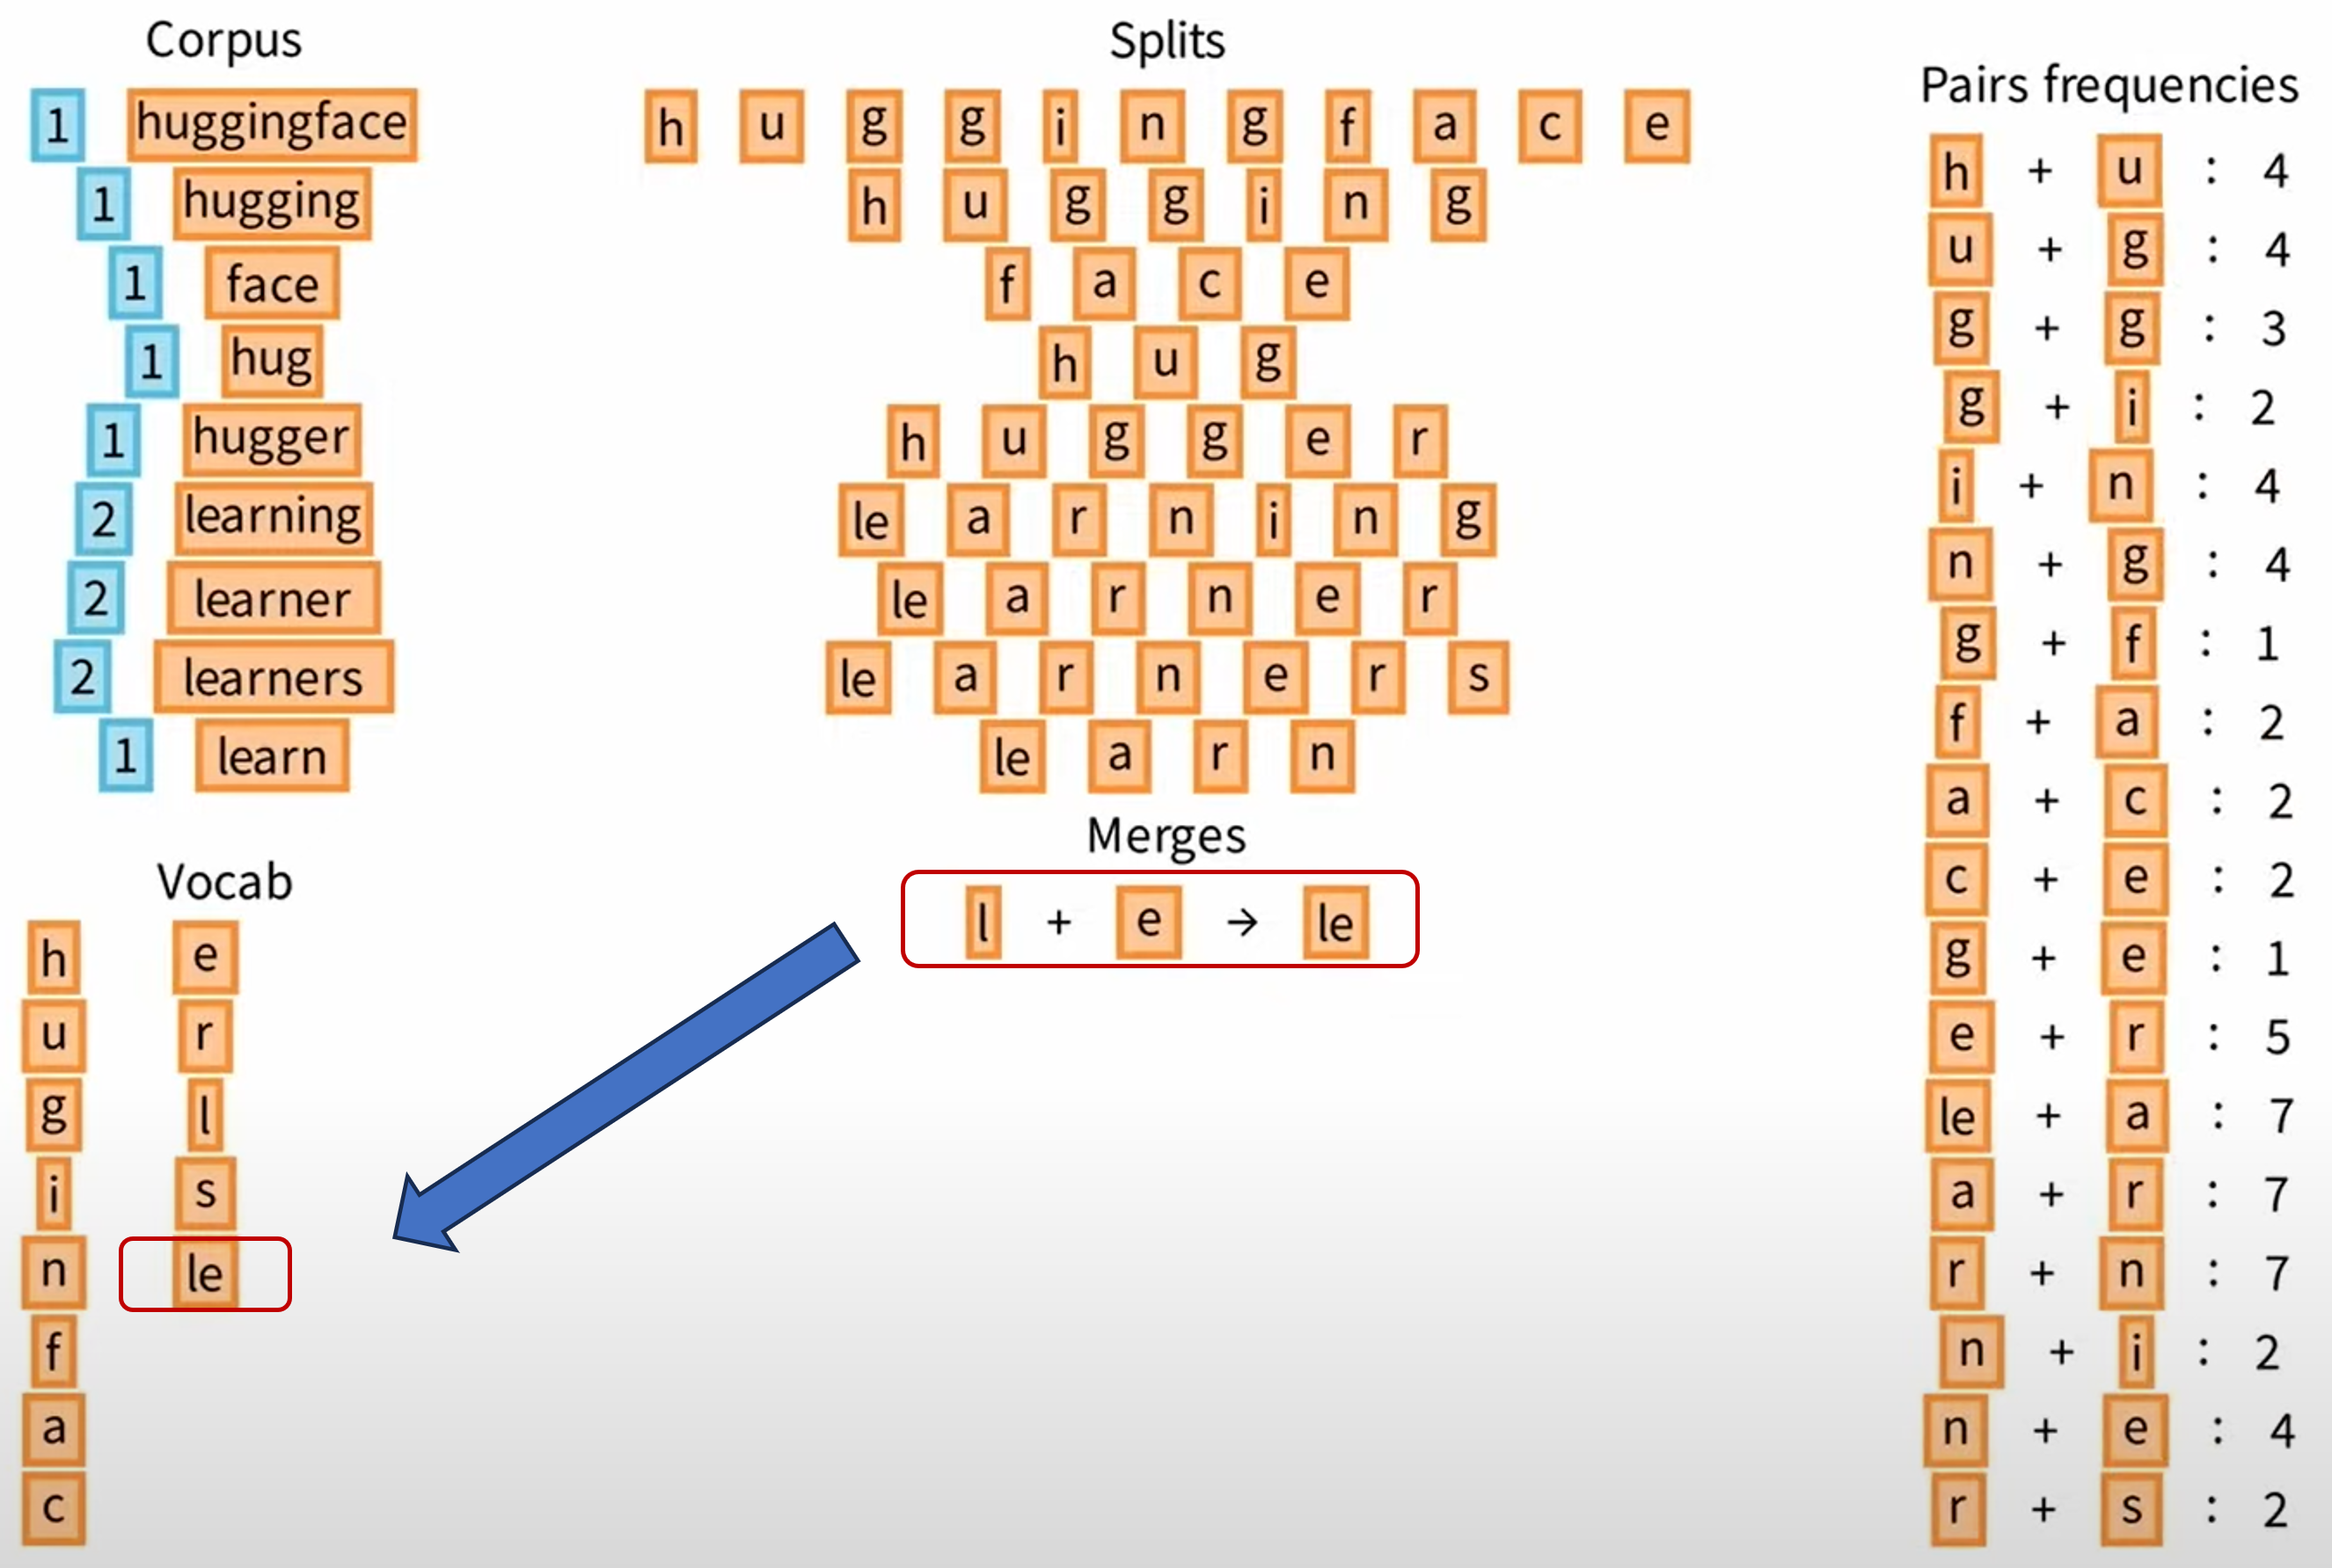
\includegraphics[width=0.45\textwidth]{\toplevelprefix/chapters/chapter7/figs/BPE2.png} 
    \caption{\small {\bf The process of tokenizing text data using BPE.} (Image credit to \url{https://huggingface.co/learn/nlp-course/chapter6/5}). (Left) We begin by analyzing the given text corpus and constructing an initial vocabulary that consists of individual characters (or bytes in the case of byte-level BPE). Then, we compute the frequencies of adjacent character pairs in the corpus. This involves scanning the entire text and counting how often each two-character sequence (bigram) appears. (Right) After computing the frequencies of adjacent character pairs, we identify the most frequent pair in the corpus. This pair is then merged into a new subword unit, which is added to the vocabulary as a single token. This process is repeated iteratively until the predefined vocabulary size is reached. }
    \label{fig:BPE}
\end{figure}
After such a vocabulary is built, a tokenizer can break down a document into tokens (i.e., ``tokenize'' it). BPE uses a similar procedure to tokenize data as in training:
\begin{itemize}
    \item Separate the document into a long list of one-character-long tokens. That is, if the document is ``Hello'' then the initial list is `H', `e', `l', `l', `o'. 
    \item While any two adjacent tokens can be concatenated and their concatenation is another token, we do it, i.e., we replace this pair of tokens with the merged token. Namely, if `He' is a token in the vocabulary, `H', `e', `l', `l', `o' would become `He', `l', `l', `o'.
    \item Repeat the above process until no more merges can be done. At this point, the document is partitioned into the final list (sequence) of tokens.
\end{itemize}

There are many practical and efficiency-based considerations to take into account during tokenization. The above algorithm, as presented, is \textit{very far from optimal} if naively implemented, for instance. We do not cover this topic in great detail; there are many resources online to learn more, such as \href{https://huggingface.co/learn/nlp-course/en/chapter6/5}{HuggingFace tutorials}.

For instance, each token has a corresponding \textit{index} which is just its index in the vocabulary (which after all is just a list of length \(V\)). Thus, the output of most tokenizers is a list of indices, say an element of \([V]^{*}\). Keep in mind that they correspond to substrings of the original document, as shown above.

Once a tokenizer is learned, it can be used as a black box by any language model. For instance, many models have the same (OpenAI-based) tokenizer based on the \texttt{tiktoken} library. In the remainder of this section, we will use such a fixed and pre-built tokenizer for everything, and thus identify each text document \(\vX \in \cT\) with its tokenized version in \([V]^{*}\). Therefore, we may as well consider the text space \(\cT\) as \textit{equal} to the space of token sequences \([V]^{*}\) (and lose nothing essential).

\subsubsection{Training a Language Model}

Once we have each document as a sequence of tokens \(\vX \in [V]^{N} \subseteq [V]^{*} = \cT\), we wish to perform next-token prediction. That is, given a \textit{context} \(\vX_{:n} \in [V]^{n}\) (i.e., the first \(n\) tokens \(\vx_{1}, \dots, \vx_{n} \in [V]\) in the document)\footnote{Note the incongruity with Python notation: here the notation \textit{includes} index \(n\).}, we wish to predict the token \(\vx_{n + 1} \in [V]\) at position \(n + 1\). To do this, we compute the aggregate feature of \(\vX_{:n}\) via \(\vz_{\theta}(\vX_{:n}) \doteq (f_{\theta}^{\ext} \circ f_{\theta})(\vX_{:n}) \in \R^{d}\), and use a classification head \(h_{\theta} \colon \R^{d} \to \Delta_{V}\) (implemented as either a linear layer, MLP, or something slightly more complicated) to project this feature into the \(V\)-dimensional probability simplex \(\Delta_{V}\). This projection \(\vp_{\theta}(\vX_{:n}) \doteq h_{\theta}(\vz_{\theta}(\vX_{:n}))\) serves as an estimated probability distribution of the next token. Then, using the notation \(\vone(\vx_{n + 1}) \in \Delta_{V}\) to be \(1\) in the \(\vx_{n + 1}\)th component and \(0\) elsewhere, the causal language modeling loss is
\begin{equation}\label{eq:clm_loss}
    \min_{\theta}\bc{\cL_{\mathrm{CLM}}(\theta) \doteq \Ex_{\vX}\rs{\frac{1}{N - 1}\sum_{n = 1}^{N - 1}\CE(\vone(\vx_{n + 1}), \vp_{\theta}(\vX_{:n}))}}
\end{equation}
Note how similar this is to a classification loss (say for images); one uses the cross-entropy and tries to align a predicted probability vector with the ground truth. The major difference between these two losses is that in this one, we compute the loss on a whole sequence, where each prediction is correlated with the others (unlike in the i.i.d.~classification case). 

Optimizing this loss is usually called ``pre-training'' in the language model community (contrast with ``post-training'' and, more recently, ``mid-training'', which are methodologies to modify a next-token-predictor for useful tasks).

\textit{Side note:} Why does the first term of \eqref{eq:clm_loss} predict \(\vone(\vx_{2})\), and there is no term which measures the loss to predict the first token? It's because if we wanted to predict the first token, we would have the \textit{empty sequence} as context, and therefore make this first token prediction using a qualitatively different mechanism than that which applies to the other tokens. So actually this model is not trained to predict the \textit{very first} token of any document. The reason this is OK is due to an implementation detail of the tokenizer: often, after building the tokenizer, we insert a \textit{special} token into its vocabulary, called the \textit{beginning-of-string (or document)} token and labeled \texttt{<|bos|>}.\footnote{There are usually several special tokens for different purposes. Existing text containing the special tokens are specially processed.} Then, while processing each document, we add the \texttt{<|bos|>} token at the beginning of the document's token sequence, increasing the length of the tokenized sequence by \(1\). Thus the above causal language modeling objective has a term which involves trying to predict the first token of the document given only the \texttt{<|bos|>} token as context, and so it is a conceptually correct loss.

\subsection{Architecture: Causal CRATE}

For the architecture, we use a standard GPT-2-style transformer, substituting CRATE layers for the transformer layers.\footnote{In direct contravention of the conventions in this book and those of many other communities, the NLP community calls such GPT-2-style transformers (encompassing nearly all current LLMs) ``decoder-only'' transformers. ``Encoder-only'' transformers have a different architecture, and ``encoder-decoder'' transformers concatenate an ``encoder-only'' transformer with a ``decoder-only'' transformer. This despite the fact that ``decoder-only'' transformers \textit{also} compute an encoding of the data!} For completeness, we specify the architecture here.

\paragraph{Embedding.} We first embed the token sequence \(\vX \in [V]^{N}\) to Euclidean space. This is often done by associating each index in \([V]\) with a vector in \(\R^{d}\) using a \textit{massive}\footnote{By ``massive'' we mean that such a structure is often a large fraction of the language model's total size.} array \(\vE \in \R^{V \times d}\), and directly forming the sequence \([\vE_{\vx_{1}}, \dots, \vE_{\vx_{N}}] \in \R^{d \times N}\). The full embedding map \(f_{\theta}^{\emb}\) also applies a positional encoding \(\vE^{\pos} \in \R^{d  \times N_{\max}}\) where \(N_{\max}\) is the maximum number of tokens which are possible to process,\footnote{Modern positional encoding methods have since taken care of this issue and allowed for (in theory) infinite extrapolation, but such methods are more complex to develop, and for simplicity we only introduce the absolute additive positional encoding here.} which yields the embedding map 
\begin{equation}
    f_{\theta}^{\emb}(\vX) \doteq [\vE_{\vx_{1}}, \dots, \vE_{\vx_{N}}] + \vE_{:N}^{\pos}
\end{equation}
The parameters \(\vE\) and \(\vE^{\pos}\) are directly trainable. Since \(\vE\) is so large (and the gradient update is very sparse w.r.t.~it since only a small fraction of the vocabulary is used in each sample), specialized software is used to make sure the memory updates are not too onerous. Notice also that we do not use a class token like in the other sections; more on this later.

\paragraph{Backbone.} We process the embeddings using a CRATE-like backbone which uses causal masking. To motivate causal masking, consider the causal language modeling loss \(\cL_{\mathrm{CLM}}\) defined in \eqref{eq:clm_loss}. The most naive implementation would require us to compute the forward pass \(N\) times in order to backpropagate once. Obviously this is extremely inefficient, since \(N\) can often be in the thousands. In order to scale training with this loss efficiently, we impose a \textit{causal} constraint, i.e.,
\begin{equation}\label{eq:causal_backbone_def}
    \vZ_{\theta}(\vX_{:n}) = \vZ_{\theta}(\vX)_{:n}
\end{equation}
i.e., the \(n\) columns of the token features \(\vZ_{\theta}(\vX_{:n}) \in \R^{d \times n}\) should be the same as the first \(n\) columns of the token features \(\vZ_{\theta}(\vX) \in \R^{d \times N}\) regardless of the positive values of \(n\) and \(N\) such that \(N \geq n\). In effect, this means we can apply the backbone \textit{once} to the whole sequence and compute \(\vZ_{\theta}(\vX)\), then apply \(f_{\theta}^{\ext}\) to each increasing subset \(\vZ_{\theta}(\vX_{:n}) = \vZ_{\theta}(\vX)_{:n}\) as \(n\) grows to the sequence length \(N\). Then we can use all of those to compute the loss.

So now that we want a causal architecture for the backbone, how can we get it? Since the MLP and layer normalizations inside each transformer layer affect each token individually, the only thing that matters for causality is the attention block (or \(\MSSA\) in the case of CRATE). In order to make \(\MSSA\) causal, we define the \(\mathrm{CausalMSSA}\) block as 
\begin{align}
    &\operatorname{CausalMSSA}_{\theta}^{\ell}(\vZ) \doteq \vU_{\out}^{\ell}\mat{\operatorname{CausalSA}([\vU^{1, \ell}]^{\top}\vZ, [\vU^{1, \ell}]^{\top}\vZ, [\vU^{1, \ell}]^{\top}\vZ) \\ \vdots \\ \operatorname{CausalSA}([\vU^{K, \ell}]^{\top}\vZ, [\vU^{K, \ell}]^{\top}\vZ, [\vU^{1, \ell}]^{\top}\vZ)} + \vb_{\out}^{\ell}\vone_{N}^{\top} \\ 
    \text{where} \quad & \operatorname{CausalSA}(\vQ, \vK, \vV) \doteq \vV\softmax\rp{\frac{\operatorname{CausalMask}(\vK^{\top}\vQ)}{\sqrt{p}}} \\ 
    \text{where} \quad & \operatorname{CausalMask}(\vM)_{ij} = \casework{M_{ij}, & \text{if}\ i \geq j, \\ -\infty, & \text{if}\ i < j}.
\end{align}
Here, practitioners say that the causal mask \textit{allows future tokens \(i\) to attend to past tokens \(j\) but not vice versa}. To see why, let us write out the expression for the \(t\)th column of \(\operatorname{CausalSA}(\vQ, \vK, \vV)\):
\begin{equation}
    \operatorname{CausalSA}(\vQ, \vK, \vV)_{t} = \sum_{i = 1}^{t}\vV_{i}\softmax\rp{[\vK_{:t}]^{\top}\vQ_{t}}_{i}
\end{equation}
(where here the non-colon subscript denotes the column). This expression for the \(t\)th token uses no information about any token beyond index \(t\). Therefore \(\operatorname{CausalSA}\), hence \(\operatorname{CausalMSSA}\), hence the whole causal CRATE backbone is causal in terms of the definition in \eqref{eq:causal_backbone_def}, and we unlock the considerable efficiency gains that we were promised. 

\paragraph{Feature extractor.} We use a post-processing step \(f_{\theta}^{\ext}\) which extracts the \textit{feature vector of the last known token} so as to predict the next token. In theory, this means that each token \(\vZ_{\theta}(\vX)_{n}\) should contain rich information about all tokens that come before or at index \(n\), i.e., \(\vx_{1}, \dots, \vx_{n}\), as all of this information should be available for predicting the next token at index \(n + 1\). In practice, only a few of these tokens are really needed for each prediction task. Anyways, the equation for \(f_{\theta}^{\ext}\) is 
\begin{equation}
    f_{\theta}^{\ext}(\vZ_{\theta}(\vX_{:n})) \doteq (\vZ_{\theta}(\vX))_{n}
\end{equation}
where (again) the non-colon subscript is the column. In this case, as promised, we just directly extract the feature vector of the last token in the sequence.

\paragraph{Task-specific head.} For our classification head \(h_{\theta}\), the GPT-2 architecture uses a simple linear layer and a softmax to get the desired probability vectors:
\begin{equation}
    h_{\theta}(\vz) \doteq \softmax(\vW^{\out}\vz + \vb^{\out}),
\end{equation}
where \(\vW^{\out} \in \R^{V \times d}, \vb^{\out} \in \R^{V}\). Some other more modern architectures use small MLPs and layer normalizations, but the idea is very much the same. Note that this linear layers also have large memory usage (because \(V\) is very large), and form a bottleneck in training; there has been significant effort attempting to circumvent it.

All these architectural choices mean that causal training is extremely efficient relative to non-causal training:
\begin{itemize}
    \item We only need \textit{one forward pass} through the backbone to compute the loss for the whole sequence.
    \item The feature extraction is basically \textit{free}.
    \item All tokens can be pushed through the task-specific head \textit{in parallel}.
\end{itemize}

\subsection{Optimization Strategy}

We train our language model using end-to-end stochastic optimization. One remaining issue is that, in practice, different documents in a batch have different lengths (in terms of the number of tokens required for each sequence), but as of the time of writing this book, the main deep learning frameworks by and large allow only ``rectangular'' tensors, which do not accommodate this behavior. To try to resolve this issue, we just insert a special padding token \texttt{<|pad|>} for all shorter samples in the batch, so that we can batch-process everything using rectangular tensors. At each timestep \(k\), we:
\begin{itemize}
    \item Subsample \(B\) different tokenized documents \(\{\vX_{b}^{(k)}\}_{b = 1}^{B} \subseteq \cT = [V]^{*}\), each with length \(N_{b}^{(k)}\).
    \item Compute \(N_{\max}^{(k)} \doteq \max_{b \in [B]}N_{b}^{(k)}\) and pad each \(\vX_{b}^{(k)}\) to length \(N_{\max}^{(k)}\) using a special padding token.
    \item Compute the features \(\vZ_{\theta}(\vX_{b}^{(k)})\).
    \item Compute the predicted distributions \(\vp_{\theta}(\vX_{b, :n}^{(k)}) \doteq (h_{\theta} \circ f_{\theta}^{\ext})(\vZ_{\theta}(\vX_{b}^{(k)})_{:n})\).
    \item Form the surrogate stochastic loss 
    \begin{equation}
        \hat{\cL}_{\mathrm{CLM}}^{(k)}(\theta) \doteq \frac{1}{B(N_{\max}^{(k)} - 1)}\sum_{b = 1}^{B}\sum_{n = 1}^{N_{\max}^{(k)}-1}\CE(\vone(\vx_{b, n + 1}^{(k)}), \vp_{\theta}(\vX_{b, :n}^{(k)}))).
    \end{equation}
    \item Compute one step of an optimization algorithm on \(\theta\), giving the following iteration:
    \begin{equation}
        \theta^{(k + 1)} \doteq \textsc{OptUpdate}^{(k)}(\theta^{(k)}; \nabla_{\theta}\hat{\cL}_{\mathrm{CLM}}^{(k)}).
    \end{equation}
\end{itemize}

\subsection{Evaluation Methodology} \label{sub:clm_text_evals}

There are several ways to evaluate a trained transformer language model.
\begin{itemize}
    \item On a holdout dataset of arbitrary text, we can evaluate \(\cL_{\mathrm{CLM}}\) on it; lower losses are better since they mean the model's sampling yields better performance.
    \item On a multiple choice question dataset, for each question we can put it as the context and check the estimated probability of the correct answer being generated.
    \item We can also test the \textit{text generation} capabilities. Namely, we can repeatedly sample from the model's probability distribution over the next token given the context. Each time we sample we generate a new token, which we print and add to the context. This allows us to sample from the LLM, and judge the generated samples however we please.\footnote{Having to re-run the model on each token every time can become prohibitively expensive. Clever storages of different internal features of the language model (such as the so-called \textit{\(K\)-\(V\) cache}), along with the causality of the architecture, can dramatically reduce the cost of sampling.}
\end{itemize}
In this section, we perform the first kind of evaluation exclusively.

\subsection{Experimental Setup and Results}

Since our causal CRATE architecture is directly built upon GPT-2, we compare the optimal settings for GPT-2 as given by the NanoGPT repository \citep{nanogpt} with the same settings applied to CRATE for a fair comparison.

\paragraph{Model architecture.} We use the GPT-2 tokenizer, which has vocabulary size \(V = 50257\), including a special token for \texttt{<|pad|>}.\footnote{The \texttt{<|bos|>} token is not included in this setup, although it is very common in modern language models.} The context length is \(N_{\max} = 1024\). The backbone model follows the GPT2-Base architecture \citep{radford2019language} with the appropriate alterations to have causal CRATE layers, and we compare against GPT2-Small and GPT2-Base.

\paragraph{Datasets and optimization.} For training causal CRATE, we follow the implementations in the NanoGPT repository \citep{nanogpt}. Specifically, we use a batch size of 384 and train for 600,000 steps with the Adam optimizer~\citep{kingma2014adam}. For the Adam optimizer, we use $(\beta_1, \beta_2)=(0.9, 0.95)$ and weight decay of $0.1$. For the learning rate schedule, we apply a linear warm-up and cosine decay, with a peak value of $\eta=6\times 10^{-4}$ at the $2,000$th iteration, and minimum value $6\times 10^{-5}$. The training and validation losses over iterations are shown in \Cref{fig:crate-text-evals}. The training/validation loss converges around $3.37$ after training with a batch size of $384$ and $600,000$ iterations. In comparison, the open GPT-2 implementation is pre-trained on OpenWebText with a batch size of $512$ and $600,000$ steps and converges to a validation loss of $2.85$ \citep{nanogpt}.  

\begin{figure}
    \centering
    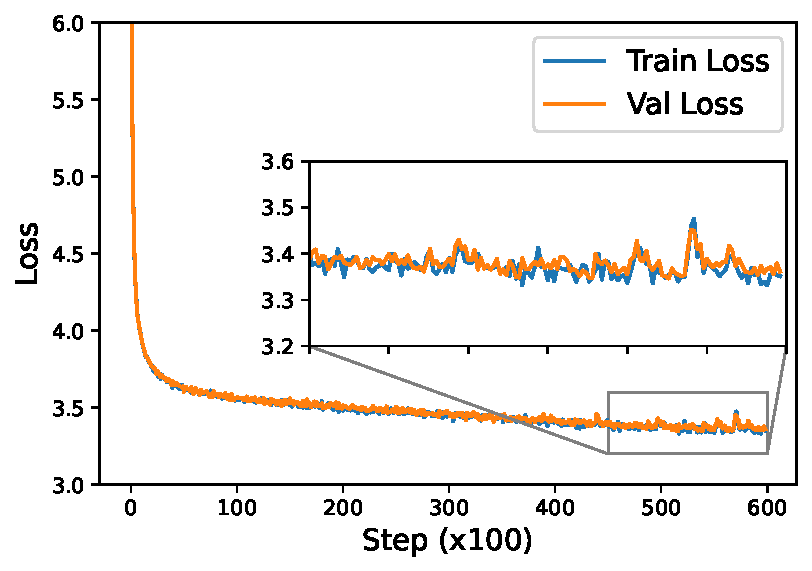
\includegraphics[width=0.5\textwidth]{\toplevelprefix/chapters/chapter7/figs/gpt-loss.pdf}
    \caption{\bf The loss curve of CRATE-GPT-Base trained on the OpenWebText dataset.}
    \label{fig:crate-text-evals}
\end{figure}

\paragraph{Experiment results.}

\Cref{tab:gpt-eval} demonstrates that CRATE models achieve reasonable performance on the causal language modeling loss across a variety of datasets compared to GPT-2 models with similar parameter counts and similar architectures.


\begin{table}
\def\arraystretch{1.1}
    \small
    \caption{\small Zero-shot cross-entropy loss of the CRATE-GPT2-Base model and GPT2-Small, GPT2-Base model evaluated on the test split of the datasets ($\downarrow$ lower is better). 
    }
    \centering
    \begin{tabular}{ccccccc}
    \hline
    & \#parameters & \textbf{OWT} & \textbf{LAMBADA} & \textbf{WikiText} & \textbf{PTB} & \textbf{Avg} \\
     \hline
     GPT2-Base  & {124M} & 2.85$\downarrow$ & 4.12$\downarrow$ & 3.89$\downarrow$ & 4.63$\downarrow$ & 3.87$\downarrow$ \\
     {GPT2-Small } &  {64M} & {3.04} & {4.49} & {4.31} & {5.15} & {4.25} \\
     Causal-CRATE-Base & {60M} & 3.37 & 4.91 & 4.61 & 5.53 & 4.61 \\
     \hline
    \end{tabular}
    \label{tab:gpt-eval}
\end{table} 































\section{Scaling White-Box Transformers}\label{sec:scalable}

In this section, we will discuss three ways in which various parts of CRATE-type models can be scaled up or made more efficient while still remaining white-box. These developments mix both conceptual and empirical insights, and can be viewed as case studies about how to use white-box understanding to improve deep learning models in practice. The tasks that we use to evaluate the methods will be image classification and next-token-prediction, the data will be ImageNet and OpenWebText respectively, the optimization procedure will be the same backpropagation, and the only thing that changes is the architecture.

\subsection{Increasing Network Width: CRATE-\texorpdfstring{\(\alpha\)}{alpha}}\label{sub:crate_alpha_experiments}

\begin{figure}[t]
    \centering 
    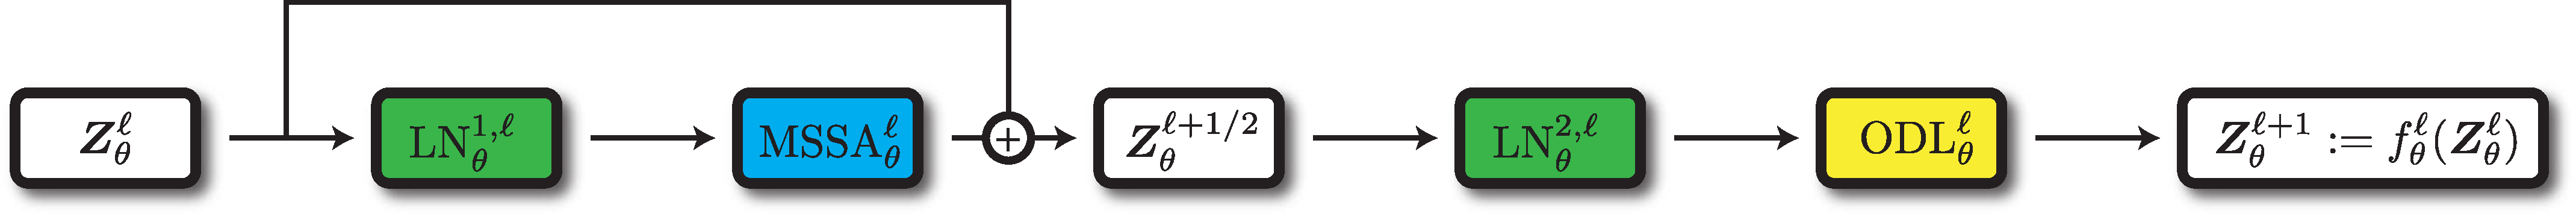
\includegraphics[width=\textwidth]{\toplevelprefix/chapters/chapter7/figs/crate_alpha_backbone.pdf}
    \caption{\small\textbf{One layer of the CRATE-\(\alpha\) backbone.} The difference from CRATE is that the \(\ISTA_{\theta}^{\ell}\) block is replaced by the \(\operatorname{ODL}_{\theta}^{\ell}\) block, which performs several \(\ISTA\) steps with an overcomplete dictionary.}
    \label{fig:crate_alpha_backbone}
\end{figure}


One design decision enforced by the CRATE framework is the \textit{width} of the nonlinearity in the network. In a regular transformer, the width is usually set to \(4\), \(8\), or \(\frac{11}{3}\) times the feature dimension. However, CRATE enforces that the width is exactly equal to the feature dimension, i.e., the dictionaries \(\vD^{\ell}\) are square, which could lead to reduced performance. The fundamental reason that the CRATE framework constrains us to this choice is as follows:
\begin{itemize}
    \item The ISTA block takes a \textit{single} step of optimization for dictionary learning.
    \item Usually one step of any iterative optimization algorithm cannot effectively optimize the objective. So then why does this work?
    \item Optimization algorithms usually converge very quickly if and only if they have good initializations, or \textit{warm starts}. The ISTA block has a warm start --- it treats the input features as an initialization to the resulting sparse codes.
    \item This enforces that the input features and sparse codes have the same dimension. Namely, ISTA learns a complete sparsifying dictionary (cf \Cref{ch:classic}).
\end{itemize}
Thus if we want to use a wide dictionary, we need ISTA to perform \textit{overcomplete} dictionary learning. This means we cannot have the same warm start (as our sparse codes have a larger dimension than our features), and need more iterations to converge to a sparse code. Hence the step from features \(\vZ_{\theta}^{\ell + 1/2}\) to sparse codes \(\vZ_{\theta}^{\ell + 1}\) would no longer be 
\begin{equation}
    \vZ_{\theta}^{\ell + 1} = \ISTA_{\theta}^{\ell}(\vZ_{\theta}^{\ell + 1/2} \mid \vZ_{\theta}^{\ell + 1/2})
\end{equation}
where the \(\ISTA_{\theta}^{\ell}\) function is defined as (by an abuse of notation from earlier sections)
\begin{equation}
    \ISTA_{\theta}^{\ell}(\vZ \mid \vY) \doteq \ReLU(\vZ - \beta (\vD^{\ell})^{\top}(\vD^{\ell}\vZ - \vY) + \beta \lambda \vone_{s}\vone_{n}^{\top})
\end{equation}
but rather the following iteration:
\begin{equation}
    \vZ_{\theta}^{\ell + 1} = \vA_{\theta}^{\ell, T}; \qquad \vA_{\theta}^{\ell, t + 1} = \ISTA_{\theta}^{\ell}(\vA_{\theta}^{\ell, t} \mid \vZ_{\theta}^{\ell + 1/2}) \quad \forall 0 \leq t < T; \qquad \vA_{\theta}^{\ell, 0} = \vzero_{s \times n},
\end{equation}
i.e., running proximal gradient on the LASSO objective for \(T \geq 1\) steps in the forward pass at each layer, initialized at \(\vzero_{s \times n}\). In this circumstance, the dictionary can be as wide as needed, i.e., \(\vD^{\ell} \in \R^{s \times d}\) where \(s \geq d\) (usually one takes \(s = 4d\) in practice). 

\begin{table}[b]
    \centering
    \begin{tabular}{@{}lcccccccc@{}}
    \toprule
     &  & \multicolumn{3}{c}{Detection} &  \multicolumn{3}{c}{Segmentation} \\ 
    Model & AP$_{50} \uparrow $ & AP$_{75} \uparrow $ & AP $\uparrow$ & AP$_{50} \uparrow$ & AP$_{75} \uparrow $ & AP $\uparrow$ \\ 
    \midrule
    \midrule
    CRATE-\(\alpha\)-B/8 & 3.5 & 1.1 & 1.5 & 2.2 & 1.0 & 1.1 \\
    CRATE-\(\alpha\)-L/8 & \textbf{4.0} & \textbf{1.7} & \textbf{2.0} & \textbf{2.7} & \textbf{1.1} & \textbf{1.4} \\
    \midrule
    \color{gray}CRATE-B/8 & \color{gray}2.9 & \color{gray}1.0 & \color{gray}1.3 & \color{gray}2.2 & \color{gray}0.7 & \color{gray}1.0 \\
    \color{gray}ViT-B/8 & \color{gray}0.8 & \color{gray}0.2 & \color{gray}0.4 & \color{gray}0.7 & \color{gray}0.5 & \color{gray}0.4 \\
    \bottomrule
    \end{tabular}
    \caption{\small \textbf{Object detection and fine-grained segmentation via MaskCut on COCO val2017~\citep{lin2014microsoft}}. Here all models are trained with patch size \(8\) instead of \(16\). Compared with existing models such as CRATE and ViT, the CRATE-\(\alpha\) model family noticeably has improved performance as well as scalability.}
    \label{tab:crate_alpha_detection_segmentation}
\end{table}

However, this presents an empirical problem. Using the above configuration, if \(\vZ^{\ell + 1/2} \in \R^{d \times n}\), then \(\vZ^{\ell + 1} \in \R^{s \times n}\), which can have an arbitrarily large feature dimension. In practice, we want the feature dimension at each layer to be the same. So this sets up a practical trichotomy for designing the network, namely, we \textit{cannot} have \textit{all} of the following desiderata:
\begin{enumerate}
    \item The feature dimension at each layer is the same.
    \item The dictionary is wide, i.e., overcomplete.
    \item The output of the nonlinearity is the sparse codes of the input with respect to the dictionary.
\end{enumerate}
In practice, giving up (1) is less tractable for efficiency reasons. Giving up (2) leads to the usual CRATE framework. Giving up (3) leads to a wide version of CRATE, i.e., CRATE-\(\alpha\), which has the following nonlinearity to get from \(\vZ^{\ell + 1/2}\) to \(\vZ^{\ell + 1}\):
\begin{equation}
    \vZ_{\theta}^{\ell + 1} = \vD^{\ell}\vA_{\theta}^{\ell, T}; \qquad \vA_{\theta}^{\ell, t + 1} = \ISTA_{\theta}^{\ell}(\vA_{\theta}^{\ell, t} \mid \vZ_{\theta}^{\ell + 1/2}); \qquad \vA_{\theta}^{\ell, 0} = \vzero,
\end{equation}
i.e., it takes the sparse codes obtained via proximal gradient descent and multiplies by the dictionary to get the denoised version of the input. Thus CRATE-\(\alpha\)'s nonlinearity computes a denoised version of the input which is amenable to sparse coding, not the actual sparse codes themselves. The map from \(\vZ_{\theta}^{\ell + 1/2}\) to \(\vZ_{\theta}^{\ell + 1}\) here is called the Overcomplete Dictionary Learning (ODL) block and denoted \(\operatorname{ODL}_{\theta}^{\ell}\), i.e.,
\begin{equation}
    \vZ_{\theta}^{\ell + 1}(\vX) \doteq \operatorname{ODL}_{\theta}^{\ell}(\vZ_{\theta}^{\ell + 1/2}(\vX)).
\end{equation}



\begin{figure}[t]
    \centering 
    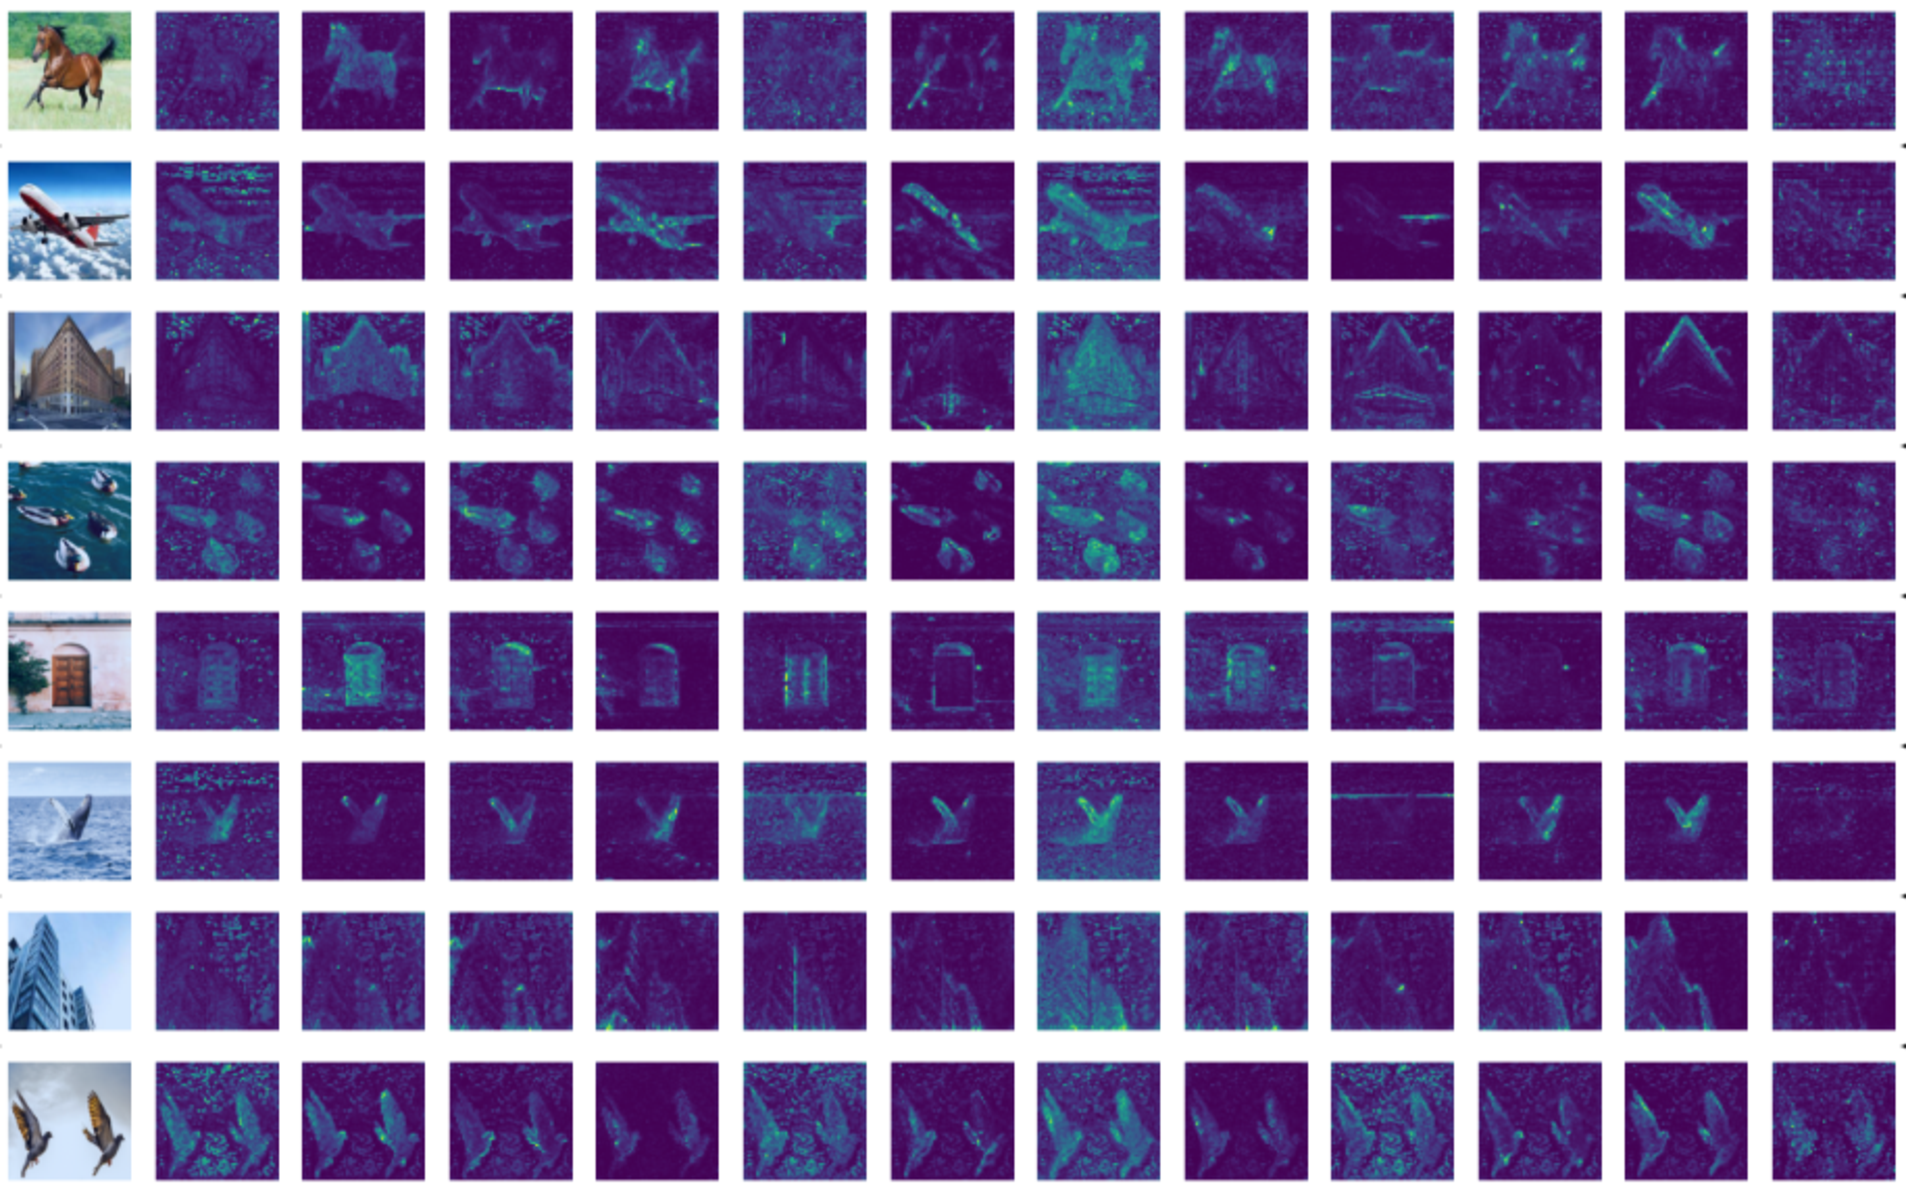
\includegraphics[width=\textwidth]{\toplevelprefix/chapters/chapter7/figs/crate_alpha_semantic_heads.pdf}
    \caption{\small\textbf{Saliency maps from CRATE-\(\alpha\) with patch size \(8\).} Each row is a different image and each column corresponds to a different attention head in the last layer. We observe that the saliency maps strongly correspond to the objects in the input image.}
    \label{fig:crate_alpha_saliency_maps}
\end{figure}



\begin{table}
    \centering 
    \begin{tabular}{@{}lcccc@{}}
    \toprule
    Model & GPT-2-B(ase) & CRATE-B & CRATE-\(\alpha\)-S(mall) & CRATE-\(\alpha\)-B \\ 
    \midrule
    \midrule
    \# parameters & 124M & 60M & 57M & 120M \\
    OWT val.~loss & 2.85 & 3.37 & 3.28 & 3.14 \\
    \bottomrule
    \end{tabular}
    \caption{\small\textbf{Validation loss in language modeling.} Here all models are pre-trained on most of OpenWebText, and the validation cross-entropy loss is measured on a hold-out subset of OpenWebText. CRATE-\(\alpha\) shows significant improvement over the CRATE design, though there still exists a gap with traditional transformers like GPT-2.}
    \label{tab:crate_alpha_lm}
\end{table}

The CRATE-\(\alpha\) layer is shown in \Cref{fig:crate_alpha_backbone}. In practice this modification of CRATE performs very well at larger scales. For example, when we pre-train CRATE-\(\alpha\) models on ImageNet-21K, unsupervised tasks like segmentation (see \Cref{fig:crate_alpha_saliency_maps} and \Cref{tab:crate_alpha_detection_segmentation}) generally have significantly improved performance compared to CRATE. Similar trends are present in language model training using causal self-attention (see \Cref{tab:crate_alpha_lm}). Overall, it is a promising avenue to scaling up the performance to match black-box models such as transformers.\footnote{Note that the experimental results in this section use a slightly different model architecture, which add very slight empirical gains. The changes are: (1) an additional residual connection on the ODL block, (2) modifying \(\ISTA\) to use two separate dictionaries instead of \(\vD^{\ell}\) and \((\vD^{\ell})^{\top}\).} 


\subsection{Linear Time Complexity Transformers}\label{sub:tost_experiments}

In practice, deep learning models suffer from bottlenecks in space and time complexity, representing problem sizes beyond which they cannot scale given fixed resources. One such bottleneck, particularly meaningful when dealing with data where each sample is itself high-dimensional and rich (such as long streams of text or videos), is the \textit{time complexity} of processing long sequences of data. In order to alleviate the time complexity of processing data using transformers, in \Cref{sub:tost} we proposed a \textit{token statistics self-attention} operator \(\TSSA_{\theta}^{\ell}\). We now build a \textit{token statistics transformer}, called ToST, around it, which we can use for long-context tasks. In particular, we can use the following layer (depicted in \Cref{fig:tost_backbone}) as a drop-in replacement for a backbone layer in CRATE:
\begin{align}
    \vZ_{\theta}^{\ell + 1/2}(\vX)
    &= \vZ_{\theta}^{\ell}(\vX) + \TSSA_{\theta}^{\ell}(\LN_{\theta}^{1, \ell}(\vZ_{\theta}^{\ell}(\vX))) \\ 
    \vZ_{\theta}^{\ell + 1}(\vX)
    &= \vZ_{\theta}^{\ell + 1/2}(\vX) + \MLP_{\theta}^{\ell}(\LN_{\theta}^{2, \ell}(\vZ_{\theta}^{\ell + 1/2}(\vX)))
\end{align}
where the \(\TSSA\) block is defined as in \Cref{sub:tost}. Notice that this is exactly the same as the vision transformer architecture discussed in \Cref{sub:contrastive_learning_architecture}, except that \(\TSSA\) replaces the conventional multi-head self-attention block \(\MHSA\). Regardless, the computational complexity of the forward pass of this layer is linear in all problem variables --- sequence length, feature dimension, number of heads, and head dimension.

\begin{figure}[!htbp]
    \centering 
    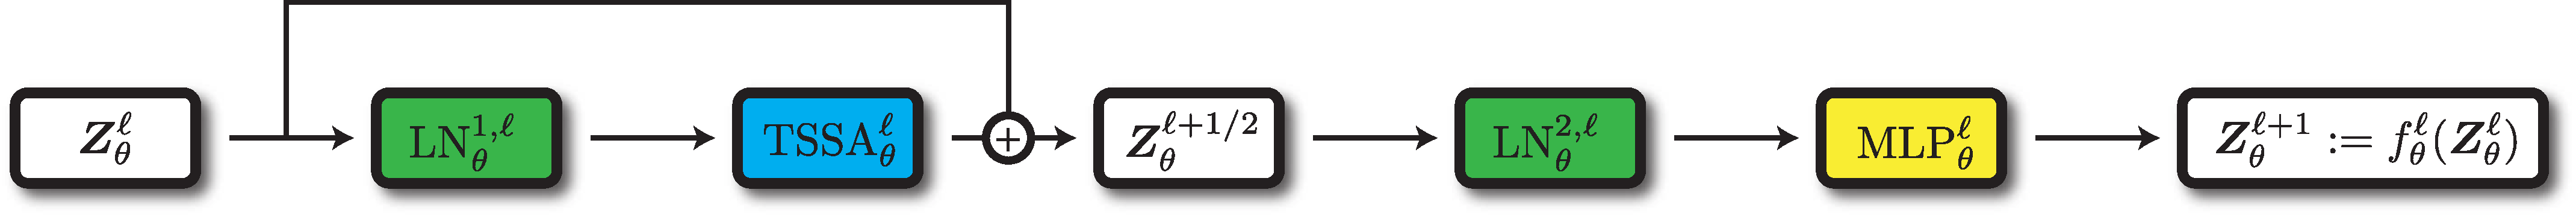
\includegraphics[width=\textwidth]{\toplevelprefix/chapters/chapter7/figs/tost_backbone.pdf}
    \caption{\small\textbf{One layer of the ToST backbone}. Token representations go through layer-norms, the token statistics self-attention (TSSA) operator, and an MLP, in order to form the layer's output.}
    \label{fig:tost_backbone}
\end{figure}

\begin{table}[t]
    \centering 
    \resizebox{\textwidth}{!}{
    \begin{tabular}{@{}lccc|cc|cc@{}}
    \toprule
    Datasets & ToST-T(iny) & ToST-S(mall) & ToST-M(edium) &  { \color{gray} XCiT-S} &  { \color{gray}XCiT-M} &  {\color{gray}ViT-S} & {\color{gray}ViT-B(ase)}\\ 
    \toprule
     \# parameters & 5.8M & 22.6M & 68.1M &  { \color{gray}24.9M }& { \color{gray}80.2M } & { \color{gray} 22.1M } & { \color{gray}86.6 M } \\
    \midrule
     ImageNet & 67.3 & 77.9 & 80.3 &  { \color{gray} 80.5} & { \color{gray} 81.5 } & { \color{gray} 79.8} & { \color{gray} 81.8} \\
     ImageNet ReaL & 72.2  & 84.1 & 85.6 &  { \color{gray} 85.6 } & { \color{gray} 85.9} & { \color{gray} 85.6 } & { \color{gray} 86.7 }\\
     \midrule
     CIFAR10 & 95.5 & 96.5 & 97.5 &  { \color{gray} 98.1} & { \color{gray} 98.3} & { \color{gray} 98.6} & { \color{gray} 98.8}\\
     CIFAR100 & 78.3 & 82.7 & 84.5 &  { \color{gray} 86.1} & { \color{gray} 87.6} & { \color{gray} 88.8} & { \color{gray} 89.3}\\
     Oxford Flowers-102 & 88.6 & 92.8 & 94.2 &  { \color{gray} 93.9} & { \color{gray} 94.0} & { \color{gray} 94.0}& { \color{gray} 95.7}\\
     Oxford-IIIT-Pets & 85.6 & 91.1 & 92.8 &  { \color{gray} 92.9} & { \color{gray} 94.0} & { \color{gray} 92.8} & { \color{gray} 94.1} \\
     \bottomrule
    \end{tabular}%
    }
    \caption{\small \textbf{Linear probing classification accuracy of ToST} on various datasets with different model sizes when the backbone is pre-trained for ImageNet-1K classification. We observe that, compared to the XCiT (a empirically-designed transformer-like architecture specialized for efficient processing of long sequences) and the ViT, ToST maintains relatively similar performance, even while enjoying benefits like faster runtime and white-box design.}
    \label{tab:tost_linear_probing}
\end{table}

\begin{table}[!htbp]
    \centering 
    \begin{tabular}{@{}lcccccc@{}}
        \toprule
        Model & \# params & OWT & Lambada & Wikitext & PTB & Avg $\downarrow$ \\ \midrule
        GPT-2-Base & 124M & 2.84 & 4.32 & 4.13 & 5.75 & 4.26 \\
        ToST-Base & 110M & 3.20 & 4.98 & 4.77 & 6.39 & 4.84 \\
        ToST-Medium & 304M & 2.88 & 4.45 & 4.30 & 5.64 & 4.32 \\
        ToST-Large & 655M & 2.72 & 4.32 & 3.99 & 5.03 & 4.02 \\ \bottomrule
    \end{tabular}%
    \caption{\small\textbf{Language modeling validation loss} computed on (holdout sets of) a variety of natural language datasets, after pre-training the model on that dataset. We observe that ToST scales well, so that ToST-Large surpasses the baseline GPT-2-Base in causal language modeling, while enjoying superior efficiency in long contexts.}
    \label{tab:tost_lm}
\end{table}

\begin{table}
    \centering
    
    \begin{tabular}{@{}lccccccc@{}}
            \toprule
            Model        & ListOps  & Text     & Retrieval & Image    & Pathfinder & Avg      \\
            \midrule
            \midrule
            Reformer              & \textbf{37.27} & 56.10             & 53.40              & 38.07             & 68.50               & 50.56             \\
            BigBird               & 36.05             & 64.02             & 59.29              & 40.83             & 74.87                & 54.17             \\
            LinFormer         & 16.13             & \underline{65.90} & 53.09              & 42.34             & \underline{75.30}               & 50.46             \\
            Performer             & 18.01             & 65.40             & 53.82              & 42.77             & \textbf{77.05}                & 51.18             \\
            Transformer           & 37.11             & 65.21             & \underline{79.14}              & \underline{42.94}             & 71.83              & \underline{59.24}            \\
            ToST & \underline{37.25}    & \textbf{66.75}    & \textbf{79.46}     & \textbf{46.62}    &    69.41      &     \textbf{59.90}\\
            
            \bottomrule
        \end{tabular}%
    \caption{\small \textbf{Long-Range Arena (LRA) performance comparison of ToST(-B) versus the top transformer variants optimized for long-context.} Long-Range Arena is a family of benchmarks that test the long sequence modeling capability of algorithms and architectures, by fixing the dataset and evaluation mechanism. ToST scores at the top of the leaderboard compared to all known transformer variants, including XCiT and the regular (ViT) transformer (cf \Cref{tab:tost_linear_probing}). Moreover, ToST has the lowest time- and space-complexity inference. (In this table, the best score for a particular benchmark is bolded, and the second-best score is underlined.)}
    \label{tab:tost_lra_results}
\end{table}

Moreover, the proposed architecture, named ToST (for ``Token Statistics Transformer'') performs well at vision tasks (i.e., \Cref{tab:tost_linear_probing}) and language tasks (i.e., \Cref{tab:tost_lm}). This is especially true for long-sequence-length tasks (cf \Cref{tab:tost_lra_results}), where it is both more performant and much more efficient than conventional transformers and all other transformer-like architectures.

\subsection{Attention-Only Transformers} \label{sub:aot_experiments}

Another bottleneck to remove from deep learning models, specifically transformer-like architectures, is the memory bottleneck that comes from massive matrix multiplications in MLPs, where the internal dimension is far greater than the feature dimension \(d\). It thus is an interesting and important question to ask: do we \textit{really} need the MLP inside a transformer, and how good can the performance get without it? To explore this question, we use the attention-only-transformer (AoT) architecture (see \Cref{sub:aot}), depicted in \Cref{fig:aot_backbone}. Namely, each layer is simply of the form 
\begin{equation}
    \vZ_{\theta}^{\ell + 1}(\vX) = \vZ_{\theta}^{\ell}(\vX) + \MSSA_{\theta}^{\ell}(\LN_{\theta}^{\ell}(\vZ_{\theta}^{\ell}(\vX))).
\end{equation}
In our implementation, we also experimented with using multi-head self-attention (MHSA) in place of MSSA. It turns out that this architecture is \textit{also} viable, though the depth of the network needs to be much greater in order to achieve equivalent performance to the usual CRATE or transformer architecture. %

\begin{figure}[!htbp]
    \centering 
    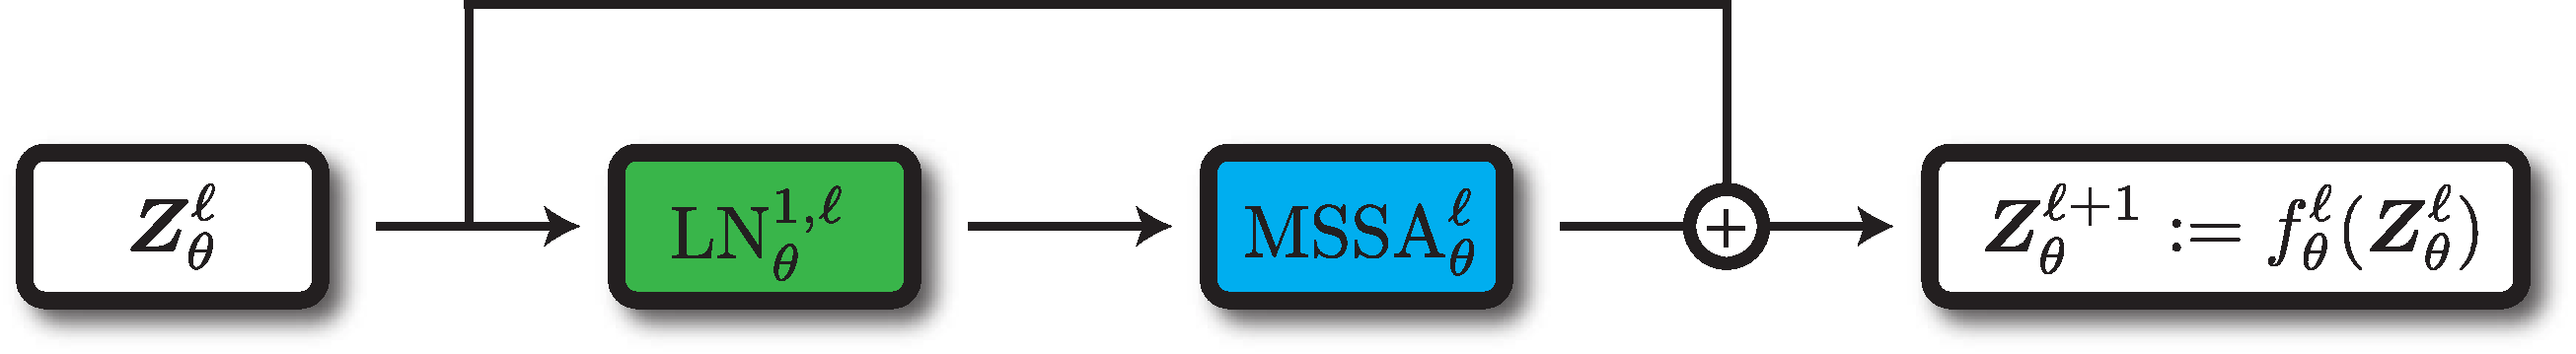
\includegraphics[width=0.7\textwidth]{\toplevelprefix/chapters/chapter7/figs/aot_backbone.pdf}
    \caption{\small\textbf{One layer of the AoT backbone.} Token representations merely go through a layer-norm and the multi-head (subspace) self-attention operator to form the layer's output. Notice that there is no token-wise nonlinearity such as MLP or ISTA or ODL.}
    \label{fig:aot_backbone}
\end{figure}


We conduct experiments using the proposed AoT architecture and demonstrate its potential. We pre-train the AoT-MSSA and AoT-MHSA models of different sizes, along with GPT-2, on OpenWebText~\citep{Gokaslan2019OpenWeb}. We plot the training loss and validation loss against the number of training iterations in \Cref{fig:loss}(a) and (b), respectively. It is observed that medium- and large-sized AoT-based models achieve training and validation losses comparable to those of the GPT-2 base model. In addition, compared to the GPT-2 base model, the AoT-MHSA model is identical to the GPT-2 base model, except for the absence of MLP layers in the architecture. As shown in \Cref{fig:loss}, incorporating MLP layers can accelerate the training process. Using the above pre-trained models, we compute the cross-entropy validation loss without training on different datasets in \Cref{tab:zeroshot}. It is observed that the AoT models with medium and large parameter sizes can achieve comparable performance to the GPT-2 base model. Moreover, we found that adding MLP layers to AoT does not improve the zero-shot performance. These results highlight the potential of attention-only models to achieve competitive results while maintaining interpretability.  

\begin{table*}[!htbp]
\caption{Zero-shot results on several language benchmark datasets and tasks: Evaluation of different sizes of AoT with the MSSA and MHSA operators and comparison to the GPT2 model.}\vskip 0.1in
\centering
\begin{small}
\begin{tabular}{l|cccccc}
\toprule
 Models  & {\bf LAMBADA} & {\bf PTB} & {\bf WikiText} & {\bf LAMBADA} & {\bf CBT CN} & {\bf CBT NE} \\
 \# of parameters  & (val loss) $\downarrow$ &  (val loss) $\downarrow$ &(val loss) $\downarrow$ & (acc) $\uparrow$ &(acc) $\uparrow$ &(acc) $\uparrow$ \\
 \midrule
 AoT-MSSA Base (102M) & 4.70 & 6.03 & 4.65 & 0.25 & 0.80 & 0.74\\
 AoT-MSSA Medium (182M) & 4.47 & 5.08 & 4.22 & 0.29 & 0.84 & 0.77 \\
 AoT-MHSA Base (122M) & 4.42 & 5.52 & 4.19 & 0.38 & 0.86 & 0.82\\
 GPT-2 Base (124M) & 4.32 & 5.75 & 4.13 &  0.40 &  0.87 &  0.84 \\
\bottomrule
\end{tabular}
\label{tab:zeroshot}
\end{small}
\end{table*} 
\vspace{-0.05in} 


\begin{figure*}[t]
\begin{center}
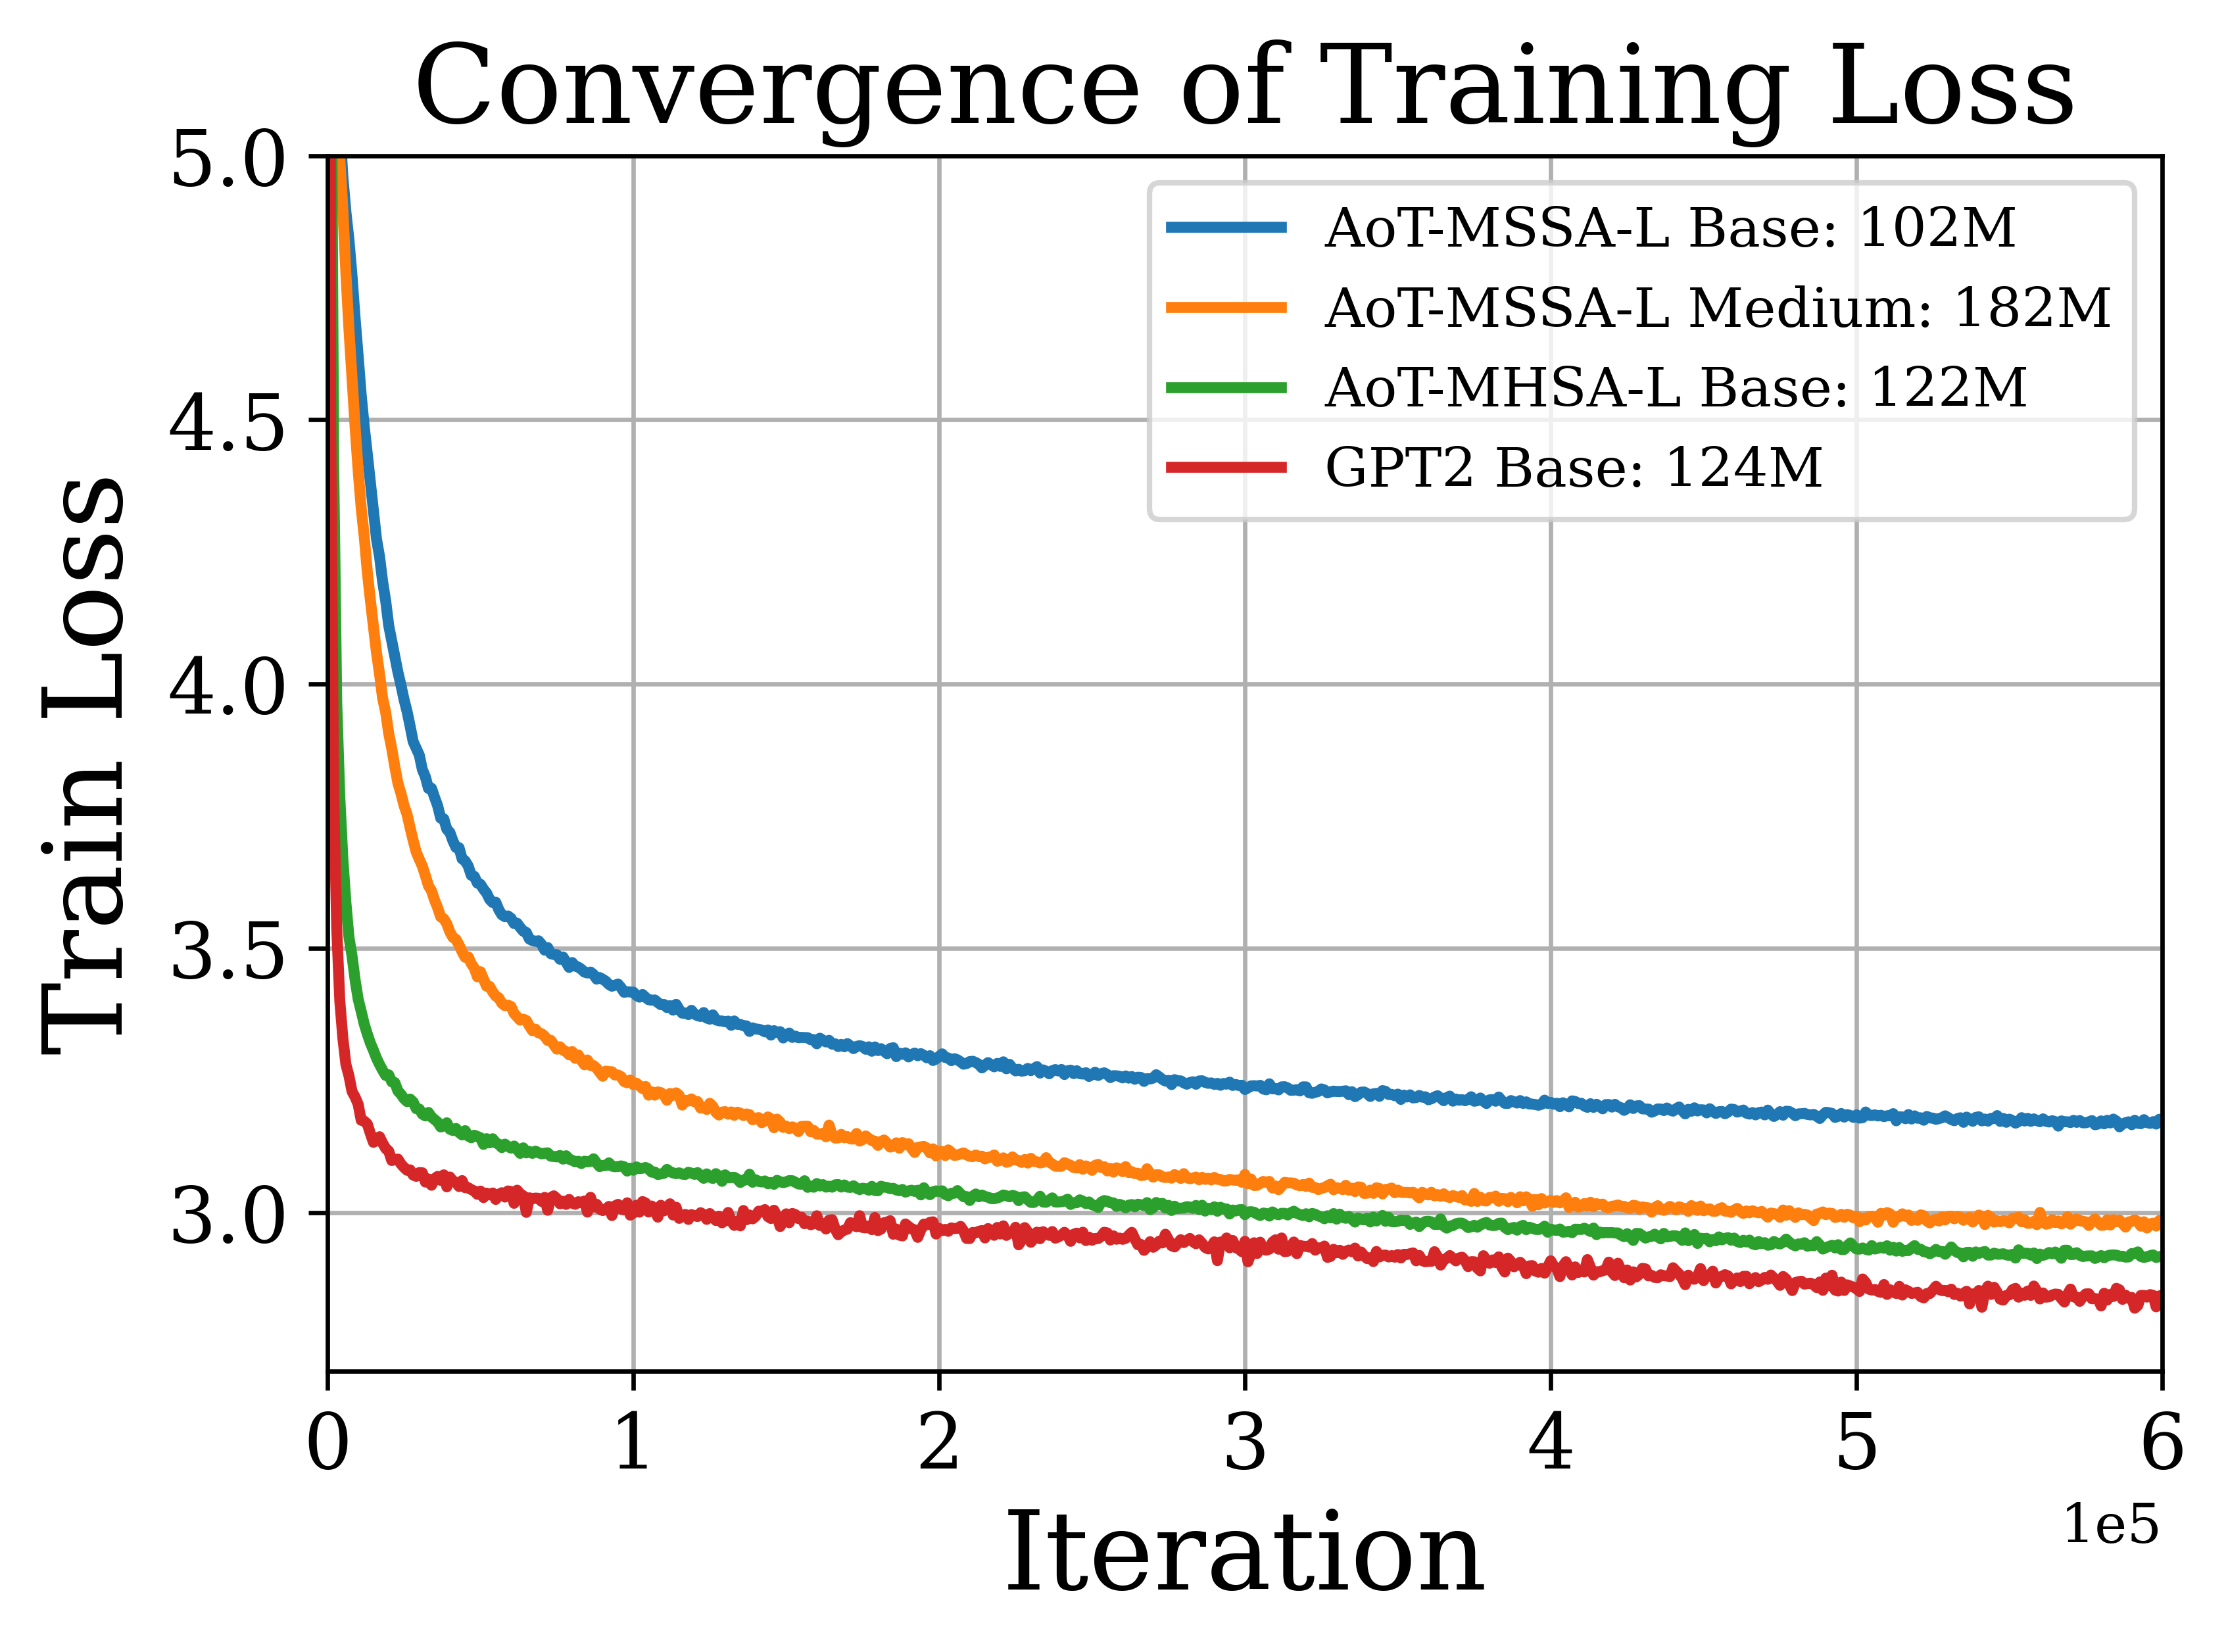
\includegraphics[width=0.4\linewidth]{\toplevelprefix/chapters/chapter7/figs/training_loss.png} \hspace{0.4in}
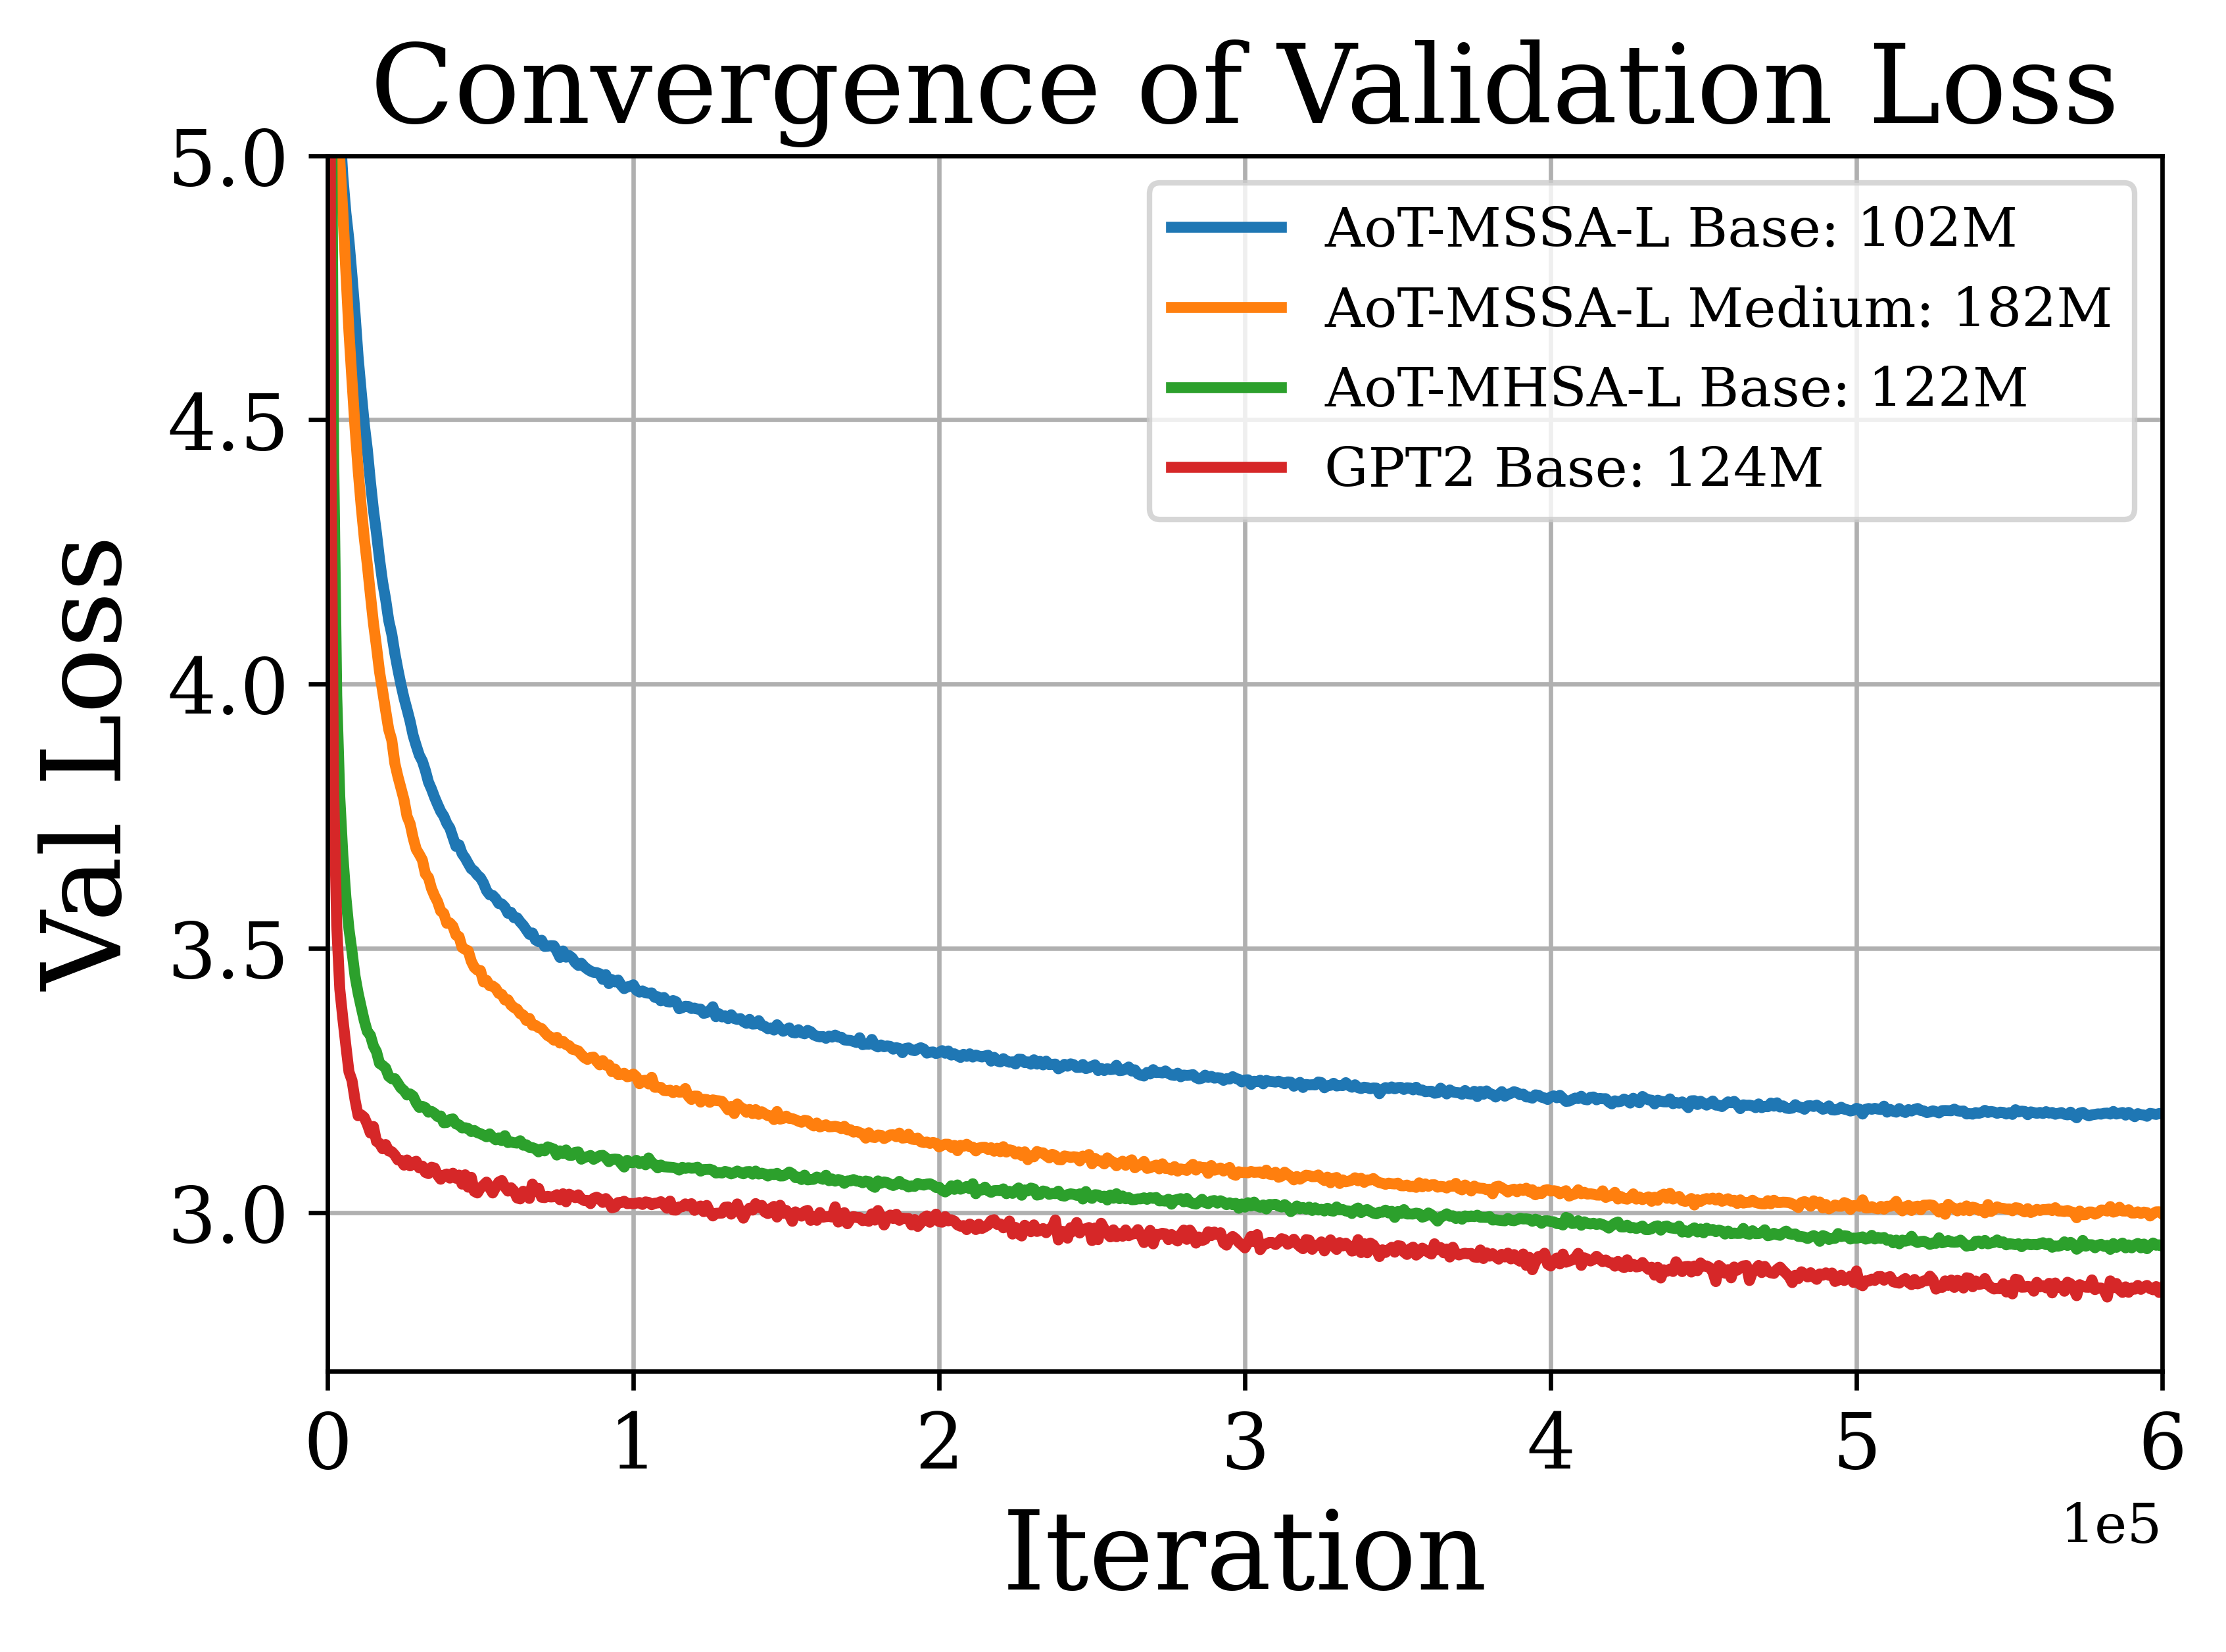
\includegraphics[width = 0.4\linewidth]{\toplevelprefix/chapters/chapter7/figs/val_loss.png}
    \vspace{-0.15in}
\caption{\centering \textbf{Evaluating models on language tasks.} We plot the training loss (left) and validation loss (right) of the AoT and GPT-2 models pretrained on OpenWebText.}  \label{fig:loss} 
\end{center}
\vspace{-0.15in}
\end{figure*} 




 

\section{Masked Autoencoding for Imagery Data}\label{sec:image_completion}

The second application we discuss is \textit{nonlinear image completion}, also known as \textit{masked autoencoding} (MAE), which is a direct generalization of the low-rank matrix completion problem discussed in \Cref{ch:classic}. Masked autoencoding, since its introduction in the deep learning context by \cite{he2022masked}, has been a staple and simple self-supervised representation learning method, which aims to endow each patch feature within \(\vZ_{\theta}\) with aggregate information as well as information about its neighbors, such that both the patch feature and aggregate features are rich sources of information for the whole sample. 

The dataset is kept the same as the image datasets discussed in \Cref{sub:contrastive_learning_data}. As usual, we still apply data augmentations to each sample in each new batch. 

\subsection{Task and Objective}\label{sub:image_completion_objective}

As the name suggests, masked autoencoding involves a view \(v_{m}\) which, given an input, performs a random resized crop (cf \Cref{sub:contrastive_learning_objective}) to turn the input image into a square image of size \((C, S_{\mask}, S_{\mask})\), then \textit{masks} (i.e., sets to zero) a fixed percentage \(p_{\mask} \in [0, 1]\) of pixels in the input. For efficiency reasons\footnote{The original implementation of MAE by \cite{he2022masked} embeds the whole image, \textit{removes} the tokens that would be masked, feeds the resulting token set through the encoder, adds back learned placeholder tokens in the masked spots and adds back the appropriate positional encoding, and feeds the resulting token set through the decoder to get the autoencoding prediction. This is more efficient since the encoder has fewer tokens to go through, but conceptually is the same as the method discussed in the text, and the resulting models' performance in the masked autoencoding task and downstream evaluations is very similar.}, the masking is done patch-wise, i.e.,  after embedding the whole image, \(p_{\mask}\) percentage of \textit{patches} are set to zero. The goal of MAE is to train an encoder \(f_{\theta} \colon \cI \to (\R^{d})^{*}\) and a decoder \(g_{\eta} \colon (\R^{d})^{*} \to \cI\) that can reconstruct an input from its masking, i.e., writing \(\hat{\vX}_{\theta, \eta} \doteq g_{\eta} \circ f_{\theta}\), we have
\begin{equation}
    \min_{\theta, \eta}\bc{\cL_{\mathrm{MAE}}(\theta, \eta) \doteq \Ex\norm{\hat{\vX}_{\theta, \eta}(\vX_{m}) - \vX}_{F}^{2}}
\end{equation}
Essentially this means that the features \(\vZ_{\theta}(\vX_{m})\) of the view \(\vX_{m} \doteq v_{m}(\vX)\) must contain information about the \textit{masked patches} as well as the existing patches. From the perspective of the compression-based white-box models in \Cref{ch:representation}, if a white-box autoencoder  \((f_{\theta}, g_{\eta})\) succeeds at this task, it means that the learned subspaces and dictionaries perform a \textit{redundant} encoding of the data such that it can reconstruct missing parts of the data from encoded other parts of the data. This means that information about each patch is stored in other patches. Therefore, each patch feature should contain both information about the patch and information about the statistics of the whole image. Thus, again, we expect that the representations should contain both local and global semantically relevant information, and therefore representations of different patches with similar local and global information should be related (i.e., on the same subspace or encoded together by a dictionary).

\subsection{Architecture}\label{sub:image_completion_architecture}

\begin{figure}
    \centering 
    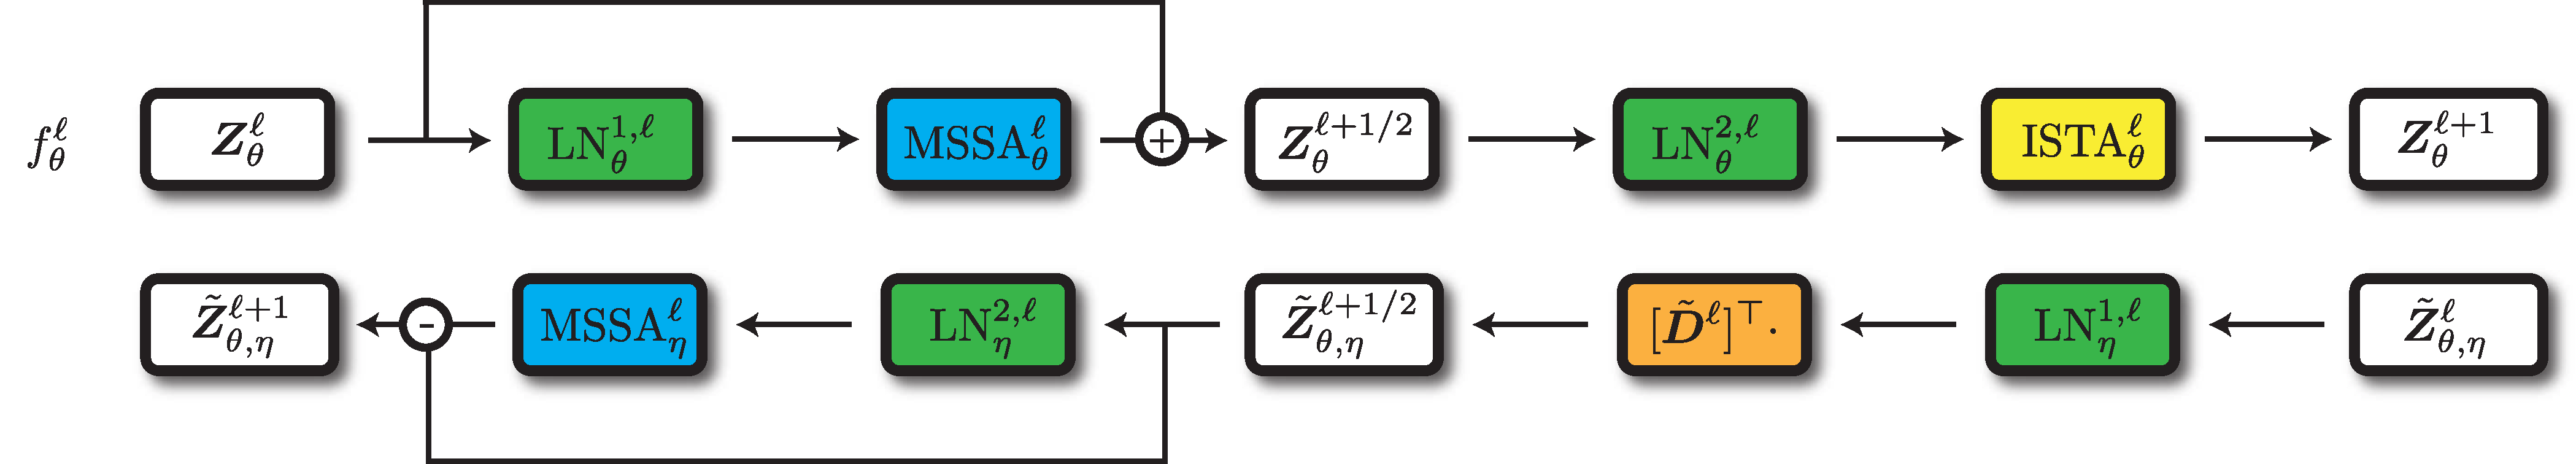
\includegraphics[width=\textwidth]{\toplevelprefix/chapters/chapter7/figs/crate_ae_backbone.pdf}
    \caption{\small\textbf{One layer of the encoder and decoder in a CRATE autoencoder backbone.} The encoder and decoder layers both feed their inputs through multi-head subspace self-attention and a dictionary learning or dictionary encoding step. Note that the encoder and decoder layers are symmetrically designed; the conceptual goal of each decoder layer is to invert an encoder layer, so this symmetry is very much by design (see e.g., \Cref{ch:autoencoding}).}
\end{figure}

We use a CRATE encoder and decoder, depicted in \Cref{fig:transformer_backbone}, though of course it is possible to use a regular transformer encoder and decoder. Details follow.

\paragraph{The encoder.} The encoder is the same as the CRATE encoder in \Cref{sub:image_classification_architecture}, with the caveat that there is no feature extractor \(f_{\theta}^{\ext}\). However, both the embedding \(f_{\theta}^{\emb}\) and the backbone \(f_{\theta}^{\backbone}\) are the same.

\paragraph{The decoder backbone.} The decoder backbone is the CRATE decoder described in \Cref{ch:autoencoding}. For completeness, we describe it now. Given a feature sequence \(\vZ_{\theta}(\vX) \doteq f_{\theta}(\vX) \in (\R^{d})^{*}\), we can process it using the decoder backbone \(g_{\eta}^{\backbone}\) as follows. The function \(g_{\eta}^{\backbone}\) is composed of \(L\) layers \(g_{\eta}^{\ell}\), i.e.,
\begin{equation}
    g_{\eta}^{\backbone} = g_{\eta}^{L} \circ \cdots \circ g_{\eta}^{1}.
\end{equation}
The layer \(g_{\eta}^{\ell}\) has the following implementation. First, define \(\tilde{\vZ}_{\theta, \eta}^{1}(\vX) \doteq \vZ_{\theta}(\vX)\). Then, we obtain
\begin{align}
    \tilde{\vZ}_{\theta, \eta}^{\ell + 1/2}(\vX) 
    &= [\tilde{\vD}^{\ell}]^{\top}\LN_{\eta}^{1, \ell}(\tilde{\vZ}_{\theta, \eta}^{\ell}(\vX)) \\ 
    \tilde{\vZ}_{\theta, \eta}^{\ell + 1}(\vX)
    &= \tilde{\vZ}_{\theta, \eta}^{\ell + 1/2}(\vX) - \MSSA_{\eta}^{\ell}(\LN_{\eta}^{2, \ell}(\tilde{\vZ}_{\theta, \eta}^{\ell + 1/2}))
\end{align}
and \(g_{\eta}^{\ell}\) is defined such that \(g_{\eta}^{\ell}(\tilde{\vZ}_{\theta, \eta}^{\ell}) \doteq \tilde{\vZ}_{\theta, \eta}^{\ell + 1}(\vX)\). Here, the relevant concept is that \(g_{\eta}^{\ell}\) should learn an approximate inverse of \(f_{\theta}^{L + 1 - \ell}\), as discretizations of a forward- and reverse-time diffusion process, respectively. In particular, \(\tilde{\vD}^{\ell}\) should approximate \(\vD^{L + 1 - \ell}\), and similarly, the \(\MSSA_{\eta}^{\ell}\) parameters should be similar to the parameters of \(\MSSA_{\theta}^{L + 1 - \ell}\). The output is \(\tilde{\vZ}_{\theta, \eta} \doteq \tilde{\vZ}_{\theta, \eta}^{L + 1}\).

\paragraph{The un-embedding module.} To transform \(\tilde{\vZ}_{\theta, \eta}(\vX)\) back into an estimate for \(\vX\), we need to undo the effect of the embedding module \(f_{\theta}^{\emb}\) using the unembedding module \(g_{\eta}^{\unemb}\). As such, harkening back to the functional form of the embedding module in \eqref{eq:definition_of_embedding_module}, i.e.,
\begin{equation}
    f_{\theta}^{\emb}(\vX) \doteq \mat{\vz_{\cls}^{1}, \vW^{\emb}f^{\patch}(\vX) + \vE^{\pos}}
\end{equation}
it implies that our inverse operation \(g_{\eta}^{\unemb}\) looks like the following:
\begin{equation}
    g_{\eta}^{\unemb}(\tilde{\vZ}) \doteq g_{\eta}^{\unemb}(\mat{\tilde{\vz}^{1}, \dots, \tilde{\vz}^{n}}) = g^{\unpatch}(\vW^{\unemb}([\tilde{\vz}^{2}, \dots, \tilde{\vz}^{n}] - \tilde{\vE}^{\pos})),
\end{equation}
where \(g^{\unpatch}\) does the inverse operation of the unrolling and flattening operation that \(f^{\patch}\) does.\footnote{Again, the ``inverse positional encoding'' \(\tilde{\vE}^{\pos}\) is learned for a large input, and for smaller inputs may be interpolated. It is even possible to directly set \(\tilde{\vE}^{\pos}\) equal to the positional encoding \(\vE^{\pos}\) and use the same interpolated positional encodings for each input in both the encoder and decoder.}

This architecture is a white-box autoencoder \((f_{\theta}, g_{\eta})\) where (recall) \(f_{\theta} = f_{\theta}^{\backbone} \circ f_{\theta}^{\emb}\) and \(g_{\eta} = g_{\eta}^{\unemb} \circ g_{\eta}^{\backbone}\). In particular, we can use it to compute an estimate for a masked view \(\hat{\vX}_{\theta, \eta}(\vX_{m}) = (g_{\eta} \circ f_{\eta})(\vX_{m})\) which should approximately equal \(\vX\) itself.

\subsection{Optimization}\label{sub:image_completion_optimization}

As in \Cref{sub:image_classification_optimization}, we use a simple optimization setup: we sample images and masks, compute the loss on those samples and the gradients of this loss, and update the parameters using a generic optimization algorithm and the aforementioned gradients. For each timestep \(k\), we:
\begin{itemize}
    \item Subsample \(B\) different samples \(\{\vX_{b}^{(k)}\}_{b = 1}^{B} \subseteq \cI\).
    \item For each sample \(\vX_{b}^{(k)}\), compute a different randomized resized crop and mask \(v_{b, m}^{(k)}\) and apply it to \(\vX_{b}^{(k)}\) to get \(\vX_{b, m}^{(k)} \doteq v_{b, m}^{t}(\X_{b}^{(k)})\).
    \item Compute the estimated autoencoding \(\hat{\vX}_{\theta, \eta}(\vX_{b, r}^{(k)}) \doteq (g_{\eta} \circ f_{\theta})(\vX_{b, r}^{(k)})\).
    \item Form the surrogate stochastic loss 
    \begin{equation}
        \hat{\cL}_{\mathrm{MAE}}^{(k)}(\theta, \eta) \doteq \frac{1}{B}\sum_{b = 1}^{B}\norm{\hat{\vX}_{\theta, \eta}(\vX_{b, r}^{(k)}) - \vX_{b}^{(k)}}_{F}^{2}.
    \end{equation}
    \item Compute one step of an optimization algorithm on \((\theta, \eta)\), giving the following iteration:
    \begin{equation}
        (\theta^{(k + 1)}, \eta^{(k + 1)}) \doteq \textsc{OptUpdate}^{(k)}(\theta^{(k)}, \eta^{(k)}; \nabla_{(\theta, \eta)}\hat{\cL}_{\mathrm{MAE}}^{(k)}).
    \end{equation}
\end{itemize}

\subsection{Evaluation} \label{sub:image_completion_optimization_1}

This is the first autoencoder network we discuss in this chapter. We use the same center crop view \(v_{\cc}\) as in \Cref{sub:contrastive_learning_evals,sub:image_classification_evals}, resizing the final image to a square with side length \(S_{\cc} = S_{\mask}\) pixels to match the shapes of the input images seen during training. 

In addition to evaluating the masked autoencoding loss itself, it is also possible to evaluate the features \(\vZ_{\theta}(\vX_{\cc})\) of the view \(\vX_{\cc} \doteq v_{\cc}(\vX)\) of the data \(\vX\) directly. For attention map fidelity evaluation, obtaining \(\vZ_{\theta}(\vX_{\cc})\) is sufficient, but for linear probing we need to extract a summarized or aggregate feature from \(\vZ_{\theta}\). To do this, we can use a (parameter-free) feature extraction map that returns the feature corresponding to the class token, i.e.,
\begin{equation}
    f_{\theta}^{\ext}(\vZ) \doteq f_{\theta}^{\ext}([\vz^{1}, \dots, \vz^{n}]) = \vz^{1},
\end{equation}
as in (for example) \Cref{sub:image_classification_objective,sub:image_classification_architecture}. With this, we have a way to obtain aggregate features \(\vz_{\theta}(\vX_{\cc}) \doteq (f_{\theta}^{\ext} \circ f_{\theta})(\vX_{\cc})\), at which point we can perform linear probing, segmentation evaluations, and so on.

\subsection{Experiments}\label{sub:image_completion_experiments}

Since CRATE-MAE is directly based on ViT-MAE, we compare the optimal settings for ViT-MAE as given by \citep{he2022masked} with the same settings applied to CRATE-MAE for a fair comparison.

\paragraph{Model architecture.} During training, the masked crop \(v_{m}\) resizes the whole image so that the shorter edge is of size \(256\) (i.e., \(S_{\rsz} = 256\)) before taking a random crop of size \(224 \times 224\) (i.e., \(S_{\mathrm{mask}} = 224\)), and masking \(p_{\mathrm{mask}} = \frac{3}{4}\) of the patches. We take patch size \(16\) (i.e., \(P_{H} = P_{W} = 16\)). We use the small and base variants of the ViT-MAE architecture as the embedding and backbone for both the encoder and decoder, swapping out the MHSA and MLP components for MSSA, ISTA, and linear layers, respectively. We use the same number of heads and head dimension in the case of MSSA. However, the original ViT-MAE uses an encoder which uses nearly all the total layers and a decoder which only uses a few layers; we allocate half the total number of layers (which stays the same from ViT-MAE to CRATE-MAE) to our encoder and decoder, as suggested by the conceptual and theoretical framework in \Cref{ch:autoencoding}. For CRATE-MAE we set \((\beta, \lambda) = (1, 0.1)\).

\paragraph{Datasets and optimization.} For pre-training, we use the ImageNet-1K dataset. We use the AdamW optimizer to pre-train both our ViT-MAE replication as well as CRATE-MAE. We set the base learning rate as \(3 \times 10^{-5}\), the weight decay as \(0.1\), and batch size as \(B = 4096\). Our learning rate schedule increases the learning rate linearly to the base learning rate over the first \(40\) epochs, and decreases to \(0\) using a cosine schedule over the next \(760\) epochs (training all models for \(800\) epochs each). For pre-training, we apply the usual regime of data augmentations (flips, Gaussian blurs, solarization, etc) to the image data.

For linear probing, we use several evaluation datasets such as CIFAR10, CIFAR100, Oxford-Flowers, and Oxford-IIT-Pets. For linear probing, we precompute the features of all samples in the target dataset and apply a fast linear regression solver, e.g., from a standard package such as Scikit-Learn.

\paragraph{Experiment results.} \Cref{tab:crate_mae_linear_probing} demonstrates that CRATE-MAE models achieve, roughly speaking, parity with the popular ViT-MAE architecture at similar parameter counts, and also that the feature learning performance (as measured by performance on downstream classification tasks) increases with scale. Meanwhile, \Cref{fig:crate_mae_semantic_heads} demonstrates that the encoder saliency maps (and therefore the fine-grained features learned by the encoder) indeed isolate and highlight the key parts of the input image.


\begin{table}
    \centering 
    \begin{tabular}{@{}lcc|cc@{}}
        \toprule 
        \textbf{Model} & CRATE-MAE-S(mall) & CRATE-MAE-B(ase) & {\color{gray} ViT-MAE-S} & {\color{gray} ViT-MAE-B} \\
        \midrule
        \midrule
        \# parameters & 25.4M & 44.6M & 47.6M & {\color{gray}143.8M} \\
        \midrule
        CIFAR10 & 79.4 & 80.9 & {\color{gray} 79.9} & {\color{gray} 87.9} \\
        CIFAR100 & 56.6 & 60.1 & {\color{gray} 62.3} & {\color{gray} 68.0} \\
        Oxford Flowers-102 & 57.7 & 61.8 & {\color{gray} 66.8} & {\color{gray} 66.4} \\
        Oxford-IIIT-Pets & 40.6 & 46.2 & {\color{gray} 51.8} & {\color{gray} 80.1} \\
        \bottomrule
    \end{tabular}
    \caption{\small\textbf{Linear probing classification accuracy of CRATE-MAE and ViT-MAE} on various datasets with different model sizes when the backbone is pre-trained for masked autoencoding on ImageNet-1K. Given the same parameter count, CRATE-MAE achieves roughly similar performance while simultaneously enjoying a simpler and more principled architecture design.}
    \label{tab:crate_mae_linear_probing}
\end{table}

\begin{figure}
    \centering 
    \includegraphics[width=\textwidth]{\toplevelprefix/chapters/chapter7/figs/crate_mae_semantic_heads.pdf}
    \caption{\small\textbf{Saliency maps of CRATE-MAE.} Each pair of images consists of the original image (left) and a selected saliency map (right) corresponding to an attention head in the last layer. As is usual for CRATE models, but unusual for general transformer-like models, the saliency maps correspond to the objects in the input image.}
    \label{fig:crate_mae_semantic_heads}
\end{figure}





\section{Summary and Notes}

All work in this chapter is downstream of the Transformer architecture, which was introduced by \citet{vaswani2017attention}. The Transformer architecture is formally described in \Cref{sec:contrastive_learning}. A main empirical innovation in recent years, spurred by the prevalence and performance of the Transformer architecture, is to formulate a given learning problem as a sequence-to-sequence problem and apply the Transformer architecture. This has enabled the Transformer architecture to be essentially ubiquitous in (almost) all deep learning applications. As such, direct improvements to the Transformer can propagate to become solutions to many problems and have considerable impact; similarly, we can apply our white-box understanding of transformer-like architectures to many modern problems. The material covered in this chapter is merely a subset of the work that has already been done; other work includes masked completion for text data (i.e., BERT) \citep{devlin2019bert,yu2024white}, (mechanistic) interpretability of language and vision models \citep{bai2024improving}, and error correcting coding \citep{zheng2025white}. There is much more to do.

There is also much more theory specifically about the practice of scaling neural networks, which is enormously practically viable, and we at least remark on it here. This line of work was popularized by the ``Tensor Programs'' line of work \citep{yang2022tensor}. The basic prescription is that we want the initial gradient updates in a transformer to be constant size, and by working through the backpropagation equations (\Cref{app:optimization}) carefully, we can determine the scale of the initialization and learning rates (chosen layer-wise) that are required to achieve this. In practice, such prescriptions greatly increase the stability and convergence of training at large scales; they also prescribe a way to find the ``optimal''\footnote{The word ``optimal'' is used in quotes because the work on this merely uses some desiderata about the weight size, feature size, and gradient size at initialization to determine ``optimality'', as opposed to, say, the test loss at convergence.} hyperparameters for large-scale training using only small-scale training. Follow-ups to this work attempt to accommodate the feature geometry \citep{bernstein2024oldoptimizernewnorm}, which could be informed by the work in this book about representation learning. Other follow-ups incorporate this weight-wise information into the optimizer itself to obtain these scaling benefits automatically, obtaining optimizers such as Muon \citep{jordan6muon}, which have recently been used for training trillion-parameter models very stably \citep{moonshot2025kimi}. Overall, the two approaches to deep learning theory are orthogonal or complementary.


\section{Exercises and Extensions}

\begin{exercise}
    Read the DINO paper \cite{caron2021emerging}.
\end{exercise}

\begin{exercise}
    DINO v2 \cite{oquab2023dinov2} uses everything from DINO v1 but also, during the data augmentation phase, randomly masks out patches within each view. This kind of augmentation should enforce that the features of images with similar local information are similar. Formulate an optimization problem that promotes this in the encoder, and implement it.
\end{exercise}


\begin{exercise}
    This exercise considers the implementation of stochastic optimization algorithms to minimize losses involving expectations.
    \begin{enumerate}[(a)]
        \item Propose an alternative to the term involving \(R_{\eps}\) in \eqref{eq:simdino_loss_teacherstudent_empirical} for approximating the covariance regularization term in \eqref{eq:simdino_loss_teacherstudent}. Evaluate the time complexity required to compute your proposed term and its gradient. Include an analysis for computing it on a single compute node vs.~multiple nodes.
        \item Evaluate the time complexity required to compute the existing term in \eqref{eq:simdino_loss_teacherstudent_empirical} and its gradient.
    \end{enumerate}
\end{exercise}

\begin{exercise}
    Prove that \eqref{eq:linear_probing} and \eqref{eq:linear_probing_empirical} are convex optimization problems.
\end{exercise}

\begin{exercise}
    \phantom{}
    \begin{enumerate}[(a)]
        \item Implement the CRATE and CRATE-\(\alpha\) models.
        \item Compare their performance and efficiency on the CIFAR-10 dataset.
        \item Compare their interpretability in two ways:
        \begin{itemize}
            \item The sparsity \(\norm{\vZ}_{0}\) of the representation \(\vZ\)
            \item The attention maps \(\va_{\theta}^{k, \ell}\)
        \end{itemize}
    \end{enumerate}
\end{exercise}

\end{document}
